\documentclass[a4paper,12pt,oneside]{ThesisStyle}

\usepackage[toc,page]{appendix}

\newcommand{\nocontentsline}[3]{}
\newcommand{\tocless}[2]{\bgroup\let\addcontentsline=\nocontentsline#1{#2}\egroup}

%\usepackage[style=verbose]{biblatex}

\usepackage{listings}
\usepackage{color}
\usepackage[utf8]{vietnam}
%\usepackage[monochrome]{color} %enable to make black-while print version
\usepackage{arial}	% same Time New Roma
\usepackage{titlesec}
\usepackage{subcaption}
\usepackage{amsmath}
\titleformat
{\chapter} % command
[display] % shape
{\bfseries\LARGE} % format
{\Large{Chapter} \ \thechapter} % label
{0.5ex} % sep
{
    \rule{\textwidth}{1pt}
    \vspace{1ex}
    \centering
} % before-code
[
\vspace{-0.5ex}%
\rule{\textwidth}{0.3pt}
] % after-code


\titlespacing*{\chapter}{0pt}{-1cm}{1cm}


%\end trong add

\usepackage{tabularx}
\usepackage{multirow}
\usepackage{pdf14}
\usepackage{pgfplots}
\usetikzlibrary{calc}
\usepackage{booktabs}
\usepackage{array}
\usepackage{tikz}
\usepackage{amsmath,amssymb}             % AMS Math
\usepackage[left=3cm,right=2cm,top=2cm,bottom=2cm,includefoot,includehead,headheight=13.6pt]{geometry}

\usepackage{floatrow}
\floatsetup[table]{capposition=top}
\usepackage{multirow}
\usepackage[english]{babel}
\usepackage[format=plain,indention=1em]{caption}
\usepackage{float}
\usepackage{booktabs}
\newcommand\abs[1]{\left|#1\right|}

\renewcommand{\baselinestretch}{1.05}

% Table of contents for each chapter

\usepackage[nottoc, notlof, notlot]{tocbibind}
\usepackage{minitoc}
\setcounter{minitocdepth}{2}
\mtcindent=15pt
% Use \minitoc where to put a table of contents

\usepackage{aecompl}

% Glossary / list of abbreviations

\usepackage[intoc]{nomencl}
\renewcommand{\nomname}{List of Abbreviations}

\makenomenclature

% My pdf code

\usepackage{ifpdf}

\ifpdf
  %\usepackage[pdftex]{graphicx}
  \DeclareGraphicsExtensions{.jpg}
  \usepackage[a4paper,pagebackref,hyperindex=true]{hyperref}
\else
  \usepackage{graphicx}
  \DeclareGraphicsExtensions{.ps,.eps}
  \usepackage[a4paper,dvipdfm,pagebackref,hyperindex=true]{hyperref}
\fi

\graphicspath{{.}{images/}}

% nicer backref links
\renewcommand*{\backref}[1]{}
\renewcommand*{\backrefalt}[4]{%
\ifcase #1 %
(Not cited.)%
\or
(Cited on page~#2.)%
\else
(Cited on pages~#2.)%
\fi}
\renewcommand*{\backrefsep}{, }
\renewcommand*{\backreftwosep}{ and~}
\renewcommand*{\backreflastsep}{ and~}

% Links in pdf
\usepackage{color}
\definecolor{linkcol}{rgb}{0,0,0.4} 
\definecolor{citecol}{rgb}{0.5,0,0} 
\definecolor{gray}{rgb}{0.4,0.4,0.4}
\definecolor{darkblue}{rgb}{0.0,0.0,0.6}
\definecolor{cyan}{rgb}{0.0,0.6,0.6}

\lstset{
  basicstyle=\ttfamily,
  columns=fullflexible,
  showstringspaces=false,
  commentstyle=\color{gray}\upshape
}

\lstdefinelanguage{XML}
{
  morestring=[b]",
  morestring=[s]{>}{<},
  morecomment=[s]{<?}{?>},
  stringstyle=\color{black},
  identifierstyle=\color{darkblue},
  keywordstyle=\color{cyan},
  morekeywords={annotation, folder, filename, path, source, size, width, height, depth, segmented, object, name, pose, truncated, difficult, bndbox, xmin, ymin, xmax, ymax, database}% list your attributes here
}

% Change this to change the informations included in the pdf file

% See hyperref documentation for information on those parameters

\hypersetup
{
bookmarksopen=true,
pdftitle="Design and Use of Anatomical Atlases for Radiotherapy",
pdfauthor="Olivier COMMOWICK", 
pdfsubject="Creation of atlases and atlas based segmentation", %subject of the document
%pdftoolbar=false, % toolbar hidden
pdfmenubar=true, %menubar shown
pdfhighlight=/O, %effect of clicking on a link
colorlinks=true, %couleurs sur les liens hypertextes
pdfpagemode=None, %aucun mode de page
pdfpagelayout=SinglePage, %ouverture en simple page
pdffitwindow=true, %pages ouvertes entierement dans toute la fenetre
linkcolor=linkcol, %couleur des liens hypertextes internes
citecolor=citecol, %couleur des liens pour les citations
urlcolor=linkcol %couleur des liens pour les url
}

% definitions.
% -------------------

\setcounter{secnumdepth}{3}
\setcounter{tocdepth}{2}

% Some useful commands and shortcut for maths:  partial derivative and stuff

\newcommand{\pd}[2]{\frac{\partial #1}{\partial #2}}
%\def\abs{\operatorname{abs}}
\def\argmax{\operatornamewithlimits{arg\,max}}
\def\argmin{\operatornamewithlimits{arg\,min}}
\def\diag{\operatorname{Diag}}
\newcommand{\eqRef}[1]{(\ref{#1})}

\usepackage{rotating}                    % Sideways of figures & tables
%\usepackage{bibunits}
%\usepackage[sectionbib]{chapterbib}          % Cross-reference package (Natural BiB)
%\usepackage{natbib}                  % Put References at the end of each chapter
                                         % Do not put 'sectionbib' option here.
                                         % Sectionbib option in 'natbib' will do.
\usepackage{fancyhdr}                    % Fancy Header and Footer

% \usepackage{txfonts}                     % Public Times New Roman text & math font
  
%%% Fancy Header %%%%%%%%%%%%%%%%%%%%%%%%%%%%%%%%%%%%%%%%%%%%%%%%%%%%%%%%%%%%%%%%%%
% Fancy Header Style Options

\pagestyle{fancy}                       % Sets fancy header and footer
\fancyfoot{}                            % Delete current footer settings

%\renewcommand{\chaptermark}[1]{         % Lower Case Chapter marker style
%  \markboth{\chaptername\ \thechapter.\ #1}}{}} %

%\renewcommand{\sectionmark}[1]{         % Lower case Section marker style
%  \markright{\thesection.\ #1}}         %

\fancyhead[LE,RO]{\bfseries\thepage}    % Page number (boldface) in left on even
% pages and right on odd pages
\fancyhead[RE]{\bfseries\nouppercase{\leftmark}}      % Chapter in the right on even pages
\fancyhead[LO]{\bfseries\nouppercase{\rightmark}}     % Section in the left on odd pages

\let\headruleORIG\headrule
\renewcommand{\headrule}{\color{black} \headruleORIG}
\renewcommand{\headrulewidth}{1.0pt}
\usepackage{colortbl}
\arrayrulecolor{black}

\fancypagestyle{plain}{
  \fancyhead{}
  \fancyfoot{}
  \renewcommand{\headrulewidth}{0pt}
}

\usepackage{algorithm}
\usepackage[noend]{algorithmic}
\usepackage[algo2e,ruled,lined,boxed,linesnumbered]{algorithm2e}

%%% Clear Header %%%%%%%%%%%%%%%%%%%%%%%%%%%%%%%%%%%%%%%%%%%%%%%%%%%%%%%%%%%%%%%%%%
% Clear Header Style on the Last Empty Odd pages
\makeatletter

\def\cleardoublepage{\clearpage\if@twoside \ifodd\c@page\else%
  \hbox{}%
  \thispagestyle{empty}%              % Empty header styles
  \newpage%
  \if@twocolumn\hbox{}\newpage\fi\fi\fi}

\makeatother
 
%%%%%%%%%%%%%%%%%%%%%%%%%%%%%%%%%%%%%%%%%%%%%%%%%%%%%%%%%%%%%%%%%%%%%%%%%%%%%%% 
% Prints your review date and 'Draft Version' (From Josullvn, CS, CMU)
\newcommand{\reviewtimetoday}[2]{\special{!userdict begin
    /bop-hook{gsave 20 710 translate 45 rotate 0.8 setgray
      /Times-Roman findfont 12 scalefont setfont 0 0   moveto (#1) show
      0 -12 moveto (#2) show grestore}def end}}
% You can turn on or off this option.
% \reviewtimetoday{\today}{Draft Version}
%%%%%%%%%%%%%%%%%%%%%%%%%%%%%%%%%%%%%%%%%%%%%%%%%%%%%%%%%%%%%%%%%%%%%%%%%%%%%%% 

\newenvironment{maxime}[1]
{
\vspace*{0cm}
\hfill
\begin{minipage}{0.5\textwidth}%
%\rule[0.5ex]{\textwidth}{0.1mm}\\%
\hrulefill $\:$ {\bf #1}\\
%\vspace*{-0.25cm}
\it 
}%
{%

\hrulefill
\vspace*{0.5cm}%
\end{minipage}
}

\let\minitocORIG\minitoc
\renewcommand{\minitoc}{\minitocORIG \vspace{1.5em}}

\usepackage{multirow}
\usepackage{slashbox}

\newenvironment{bulletList}%
{ \begin{list}%
	{$\bullet$}%
	{\setlength{\labelwidth}{25pt}%
	 \setlength{\leftmargin}{30pt}%
	 \setlength{\itemsep}{\parsep}}}%
{ \end{list} }

\newtheorem{definition}{Définition}
\renewcommand{\epsilon}{\varepsilon}

% centered page environment

\newenvironment{vcenterpage}
{\newpage\vspace*{\fill}\thispagestyle{empty}\renewcommand{\headrulewidth}{0pt}}
{\vspace*{\fill}}

\newcommand*{\tabbox}[2][t]{%
    \vspace{0pt}\parbox[#1][3.7\baselineskip]{3cm}{\strut#2\strut}}
\newtheorem{theorem}{Theorem}

\begin{document}

\begin{titlepage}
\thispagestyle{empty}
%Border
\begin{tikzpicture}[remember picture, overlay]
  \draw[line width = 3pt] ($(current page.north west) + (2cm,-1.5cm)$) rectangle ($(current page.south east) + (-1cm,1.5cm)$);
\end{tikzpicture}
\begin{tikzpicture}[remember picture, overlay]
  \draw[line width = 1pt] ($(current page.north west) + (1.9cm,-1.4cm)$) rectangle ($(current page.south east) + (-0.9cm,1.4cm)$);
\end{tikzpicture}
\vspace{-2cm}
\begin{center}
\large 
	\bfseries{HO CHI MINH UNIVERSITY OF TECHNOLOGY} \\ [0.3cm]
	\bfseries{COMPUTER SCIENCE AND COMPUTER ENGINEERING DEPARTMENT} \\
\end{center}

\vspace{0.4cm}
\begin{center}

\includegraphics[scale=0.35]{hcmut.png}\\[1cm]
\end{center}
\vspace{-0.75cm}
\begin{center}
\large 
	\bfseries BACHELOR DISSERTATION \\
\end{center}
%\rule{\textwidth}{1pt}
\vspace{-1.25cm}
\begin{center}
\Large
	\begin{tabular}{@{}c}
	 	\bfseries{A SYSTEM TO COLLECT AND ANALYZE IMAGE}\\  
		\bfseries{AND VIDEO DATA USING CROWDSOURCING} \\     
		\bfseries{MODEL AND DEEP LEARNING TECHNIQUES} \\ 
		\bfseries{ FOR SOCIAL SECURITY} \\[0.5cm] 

	\end{tabular}
\end{center}
%\rule{\textwidth}{1pt}\\[1cm]
	
\hspace{4.5cm}	
\begin{minipage}[t]{0.7\linewidth}
\large
	\textbf{HỘI ĐỒNG: HỆ THỐNG THÔNG TIN}\\ [0.5cm]
	\textbf{GVHD: PSG. TS. Đặng Trần khánh}\\ [0.5cm]
	\textbf{GVPB: TS. ...}\\
	\vspace{-0.7cm}
	\begin{center}
	\textbf{---o0o---}
	\end{center}
	\textbf{SVTH 1: Đinh Duy Kha ()}\\ [0.5cm]
	\textbf{SVTH 2: Võ Tuấn Kiệt (1450241)}\\[0.5cm]
	\textbf{SVTH 3: Phạm Hồng Thái ()}\\[0.5cm]
	\textbf{SVTH 4: Vũ Minh Trí ()}\\[0.5cm]
	\textbf{SVTH 5: Nguyễn Khánh Nam ()}\\[0.5cm]
\end{minipage}

\vfill
\centerline{\large{TP. HỒ CHÍ MINH, THÁNG 06 NĂM 2018}}
\end{titlepage}

\dominitoc

\pagenumbering{roman}

\cleardoublepage

\chapter*{COMMITMENT}
We guarantee the bachelor thesis \textit{A System to collect and analyze image/video data using crowd-sourcing model and deep learning techniques for social security} is a scientific research conducted by ourselves under supervision of \textbf{Assoc. Prof, PhD Đặng Trần Khánh}. Results are obtained through progress of learning and analyzing objectively based on practice of the project. 
\\
Statistics and number originated from other research are mentioned following scientific principle. Results in this report haven't been published in any report.

\begin{flushright}
Ho Chi Minh City, December 24th 2018
\end{flushright}
\hspace{11cm} Thesis authors \\
\vspace{3cm}

\cleardoublepage

\chapter*{ACKNOWLEDGEMENTS}
Firstly, we would like to express my sincere gratitude to my advisor \textbf{Assoc. Prof, PhD Dang Tran Khanh} for the continuous support of our thesis, for his patience, motivation, and immense knowledge. His guidance helped us in all the time of research and writing of this thesis. We could not have imagined having a better advisor and mentor for our research.
\\
\\
Besides my advisor, we would like to thank all of our lecturers, mentors, who has been dedicated to instruct us in our study since we attended at our university
\\
\\
Finally, we must express our profound gratitude to authors of published research used in our thesis. This accomplishment would not have been possible without them.

\begin{flushright}
Ho Chi Minh City, December 24th 2018 \\
\hfill \\
Vũ Minh Trí, Võ Tuấn Kiệt, Phạm Hồng Thái, Đinh Duy Kha, Nguyễn Khánh Nam
\end{flushright}

\cleardoublepage

\chapter*{SUMMARY}


\cleardoublepage

%%%%%%%%%%%%%%%%%%% mục lục %%%%%%%%%%%%%%%%%%%
% \renewcommand{\contentsname}{MỤC LỤC}
% \renewcommand{\listfigurename}{MỤC LỤC HÌNH}
% \renewcommand{\listtablename}{MỤC LỤC BẢNG}
% \renewcommand{\figurename}{Hình}
% \renewcommand{\tablename}{Bảng}

\newcommand{\footcaption}[1]{\caption[#1]{#1\footnotemark.}}

\tableofcontents
\listoffigures 
\listoftables

\cleardoublepage

\chapter*{Glossary of Terms }

{\renewcommand{\arraystretch}{1.5}
\begin{table}[H]
    \begin{tabular}{p{4cm}  p{9cm}}    
     DNN & Deep learning Neural Network \\
     ANN & Artificial Neural Network \\
     CNN & Convolutional Neural Network \\
     R-CNN & Regional Convolutional Neural Network \\
     RoI & Region of Interest \\
     ML  & Machine Learning\\
     DL & Deep Learning \\	
     SVM & Support Vector Machine\\     
     RoI & Region of Interest \\
     RPN & Region Proposal Network \\
     BBox & Bounding Box \\
     GD & Gradient Descent\\
     NMS & Non-Max Suppression \\
	\end{tabular}   
\end{table}


\mainmatter

\chapter{INTRODUCTION}
\label{introduction}
\section{Motivation}
Along with the development of technology, data is generated with a tremendous volume. According to the statistic, Facebook users upload 250 billion photos, and 350 million new images each day \footnote{Source: \url{https://www.businessinsider.com/facebook-350-million-photos-each-day-2013-9}}. In 2016, 47 \% of Vietnamese population have access to the Internet (World bank). This explosion of data enable the opportunity to analyze and extract valuable information.

One of the things that support the advancement of Deep Learning is the massive amount of data that is available today. This enables Neural Networks to really show their potential since they get better the more data you fed into them. Neural network is one of the most effective technique to derive information from data. In recent years, advancements in Neural Networks significantly enhanced the development of computer vision field. On the famous ImageNet \footnotetext{Source: \url:{http://www.image-net.org/challenges/LSVRC/}}dataset, trained neural networks can now generate results that are better than human in classifying images (Figure \ref{chap3:deeplearning_vs_human}). 

\begin{center}
    \begin{figure}[H]
    \centering
    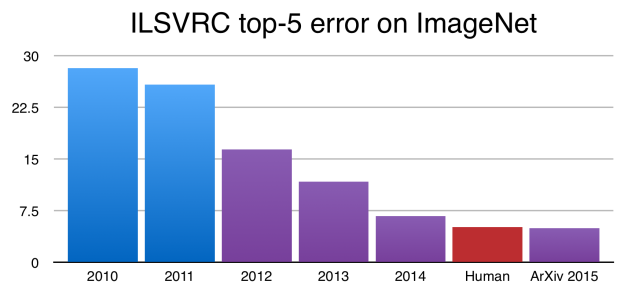
\includegraphics[width=0.75\columnwidth]{images/chap3/deeplearning_vs_human.png}
    \footcaption{Neural Network out-performing human in 2015 on ImageNet Large Scale Visual Recognition Challenge}
    \label{chap3:deeplearning_vs_human}
    \end{figure}
\end{center}
\footnotetext{Source: \url:{ https://devblogs.nvidia.com/mocha-jl-deep-learning-julia/}}
Availability of data and advancement of deep-learning poses a solution to strengthen the security: Collecting data and using deep learning to analyze collected data to improve security. 
In this modern and fast paced world, security is more important than ever. It is one of the fastest growing industries in the world today.
Almost everyday one hears about damage or loss occurring due to security lapses or a lack of security on the news. 

\section{Thesis statement}
\subsection{Goal}
The goal of this thesis is to build a system to collect and analyze image/video data using crowd-sourcing model and deep learning techniques for social security. The system require these features:
\begin{itemize}
	\item Using crowd-sourcing technique to collect image/video from users.
	\item Collected data are saved into a database.
	\item Extract valuable information from collected data using deep learning.
	\item Extracted information is also saved to database and used for security matter
\end{itemize} 
The main task of the project are:
\begin{itemize}
	\item Create an user interface to interact with users. The interface allows users to upload image/video and provide as much as information about the data to the system.
	\item Design a database which is able to save data, information about data, extracted information from data,...
	\item Design a deep learning model to extract information from data.
	\item Using extracted information to notify users about security problem.
\end{itemize} 
\subsection{Challenges}
This thesis is able to identify some challenges to the goal of this thesis:
\begin{itemize}
	\item Developing a video analyzing system requires a large amount of data. However, there are no video dataset of the environment of Vietnam.
	\item There are currently no system in Vietnam that does the job of crowd-sourcing data, so a system has to be developed for this specific task.
	\item 
\end{itemize}
\subsection{Stages}
With specified tasks, the thesis is divided into 6 main stages:
\begin{itemize}
	\item Stage 1: Study and research crowd-sourcing methods, background theory of machine learning in general and deep learning in particular. Especially, research deep learning models appropriate to extract information from image/video
	\item Stage 2: Implement a module to handle image. 
	\item Stage 3: Design an applicable database.
	\item Stage 4: Implement a interface to interact with user.
	\item Stage 5: Implement a module to handle video
	\item Stage 6: Complete the system by connecting interface, image handling module, video handling module together. Output from image/video handling module is used to notify user about security problem through the interface.
\end{itemize} 
In the proposal of this thesis, stage 1 and 2 of the project are done, the remaining stages are finished in this thesis.
  
\section{Scientific and Practical contributions}
\subsection{Scientific contributions}
Develop a system to collect data and allow user to interact with it through posting and notifications. \\
By applying Deep Learning and Computer Vision theories and by utilizing the Keras framework with a Tensorflow backend, some video classification techniques can be re-implemented and benchmarked. Subsequently, the team is able to apply those techniques to a real-world problem which is finding suspicious activities in videos \\ %FIX.
In addition, those classifying models are deployed with performance in mind using NGINX, Gunicorn and Flask framework.
\subsection{Practical contributions}
The thesis proposes a system to improve security of neighborhoods. Such system can be beneficial to the residents as it assure their safety.
\section{Thesis scope}
Currently, building a system to enhance security for a whole city is impractical due to limited resources. The thesis focuses on building the system to raise security within a scope of a neighborhood. The scope can be freely expanded with additional resources in the future.
\section{Report overview}
\begin{itemize}
	\item Chapter 1: Introduce the main goal of the thesis, planned stages to conduct the project, overview of the report.
	\item Chapter 2: Background knowledge about crowd-sourcing, ANN, CNN, RNN.
	\item Chapter 3: Propose a solution for crowd-sourcing model: a social media website; Extracting information from image: face recognition; Extracting information from video: video classification.
	\item Chapter 4: The implementation of the social media website, face recognition module, video classifier module and connection between them.
	\item Chapter 5: Evaluation of the social media website.
	\item Chapter 6: Result, limitation and how to resolve these challenges, further development in the future.
\end{itemize} 


\cleardoublepage

\chapter{BACKGROUND KNOWLEDGE}
\label{chap:background}

\paragraph{Chapter 2} Presentation of background knowledge necessary for the implementation process, including the content: crowd-sourcing, ANN, CNN, RNN.

\section{Crowd-sourcing}
\subsection{Definition}
Crowdsourcing is a relatively new approach for knowledge acquisition, information diffusion, the exchange of thoughts and views among experts and the crowd, etc \cite{futureinternet0600109}. Based on this approach, several kinds of problems can be distributed and resolved through the adoption of appropriate web-based platforms designed for such a purpose. The exploitation of collective knowledge and intelligence results in the creation of innovative ideas, where in some cases, participants earn money or gain a “prize” as acknowledgment for their contribution. The advent of the World Wide Web and the spread of the Internet have led to the development of online systems through which people from all over the world have the opportunity to participate in a problem solving process with or without the contribution of experts. 

Therefore, crowdsourcing can be considered as a process evolving through the following steps: the online release of a problem, the generation of alternative solutions by the crowd (participants), the evaluation of the proposed solutions, the selection of the best provided solution and the exploitation of the selected solution by the company or institution that initially posted the problem online.

 Among the most representative crowdsourcing applications that have been developed with the upport of the so-called “crowdsourced” information are Wikipedia, Waze (a free turn-by-turn GPS application for mobile phones that uses crowd-ourcing to provide routing and real-time traffic updates), Arcbazar (an American crowd-surcing platform for architectural design services), Facebook (used crowd-sorcing to create different language versions of its site) and OSM (OpenStreetMap).
 
  As mentioned above, crowdsourcing is based on the principle that nobody knows everything, as everyone has a share in knowledge. In this context, the “wisdom of the crowd” can be utilized during the problem solving process through the “aggregation” of several proposed solutions \cite{doi101177}. Such a process can be facilitated by the adoption of new web technologies that offer the crucial advantage of “bringing people together”. Different views and perspectives can lead to different solutions, some of which may be unexpectedly remarkable.
  
  
  On the other hand, participants in a crowdsourcing process gain several benefits. They acquire new skills. They perceive the “seeking to the best solution” process as a challenge to achieve, and they also gain new knowledge. In some cases, they can also “incorporate that experience in the seeking of better employment or in the goal of establishing oneself in freelance work as an entrepreneur” \cite{doi101177}. Crowdsourcing is a model appropriate for the utilization of collective talents by aggregating collective intelligence and knowledge and also by increasing the ingenuity of the crowd. This may result in innovative solutions by reducing the cost and time a traditional problem solving process usually requires \cite{doi101177}

\section{Neural network}

\subsection{Artificial Neural Network (ANN)}
The human brain consists of many computational units called neuron. The \textbf{Artificial neural network (ANN)} is vaguely inspired by that structure. An ANN is a collection of connected nodes called the artificial neurons. Each artificial neuron is a computational unit with inputs and an output.
\begin{center}
	\begin{figure}[H]
		\centering
		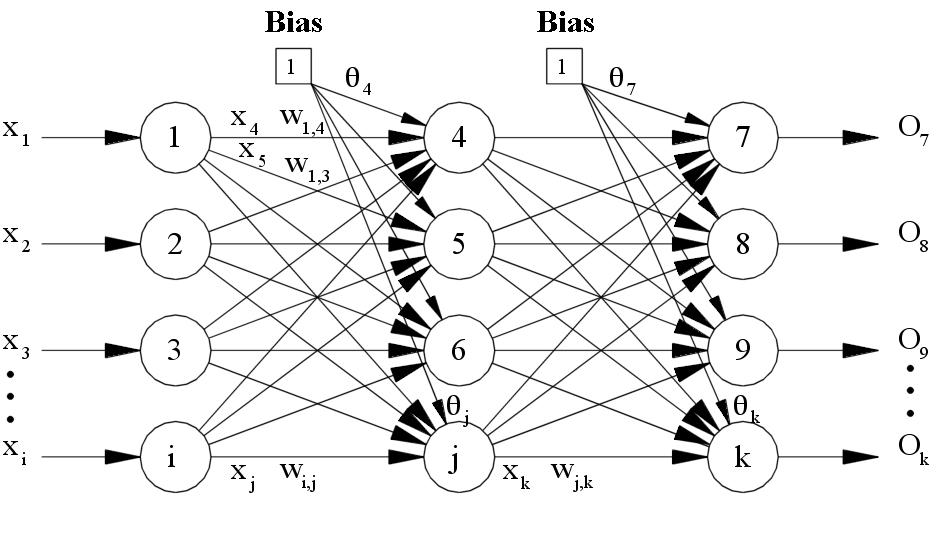
\includegraphics[width=0.75\columnwidth]{images/chap2/NeuralNetwork.jpg}
		\caption{A 2-layer Neural Network (one hidden layer of 4 neurons (or units) and one output layer with 2 neurons), and three inputs.}
		\label{chap2:neural_net}
		%https://www.researchgate.net/publication/302595416_Artificial_Neural_Network_Model_for_Rainfall-Runoff_-A_Case_Study
	\end{figure}
\end{center}
\footnotetext{Source: \url:{ https://devblogs.nvidia.com/mocha-jl-deep-learning-julia/}}
\vspace{-1cm}
Figure \ref{chap2:neural_net} represents a simple artificial neural network, where each circle is an artificial neuron, which is also called \textbf{Unit}, inward and outward arrows are the inputs and outputs of that neuron. The first layer where there is no input is called the \textbf{input layer}. Similarly, the last layer where there is no output is called the \textbf{output layer}. Layers that are either input or output are called \textbf{hidden layer}. In the figure, every neuron of one layer is connected to all neuron in the next layer, so it every layer is a “fully-connected layer”. A Network which only have \textbf{Fully-connected layer(s)} is also called as Multi Layer Perceptron (\textbf{MLP}).
\begin{center}
	\begin{figure}[H]
		\centering
		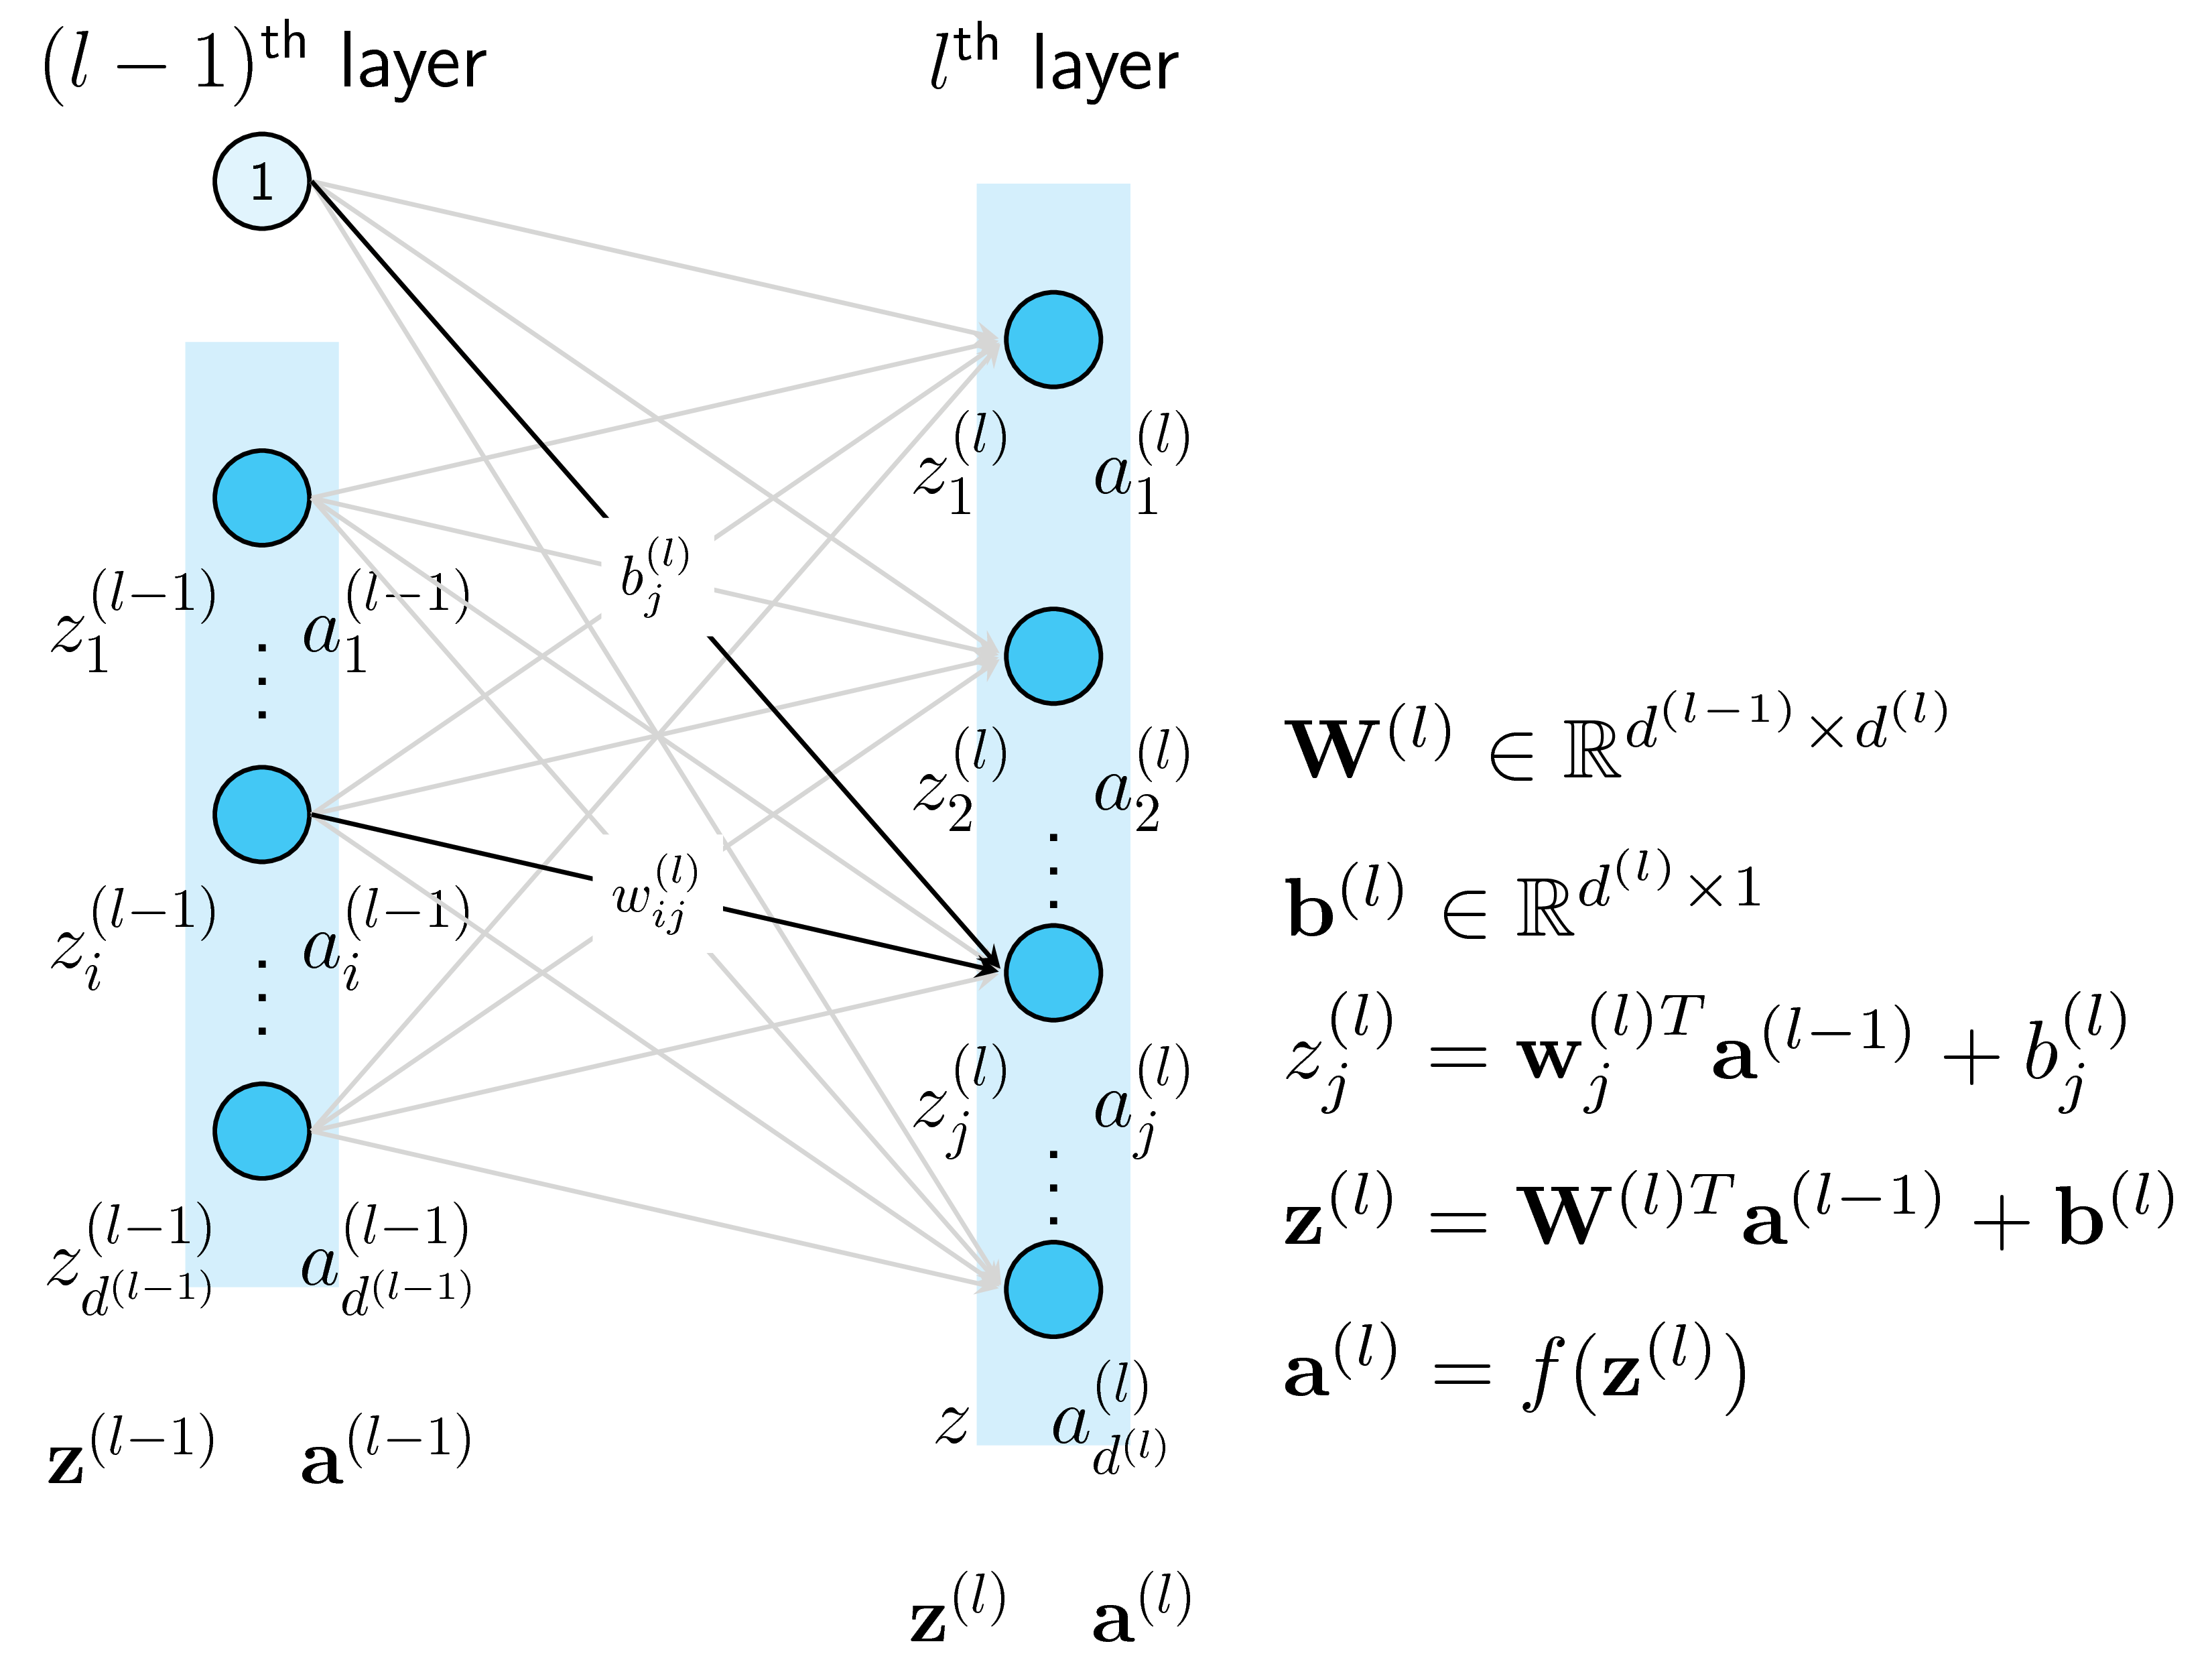
\includegraphics[width=0.75\columnwidth]{images/chap2/mlp_notation.png}
		\caption{Detail of processing in ANN}
		\label{chap2:neural_net_detail}
		%https://machinelearningcoban.com/2017/02/24/mlp/
	\end{figure}
\end{center}
\vspace{-1cm}
For more detail, in Figure \ref{chap2:neural_net_detail}. A blue circular node is called a \textbf{Unit}. Input of hidden layers is denoted by $z$, the output of each \textbf{Unit} is usually denoted by $a$
(shows the activation value, ie the value of each unit after we apply the activation function to $z$) The output of the $i^{th}$ unit in the $l^{th}$ layer is denoted by $a_{i}^{(l)}$, Suppose to add that the number of units in the $l^{th}$ layer) (without bias $b$) is $d^{(l)}$. The vector representing the output of the $l^{th}$ layer is denoted by $a^{(l)}$
There is $L$ of matrix in a FC with $L$ layers. These matrices are denoted by $W^{(l)}$,with $l = 1,2 ..., L$ where $W^{(l)}$ represents connections from layer $l-1$ to the $l^{th}$ layer (if we consider input layer is the layer $0$). More specifically, the element $w_{ij}^{(l)}$ represents the connection from the $i$ node of the second layer ($ l-1 $) to the node from $j$ of the $l^{th}$ layer. The biases of $(l)$ layer are denoted by $b^{(l)}$. These weights are denoted as in Figure \ref{chap2:neural_net_detail}. When optimizes an \textbf{MLP} for a certain work, these weights and these biases need to be found.If the weights and biases is set correctly, the \textbf{MLP} can be used to estimate numerous complex mathematical problems.\\
The set of weights and biases is denoted by $W$ and $b$ respectively.

\subsection{Activation Function}
Each output of a unit (except for input units) is calculated based on the formula:
\begin{center}
	$a_{i}^{(l)} = $ $f(w_{i}^{(l)T}a^{(l-1)} + b_{(i)}^{(l)} )$
\end{center}
In which $f()$ is a (nonlinear) activation function. In vector form, the above expression is written as:
\begin{center}
	$a_{i}^{(l)} = $ $f(W_{i}^{(l)T}a^{(l-1)} + b_{(i)}^{(l)} )$
\end{center}
When $f()$ activation is applied to a matrix (or vector), we understand that it is applied to each element of that matrix (element-wise operation). Then these components are rearranged in the correct order to get a matrix of the same size as the input matrix.
There are many non-linear functions can be used with neurons. Currently, there is no theory about the use of non-linear functions in any case, and the selection of suitable nonlinear functions for a particular task in the experiment. In nonlinear functions, the following functions are most commonly used: Tanh, Sigmoid, ReLU.
\begin{itemize}
	\item \textbf{Tanh}\\
	Tanh function has a formula:  $\tanh(x) = \frac{e^{2x-1}}{e^{2x+1}}$ has an S-shaped graph, and takes the value of x to [-1,1].
	\begin{center}
		\begin{figure}[H]
			\centering
			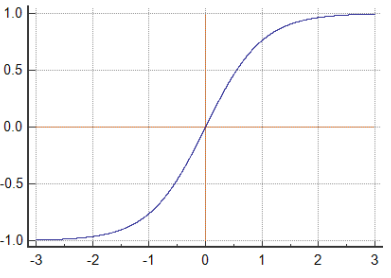
\includegraphics[width=0.5\columnwidth]{images/chap2/tanh.png}
			\caption{Tanh function graph}
			\label{chap2:tanh}
		\end{figure}
	\end{center}

	\item \textbf{Sigmoid}\\
	Sigmoid function has a formula: $ \sigma(x) = \frac{1}{1+\exp e^{-x}}$ has an S-shaped graph, and takes the value of x to [-1,1].
	\begin{center}
		\begin{figure}[H]
			\centering
			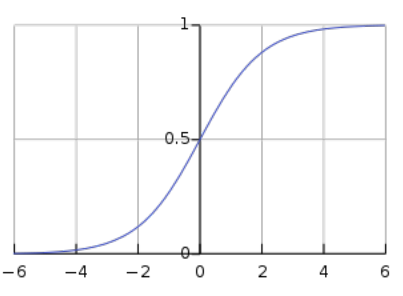
\includegraphics[width=0.5\columnwidth]{images/chap2/sigmoid.png}
			\caption{Sigmoid function graph}
			\label{chap2:sigmoid}
		\end{figure}
	\end{center}
	\item \textbf{ReLU}\\
	Rectified linear Unit is a simple nonlinear function but has very good results in experiments, it's has formula $ReLU(x) = max (0,x)$.
		\begin{center}
		\begin{figure}[H]
			\centering
			\includegraphics[width=0.5\columnwidth]{images/chap2/ReLU.png}
			\caption{ReLU function graph}
			\label{chap2:relu}
		\end{figure}
	\end{center}
\end{itemize}
\vspace{-1cm}
\subsection{Softmax}

With classification problems, the \textbf{Output layer} is often a \textbf{Softmax Regression} layer that calculates the probability that a data point falls into each class. Softmax has a simple formula:\\
\begin{center}
	$ softmax(x) = $\scalebox{1.4}{$\frac{e^{x_{j}}}{\sum\limits_{j=1}^k e^{x_{j}}} $}$, \forall X = [x_{1},x_{2},...x_{k}]$
\end{center}


\begin{center}
	\begin{figure}[H]
		\centering
		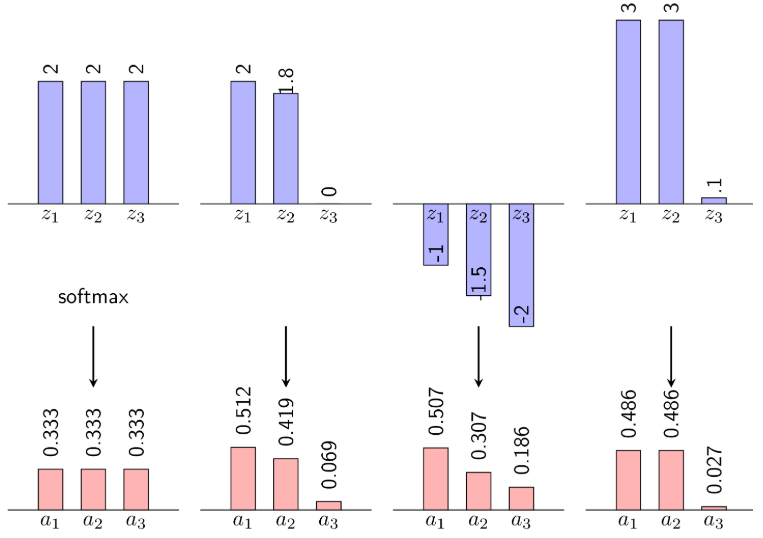
\includegraphics[width=0.75\columnwidth]{images/chap2/Softmax.png}
		\caption{Some examples of Softmax input and output}
		\label{chap2:softmax}
		%https://machinelearningcoban.com/2017/02/17/softmax/
	\end{figure}
\end{center}
\vspace{-1cm}
\subsection{Loss function}
When training an artificial neural network, the loss function needs to be defined, L ($\hat{y}, y$) showing the difference between the predicted $\hat{y}$ result and the correct value y. This function always has a non-negative value and is only 0 when $\hat{y}$ equals y.

The training process will be to adjust the model parameters (Weight W and bias b) so that the \textbf{Loss function} value is as small as possible.

A loss function is any function that takes two vectors and returns a scalar value. For optimization purposes, the loss function is often defined so that it is easy to calculate the derivative.

For multi-layer classification, the commonly used loss function is categorical cross-entropy
\textbf{Categorical cross-entropy} is used when expect outputs to be a probability.
With $y$ is one-hot encode vector representing the correct class of input and $\hat{y} = [\hat{y_1},\hat{y_2},..,\hat{y_n}$ is the output vector of the network has been transformed by Softmax function and can be considered as a representation of the first data in class $i: \hat{y} = P(y = i|x)$. Categorical cross-entropy measures the difference between $\hat{y}$ and $y$ distributions
\begin{center}
	$L_{cross-entropy}(\hat{y},\hat{y}) = - \sum\limits_{i}y_{i}\log(\hat{y}_{i})$
\end{center}
\subsection{Dropout}
Dropout \cite{Srivastava:2014:DSW:2627435.2670313} is a simple but effective method to reduce overfitting for neural network models.
At the output of each layer in the network, some neurons will be retained with the probability $p$, the remaining neurons are assigned a value of 0, during the back propagation, only the neurons are used to calculate derivative. Finally, in the validation process, we retain all neurons to produce predictable results
\begin{center}
	\begin{figure}[H]
		\centering
		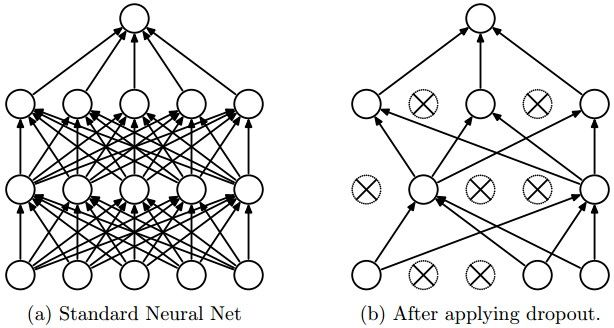
\includegraphics[width=0.75\columnwidth]{images/chap2/dropout.jpg}
		\caption{\textbf{Left:} Standard Neural Network with 2 hidden Layers. \textbf{Right:} An example of Dropout}
		%https://hackernoon.com/is-the-braess-paradox-related-to-dropout-in-neural-nets-270ecb97cdeb
		\label{chap2:dropout}
	\end{figure}
\end{center}
\vspace{-1cm}
\section{Convolution Neural Network (CNN)}
\subsection{Overview}
The CNN is inspired by the visual nerve system in animals, which is responsible for processing brain imaging data. Within this system, specific neurons only emit signals when a specific feature appear in the visual area. The human brain processes images through each layer with increasing complexity. The first layer distinguishes essential characteristics such as straight lines or curves. On the next layer, the brain will recognize the current arrangement of lines and colors that represent a dog or a cat. Similarly, CNN also processes images using multiple weight matrices called filters to detect features such as edges, lines... When going to higher layers, filters will be able to identify complex properties.

\subsection{Convolution Neural Network Architechture}
Simple architecture for Convolution Neural Network could be [INPUT - CONV - RELU - POOL - FC]. In more detail:

\begin{itemize}
	\item Input: [width-heigth-channel] for example in CIFAR -10 classifications, the input is [32x32x3] which hold the raw pixel values of the image, in this case, an image of width 32, height 32, and with three color channels Red, Blue, Green ( [32x32x3]).
	\item CONV layer is the most important layer, will compute the output of neurons that are connected to local regions in the input, the returned result could be [32x32x12] if 12 filters are decided to be used.
	\item RELU layer (Rectified linear unit) will apply an elements wise activation function (it is also the most commonly used activation function in deep learning models). The function returns 0 if it receives any negative input, but for any positive value x, it returns x back. F(x) = max(0,x).
	\item POOL (Pooling) layer will perform a downsampling operation along the spatial dimensions (Width, Height), result in volume such as [16 x 16 x 12].
	\item FC (Fully-connected) layer will compute the score of classes, resulting in a volume of size [1 x 1 x number of class] in Cifar-10, it returns [1x1x10].
\end{itemize}
By this way, CNN transforms the original image layer by layer from raw pixel values to the final class score. Note that some layers contain parameters, and others do not. For instance, CONV and FC layers contain not only the activation but also weight and the biases of the neurons. On the other hand, the RELU/POOL layers will implement a fixed function. The parameters in the CONV/FC layers will be trained with the gradient descent algorithm so that the class scores that the CNN computes are consistent with the labels in training set for each image.\\
\begin{center}
  \begin{figure}[H]
  \centering
  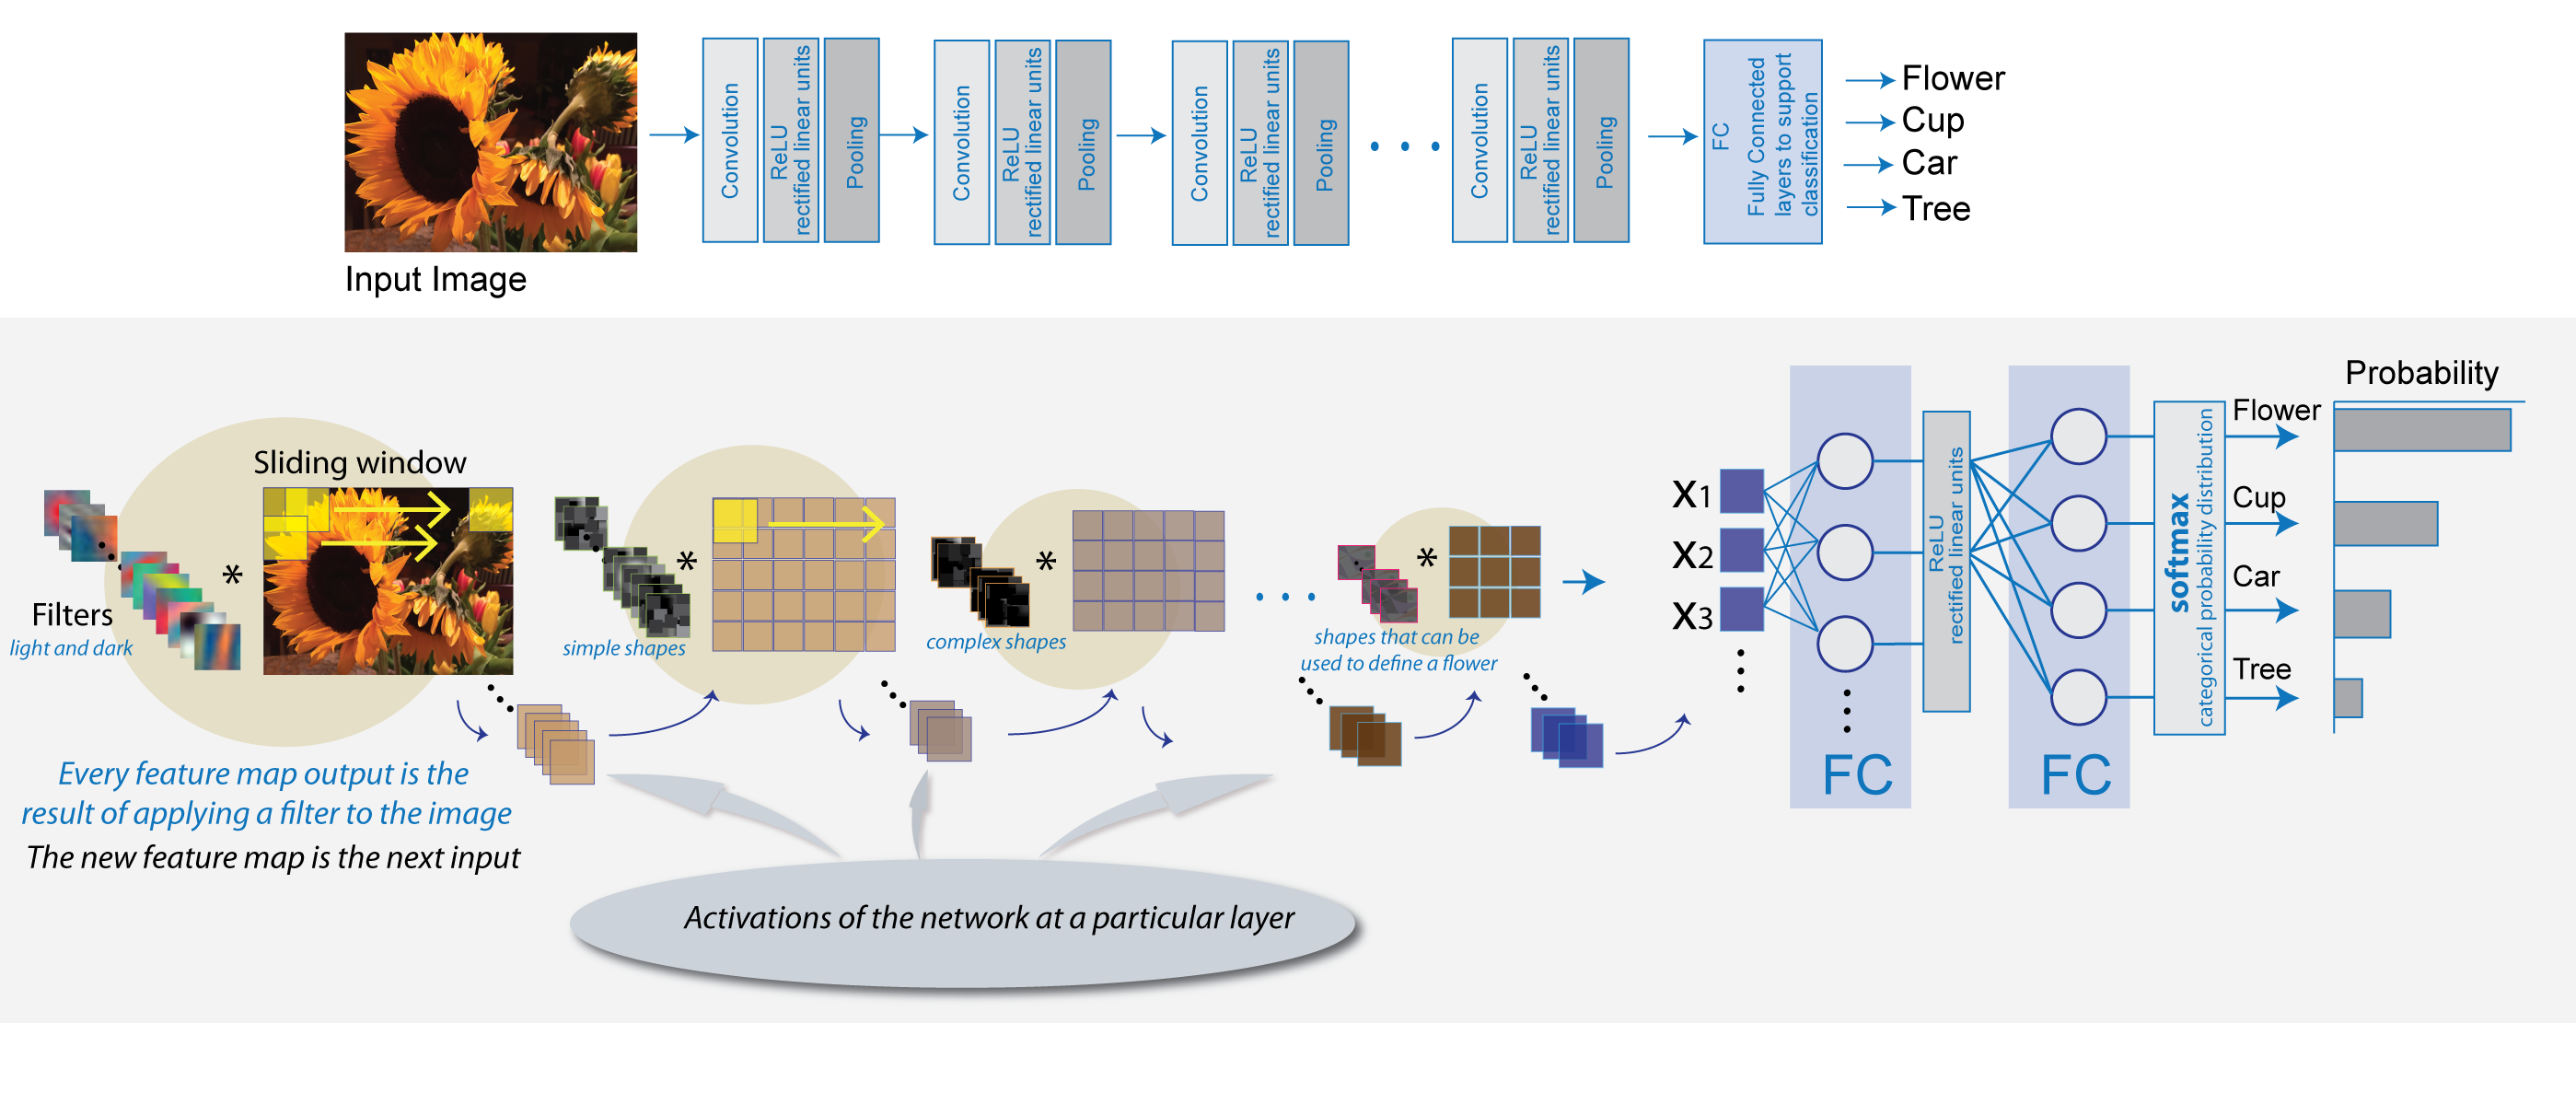
\includegraphics[width=1\columnwidth]{images/chap2/Intro_CNN.png}
  \caption{Simple Convolution Neural Network Architecture}
  \label{chap2:CNN arch}
  \end{figure}
\end{center}

\vspace{-1cm}
\subsection{Convolution Layer}
Convolution layer is the core building block of a Convolution Network that does the most critical computations in the Network.
\begin{itemize}
	\item Overview:\\ 
	The convolution layer's parameter consists of a set of learnable filters. Every filter is small spatially [ Width x Height], but extends through the full depth of the input volume (in standard image, the depth is equal 3). For example, a typical filter on the first layer of a CNN might have a size [5x5x3] (5 pixels width and height, and depth = 3). In the calculating process, slide each filter across the width and height of the input and compute dot-product between input and filter in every position. The result of dot-product is a 2-dimensional matrix called activation map of a filter. With layer has 12 filters, each of them produces one activation map, then stack these maps along the depth dimension and produce the output volume.
	\item Local Connectivity:\\
	When processing input which high-dimensional such as images, connect neurons to all previous neurons like Fully-connected layer is impractical, a number of parameters of the network must learn is massive (exploding hyperparameters). Alternately, each neuron is connected to only a local region of the input volume,the limit region of this connectivity is a hyperparameter called receptive field of the neuron (equivalently this is the size of the filter). The connections are local in space (along with width and height), but always full along the entire of the depth of the input volume.
	\begin{center}
		\begin{figure}[H]
			\centering
			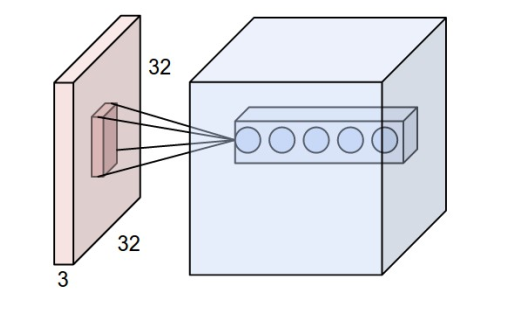
\includegraphics[width=1\columnwidth]{images/chap2/LocalConnectivity.png}
			\caption{Local connectivity in Convolution Neural Network}
			\label{chap2:LocalConnectivity}
		\end{figure}
	\end{center}
	\vspace{-1cm}
	\item Output volume: There is three hyperparameters affect the output volume: the depth, stride, and zero-padding.\\
	\begin{enumerate}
		\item Depth: Depth of output volume is corresponds to the number of filters used in the network. Each filter learning to look for something different in the input. For instance, with input is a raw image. First Conv Layer can learn a way to detect some primary attribute like edge, color or blobs … Set of neurons that are all looking at the same region of the input are called depth column (sometimes called fiber).\\
		\item Stride: stride is the step of filter over input. If stride is 1, a filter is moved 1 pixel per step, identical to stride equal 2 or 3. Therefore, this will produce smaller output volumes spatially ( smaller in Width and Height)
		\item Zero-Padding: Zero-padding is the number of line of Zero around the input volume, applying zero-padding allow us to control Height and Width of output volume (Commonly, it is used to preserve the spatial size of the input and output volume)
		
	\end{enumerate}
\end{itemize}
Output volume can be computed by using input volume size (W), the receptive field size of the Convolution Layer neurons (F), the stride value (S), and the amount of zero padding used (P) on the border. The formula for calculating how many neurons "fit" is given by:
\begin{center}
	\[ \scalebox{1.5}{$\frac{W_{1} - F + 2P }{S} + 1$} \]
\end{center}
For example, with input (W) = 7x7, filter (F) = 3x3, stride (F) = 1, Zero-padding 1, the output will be 5x5




\begin{center}
  \begin{figure}[H]
  \centering
  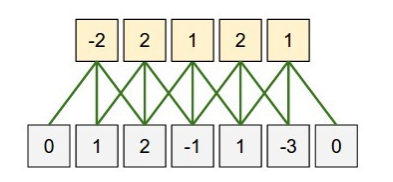
\includegraphics[width=1\columnwidth]{images/chap2/Output_volume_WSP.png}
  \caption{Output volume with F = 3, W = 5, S = 1 and Zero-Padding P = 1 }
  \label{chap2:Outputvolume_example}
  \end{figure}
\end{center}
\textbf{Summary Convolution Layer:}
\begin{itemize}
	\item Accept a volume size $W_{1}$ x $H_{1}$ x $D_{1}$ as input
	\item Requires four hyperparameters:
	\item Number of filter K
	\item Their spatial extent F 
	\item The stride S
	\item The amount of zero padding P
	\item Return an output with volume $W_{2}$ x $H_{2}$ x $D_{2}$ with:
	\begin{align*}
		W_{2} &= \frac{W_{1} - F + 2P }{S} + 1 \\
		H_{2} &= \frac{H_{1} - F + 2P }{S} + 1 \\
		D_{2} &= K
	\end{align*}
\end{itemize}

\subsection{Pooling Layer:}
Pooling Layer's function is to progressively reduce the spatial size of the representation to reduce the number of parameters and computation in the network, and control overfitting too. Pooling Layer operates independently on every depth slice of the input and resizes it spatially, using MAX, AVERAGE, SUM operation. The most common form is a pooling with MAX operation, filters of size 2x2 applied with a stride of 2, it will downsample every depth slice in the input by two along both width and height (depth is remaining).\\
\begin{center}
  \begin{figure}[H]
  \centering
  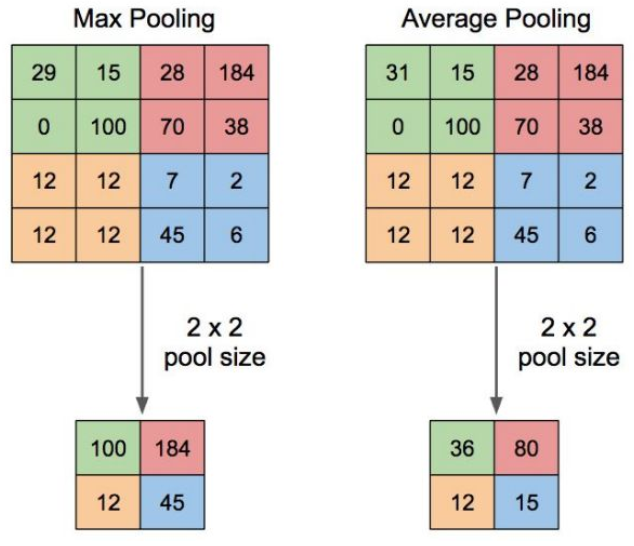
\includegraphics[width=1\columnwidth]{images/chap2/Pooling.png}
  \caption{Max Pooling and Average Pooling}
  \label{chap2:MaxPooling and Average Polling}
  \end{figure}
\end{center}

\textbf{Summary Pooling layer:}
\begin{itemize}
	\item Accept a volume size $W_{1}$ x $H_{1}$ x $D_{1}$ as input
	\item Require two hyperparameters:
	\item Their spatial extent F 
	\item The stride S
	\item Produces a volume of size $W_{2}$ x $H_{2}$ x $D_{2}$ with:
	\begin{align*}
	W_{2} &= \frac{W_{1} - F }{S} + 1\\
	H_{2} &= \frac{H_{1} - F }{S} + 1\\
	D_{2} &= D_{1}
	\end{align*}
	\item No parameter, because it computes a fixed function of the input\\
	\item Zero-Padding is unusable in pooling layer
\end{itemize}



\subsection{Fully-Connected Layer:}
Same as Fully Connected in ANN, neurons in a fully connected layer have full connections to all activation functions in the previous layer. 

\subsection{Some well-known CNN architecture:}
\textbf{LeNet (1998):} Yann LeCun developed LeNet first successful applications of Convolutional Network in the 1990s. LeNet is used to reading zip code, digits.
\begin{center}
  \begin{figure}[H]
  \centering
  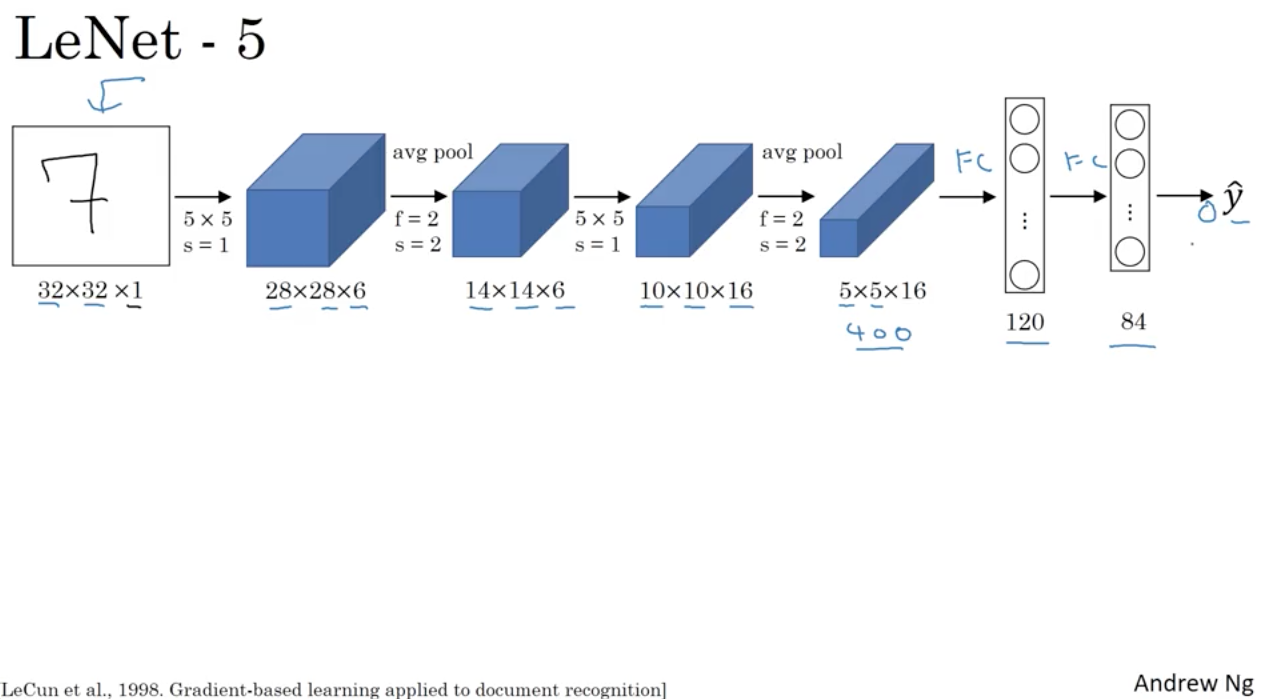
\includegraphics[width=1\columnwidth]{images/chap2/LeNet.png}
  \caption{LeNet Architecture}
  \label{chap2:WSP}
  \end{figure}
\end{center}
\vspace{-1cm}
\textbf{AlexNet (2012):} The first work that popularized Convolutional Networks in Computer Vision was the AlexNEt, developed by Alex Krizhevsky. The AlexNet got the first prize in ImageNet ILSVRC challenge 2012 and significantly outperformed the second (top 5 error of 16\% compared to runner-up with 26\% error).  
\begin{center}
  \begin{figure}[H]
  \centering
  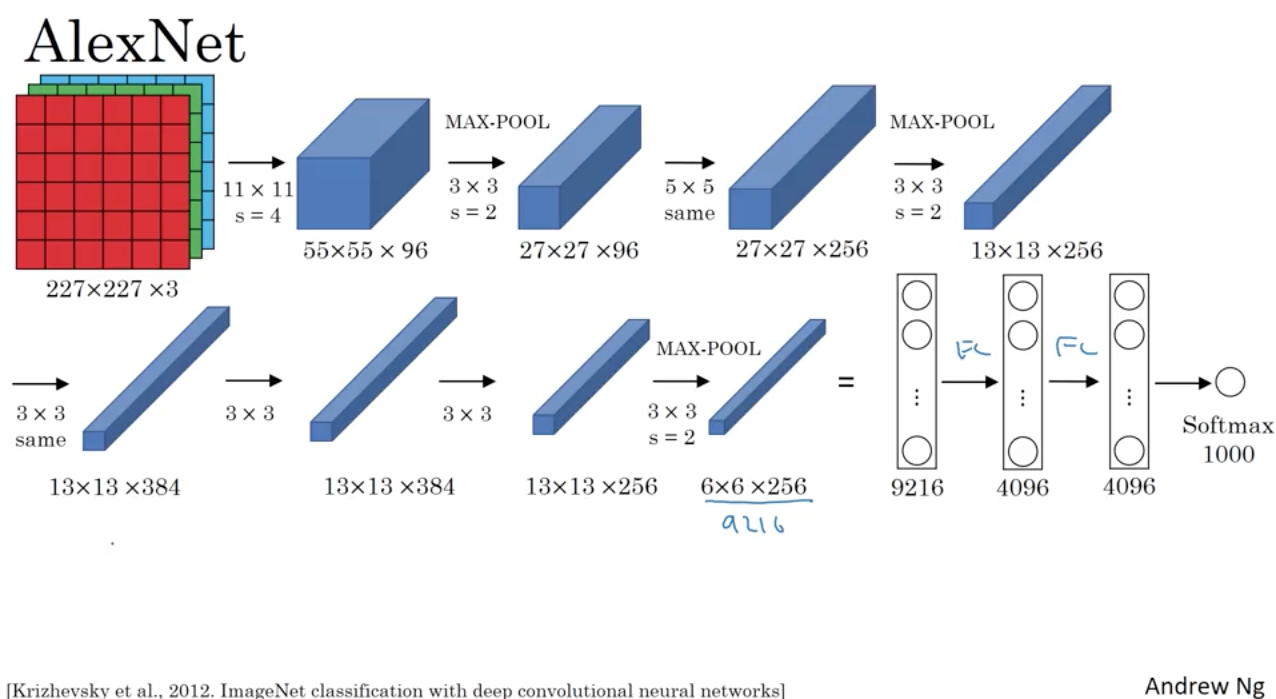
\includegraphics[width=1\columnwidth]{images/chap2/AlexNet.png}
  \caption{AlexNet Architecture}
  \label{chap2:WSP}
  \end{figure}
\end{center}
\vspace{-1cm}
\textbf{GoogLeNet (Inception - 2014):} The ILSVRC 2014 winner was a Convolutional Network from Szegedy from Google. Its the main contribution was the development of an Inception Module that dramatically reduced the number of parameters in the network (4 million, compared to AlexNet with 60M). Besides that, Average Pooling instead of Fully Connected at the top layer of the model, eliminating a large number of parameters that do not seem to matter much.
\begin{center}
  \begin{figure}[H]
  \centering
  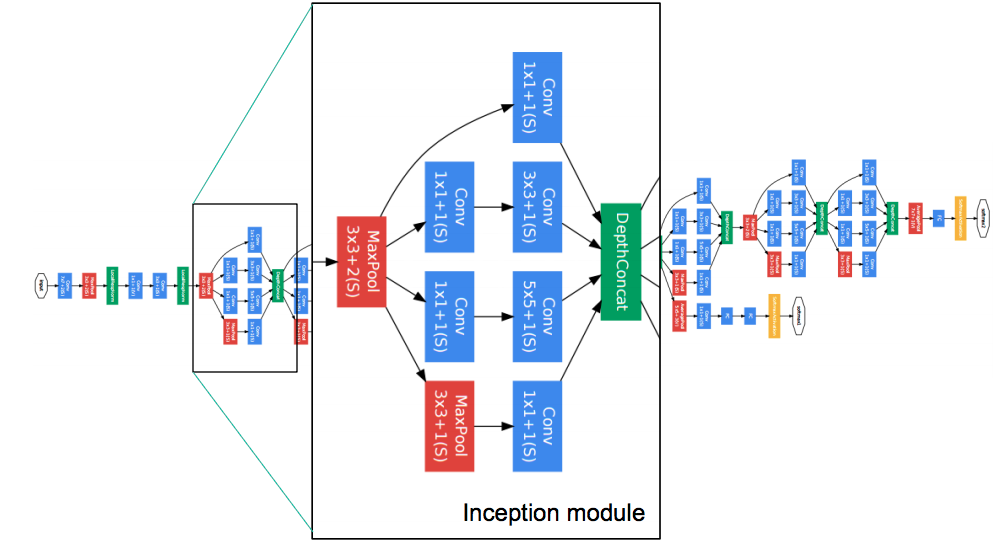
\includegraphics[width=1\columnwidth]{images/chap2/GoogleNet1.png}
  \caption{GoogleNet Architecture}
  \label{chap2:WSP}
  \end{figure}
\end{center}
\vspace{-1cm}
\textbf{VGGNet (2014):} The runner-up in ILSVRC 2014 is invented by VGG (Visual Geometry Group) from the University of Oxford. Its main contribution was in showing that depth of the network is a critical component for good performance. 
\begin{center}
  \begin{figure}[H]
  \centering
  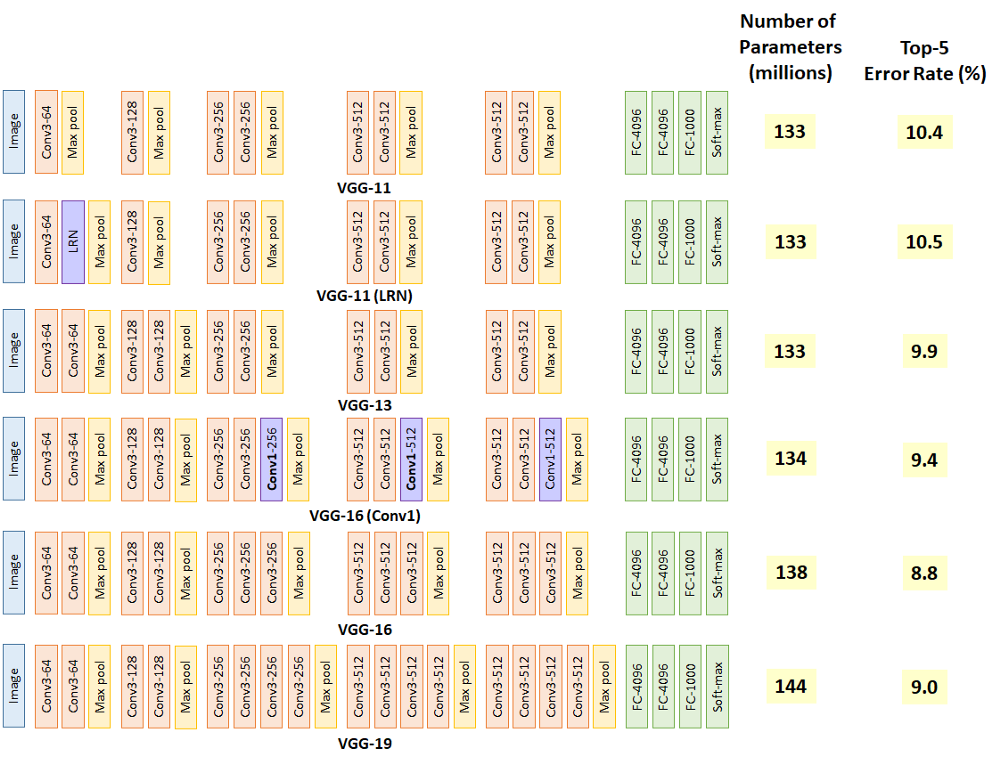
\includegraphics[width=1\columnwidth]{images/chap2/VGG_arch.png}
  \caption{VGG Architecture}
  \label{chap2:WSP}
  \end{figure}
\end{center}
\vspace{-1cm}
\textbf{ResNet(2015):} at the ILSVRC 2015, the so-called Residual Neural Network (ResNet) by Kaiming He introduced architecture with “skip connections” and features heavy batch normalization. Such skip connections are also known as gated units or gated recurrent units and have a strong similarity to recent successful elements applied in RNNs, this technique able to train a Neural Network with 152 layers while still having lower complexity than VGGNet. It achieves a top-5 error rate of 3.57\% which beats human-level performance on this dataset.
\begin{center}
  \begin{figure}[H]
  \centering
  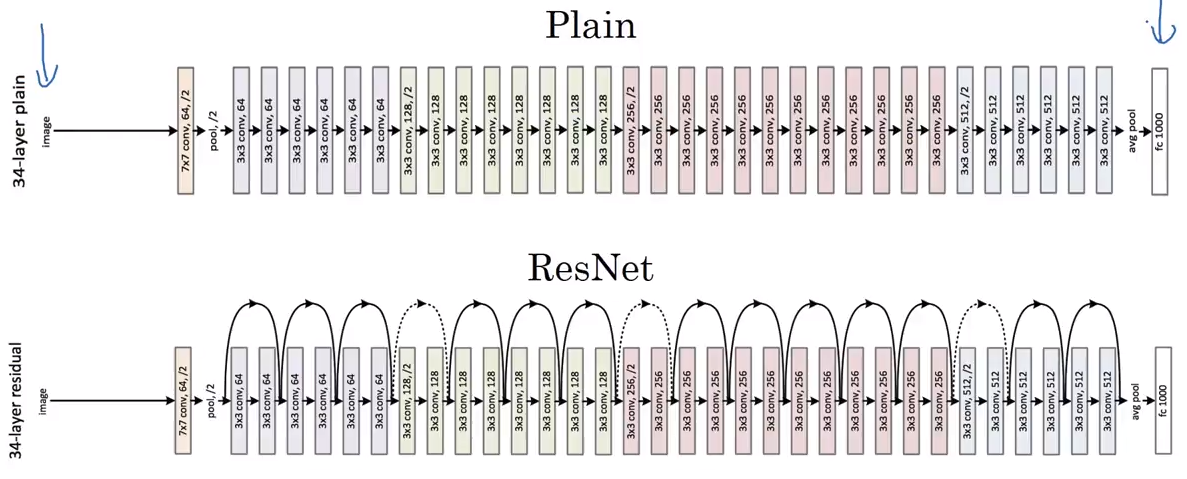
\includegraphics[width=1\columnwidth]{images/chap2/ResNet_Plain_Vs_Res.png}
  \caption{ResNet Architecture}
  \label{chap2:WSP}
  \end{figure}
\end{center}
\vspace{-1cm}
\subsection{Recurrent Neural Network (RNN)}
Human understanding does not come from scratch for every new input. When a man is reading a paragraph, his understanding of each word is based on his knowledge of previous words. That is why a human brain is persistent.\\
Traditional neural networks cannot do the task above. For example, if a traditional network wants to classify a frame in a video, it cannot use its reasoning of previous frames to help with the result of the current frame.\\
\textbf{Recurrent Neural Networks (RNN)} fix this issue by having loops within them, thus allowing information to be persistent. The remaining of this section is about the basics of RNN and \textbf{Long Short-Term Memory Network (LSTM)}, a variation of RNN designed to avoid the long-term dependencies problem of RNNs.


\subsubsection{Recurrent Neural Network - RNN}
\textbf{Recurrent Neural Network} is a type of neural network effective for processing sequential data. Recurrent Neural Network (RNN) was first introduced by Rumelhart et al. In 1986 \cite{Rumelhart:1986:PDP:104279} as a family of neural networks suitable for processing of chain data. Unlike others neural networks, which can only handle input of a given size, RNN can handle any input of any length, and it is possible to model the dependency of the latter component. With preceding components in the output. First, the RNN stores a hidden state vector that is updated at each processing step (timestep) based on the value of this vector at the pre-processing stage and the value of the input component at this step. Second, the rules for hidden status updates, expressed through a set of corresponding functions and weights, are shared between processing steps. These features allow the RNN network to be generalizable even to any size input chain and have achieved the best results in processing string data such as text and sound.
Let x = $[x_{0}, x_{1}, ..., x_{n}]$ be an input sequence of $n + 1$ components with each component $x_{t}$ $(t = 0..n)$ is a vector of a certain size. Let $h_{t}$, $y_{t}$ denote the latent state and output of RNN in step t. An original RNN (Vanilla RNN) is represented by the following mathematical formula:
\begin{align}
h_{o} &= \sigma_{h}(W_{xh}x_{t})\\
h_{t} &= \sigma_{h}(W_{hh}h_{t-1} + W_{xh}x_{t})\\
y_{t} &= \sigma_{t}(W_{hy}h_{t})
\end{align}
In the above formula, $W_{hh}, W_{xh}$ and $W_{hy}$ are respectively the weight matrices between $h_{t-1}$ and $h_{t}, x_{t}$ and $h_{t}, h_{t}$ and $y_{t}$. $\sigma_{h}$ and $\sigma_{y}$ are activation functions, where the $\tanh$ function is usually used for $\sigma_{h}$.
\subsubsection{Long Short-Term Memory - LSTM}

\textbf{Long Short-Term Memory (LSTM)} was first introduced in 1997 by Hochreiter and Schmidhuber. LSTM is designed to handle Vanishing/Exploding Gradients problem through a method known as a gating mechanism. To understand what a gateway is, first look at how the LSTM works. Vector hidden state in LSTM network is calculated through the following formula:

\begin{align}
i &= \sigma ( W_{xi}x_{t} + W _{hi}h _{t-1} + b _{i}) \\
f &= \sigma(W_{xf}x_{t} + W_{hf}h_{t-1} + b_{f}) \\
o &= \sigma(W_{xo}x_{t} + W_{ho}h_{t-1} + b_{o})	\\
g &= \tanh (W_{xg}x_{t} + W_{hg}h_{t-1} + b_{g})	\\
c_{t} &= c_{t-1} \circ f+ g \circ I	\\
h_{t} &= \tanh(c_{t}) \circ o
\end{align}
\begin{center}
  \begin{figure}[H]
  \centering
  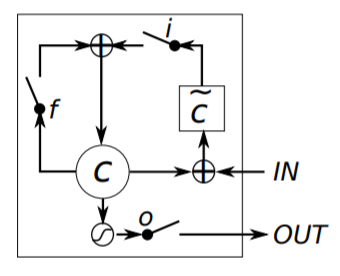
\includegraphics[width=0.5\columnwidth]{images/chap2/LSTM.png}
  \caption{Long Short-Term Memory cell \cite{DBLP:journals/corr/DonahueHGRVSD14}}
  \label{chap2:WSP}
  \end{figure}
\end{center}
\vspace{-1cm}
In the above formulas:

$i$, $f$ and $o$ are respectively called \textbf{input gate}, \textbf{forget gate} and \textbf{output gate}. These gate have the same formula that is based on the input $x_{t}$ at the current step and the $h_{t-1}$ state of the previous step, but has different weighting matrices. These values are called $Gate$ because they have a trigger function of \textbf{Sigmoid} so that the value is always in the range [0, 1]. Moreover, by executing \textbf{Hadamard multiplication} (by multiplying the respective elements of the two matrices of the same size) between this and another vector of the same size, then determine the amount of information that this vector allows to pass through. The \textbf{input gate} specifies the amount of new information that is passed, this new information is calculated from the input component of the current step and the hidden state of the previous step. The \textbf{forget gate} specifies the amount of information the hidden state of the previous step is allowed to pass through. Finally, the \textbf{output gate} determines the amount of information from the inner state that is taken to the next step and the higher layers in the model. All ports are equal in size to the size of the hidden state vector.
\begin{center}
  \begin{figure}[H]
  \centering
  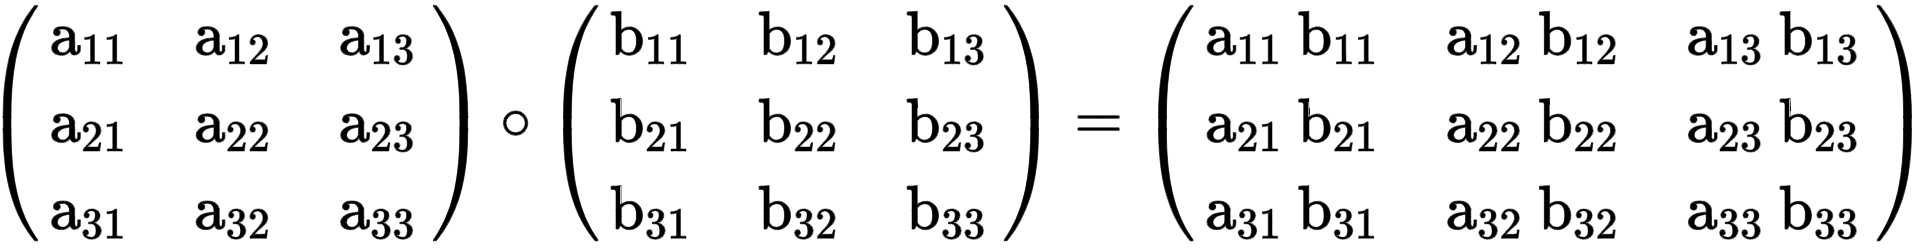
\includegraphics[width=0.8\columnwidth]{images/chap2/Hadamard.png}
  \caption{Hadamard multiplication}
  \label{chap2:WSP}
  \end{figure}
\end{center}

$g$ contains the combination of the hidden state of the previous step and the input component of the current step. In the pure RNN (Vanilla RNN), $g$ will be considered a new hidden state of the model. In the LSTM, the input gate will determine how much information from $g$ is used in the new hidden state.

$c_{t}$ is the internal memory of one unit. This is the memory combination between the memory value in the previous step $c_{t-1}$, multiplied by the \textbf{forget gate} and the value of $g$ multiplied by the input gate. So it can understand how internal memory is calculated by determining how much memory information is retained and how much information is added.

With the value of internal memory ($c_{t}$), it calculate the hidden state vector value by performing the \textbf{Hadamard multiplication} to the output gate ($o$) because not all of the internal memory values are related to the back-end layers, model or hidden state value of the next step



%\section{Face recognition}
%\section{Action recognition}
%\section{Cloud computing}


\cleardoublepage

\chapter{PROPOSED SOLUTION}
\label{chap:solution}




\cleardoublepage

\chapter{SYSTEM DESIGN AND IMPLEMENTATION}
\label{chap:caseFarming}
\paragraph{Chương 3} sẽ giới thiệu về giải pháp đề xuất của nhóm để giải quyết bài toán nhận diện trái trái bưởi.


\section{Design}
\subsection{Whole system design}
\subsection{Crowd-sourcing system design}
\subsection{Analysis system design}
\section{Implementation}
\subsection{Crowd-sourcing system implementation}
\subsection{Analysis system implementation}



\cleardoublepage

\chapter{EVALUATION}
\label{conclusion}
\paragraph{Chapter 5}will present the process of evaluating the effectiveness of the whole system and its features. At the same time, self-assessment of the work done by the group, from which the development direction of the topic

\section{Evaluation metric}
\section{Result}



\cleardoublepage

\chapter{CONCLUSION AND FURTHER DEVELOPMENT}

\section{Accomplishment}
Through the development of this thesis, the following accomplishments are achieved:
\begin{enumerate}
    \item Research and propose a model for analyzing video data. The problem of analyzing videos is treated as a video classification problem. This thesis proposes using a model containing a pretrained CNN for features extraction followed by LSTMs for sequence prediction and had moderate success.
    \item Build a system to collect data using the crowdsourcing model. This system has the form of a social media website. This website allows users to interact with each other and contribute labels to create labeled data for other purposes.
    \item Develop a UI to interact with users using modern HTML5. This UI support many platforms such as mobile and desktop.
\end{enumerate}


\section{Limitation}
There are some limitations of the system to be improved upon, which will be discussed in this section.
\subsection{Social media website}
\begin{enumerate}

\item Current way of deciding final label for a video is too simple.
\item There is no method to attract users and encourage users to label yet.
\item The system has a small number of users, so there are potential bugs to be undiscovered.
\item There are not many interactions between users, compare to typical social media websites. 
\item The system does not concern with privacy.
 
\end{enumerate}
\subsection{Data analysis modules}
\begin{enumerate}

\item Although the results of the classifier are positive, it is only tested on a small amount of data. There is not enough real data to train and test the video classification model so it cannot be used to classify real data yet.
\item There are not enough resources: Fund, hardware, ...s

\end{enumerate}
\section{Further development}
To fix above short-comings, some of the following improvements are proposed:
\subsection{Social media website}\begin{enumerate}
\item Implementing a rewarding system to attract users and encourage users to label video. Users earn points by creating posts and labeling video. Points are used to exchanged for rewards such as voucher, gift card, ...
\item Implement more features, so that the platform is more complete.
\item Improve method to decide the final label of videos.
\end{enumerate}
\subsection{Data analysis modules}
\begin{enumerate}
\item Collect more real data to train the model so that it becomes more accurate.
\item Optimize hyperparameters of the model to increase accuracy.

\end{enumerate}



\cleardoublepage

\chapter{REFERENCES}

\cleardoublepage

\appendix

\chapter{INSTALLATION}
\section{Prerequisite}
\tocless\subsection{Node.js}
\begin{enumerate}
	\item Download Node.js installer from its official download page (\href{https://nodejs.org/en/download/}{https://nodejs.org/en/download/})
	      \begin{center}
	      	\begin{figure}[H]
	      		\centering
	      		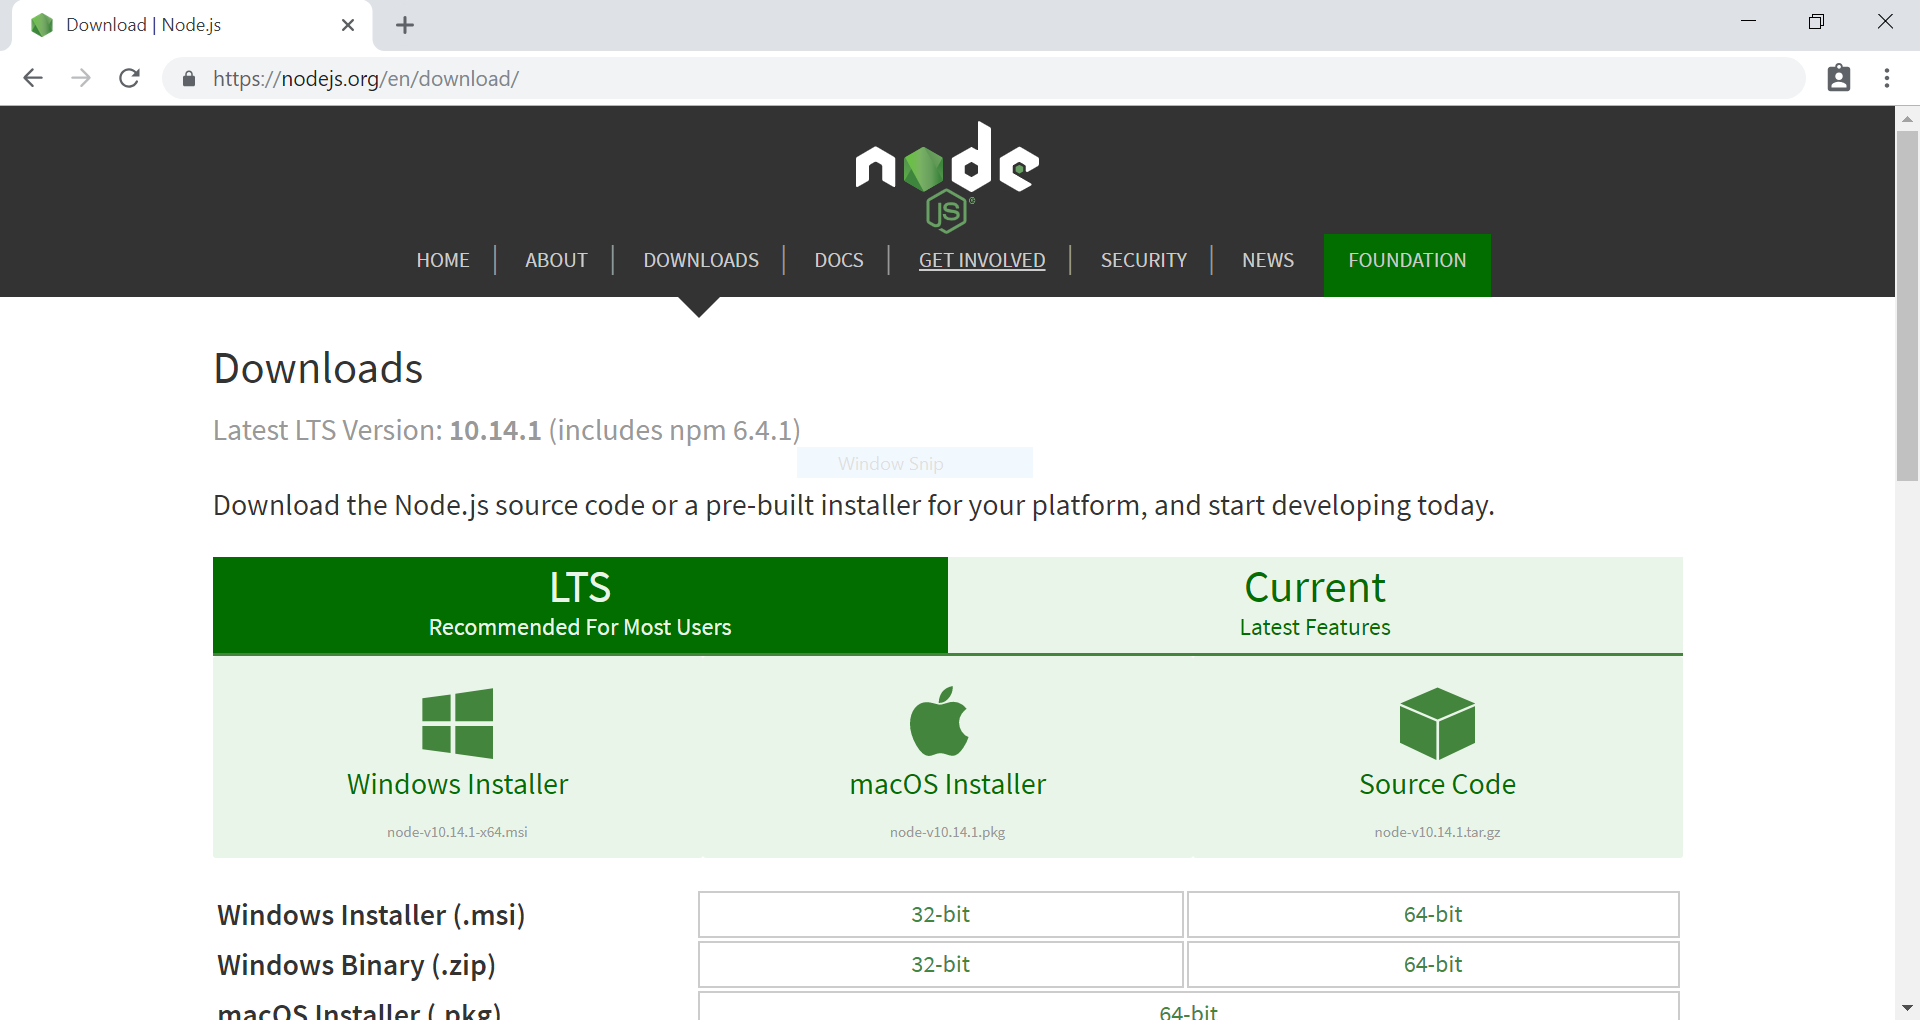
\includegraphics[width=0.6\columnwidth]{images/appendixA/Nodejs-download-page.PNG}
	      		\footcaption{Node.js official download page}
	      	\end{figure}
	      \end{center}
	      \footnotetext{Source: \url{https://nodejs.org/en/download/}} 
	\item Follow the instruction of setup wizard and install Node.js
	      \begin{center}
	      	\begin{figure}[H]
	      		\centering
	      		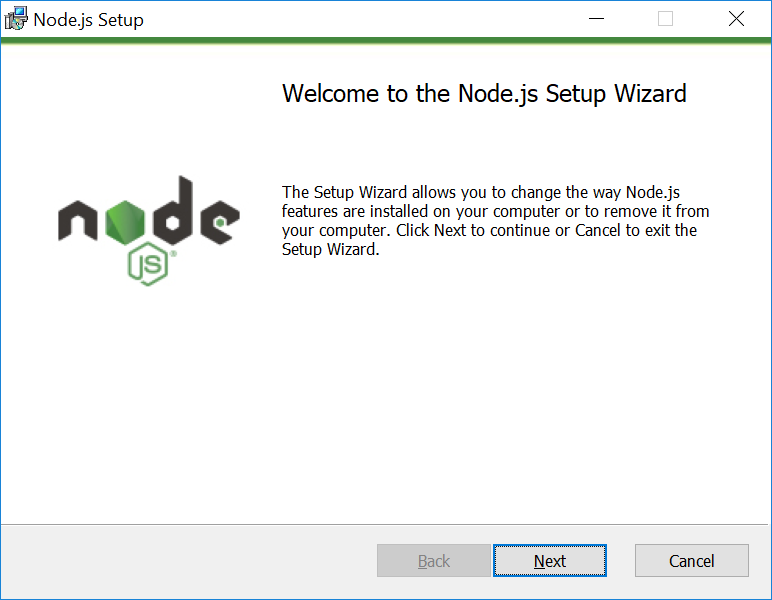
\includegraphics[width=0.6\columnwidth]{images/appendixA/Nodejs-setup.PNG}
	      		\footcaption{Node.js Setup Wizard}
	      	\end{figure}
	      \end{center}
	      \footnotetext{Source: Node.js Setup Wizard} 
	\item To verify installation, open \textit{Window Command Prompt} and enter following command: \verb+node -v+
	      \begin{center}
	      	\begin{figure}[H]
	      		\centering
	      		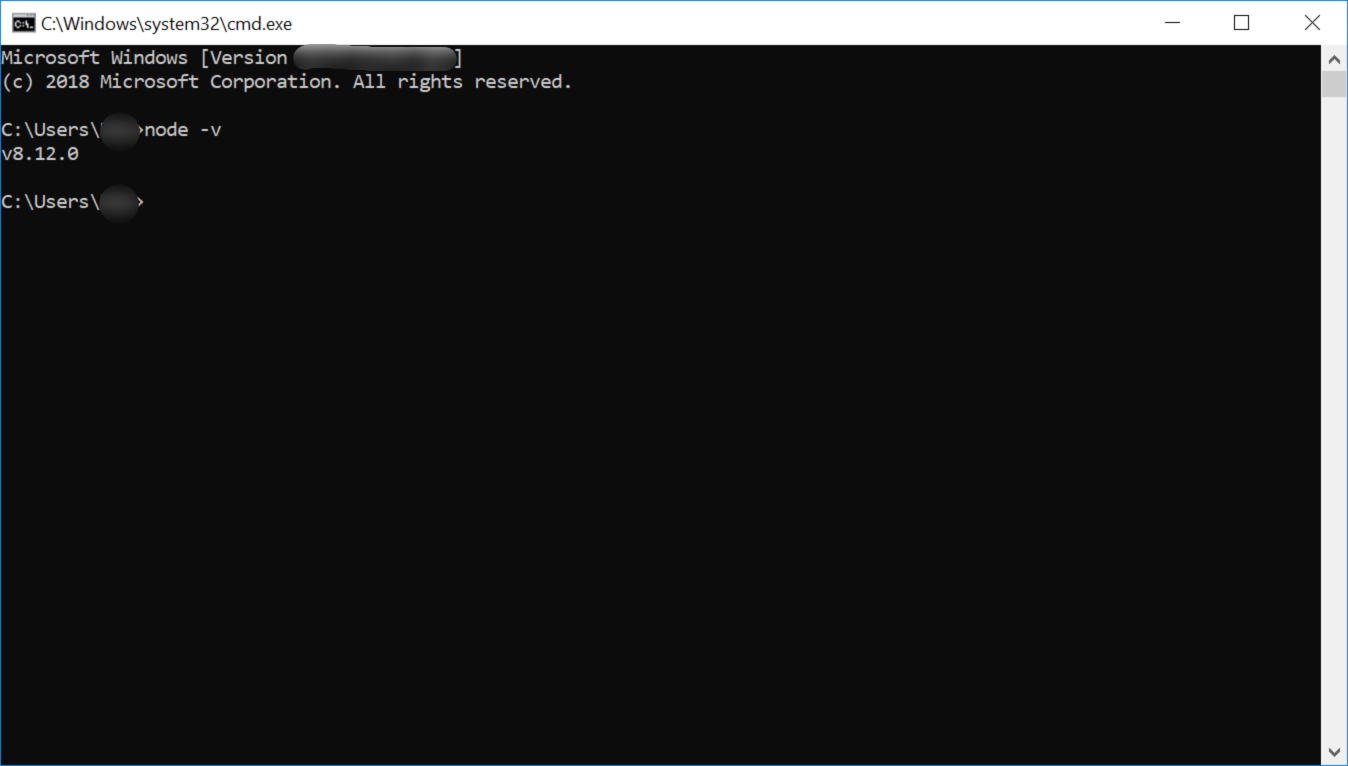
\includegraphics[width=0.6\columnwidth]{images/appendixA/Nodejs-verify-install.PNG}
	      		\footcaption{Node.js installation verification}
	      	\end{figure}
	      \end{center}
	      \footnotetext{Source: Window Command Prompt} 
\end{enumerate}
\tocless\subsection{Google Cloud Platform}
\begin{enumerate}
	\item Create an account and a new project on \textit{Google Cloud Platform} from \href{https://cloud.google.com/}{https://cloud.google.com/}
	      \begin{center}
	      	\begin{figure}[H]
	      		\centering
	      		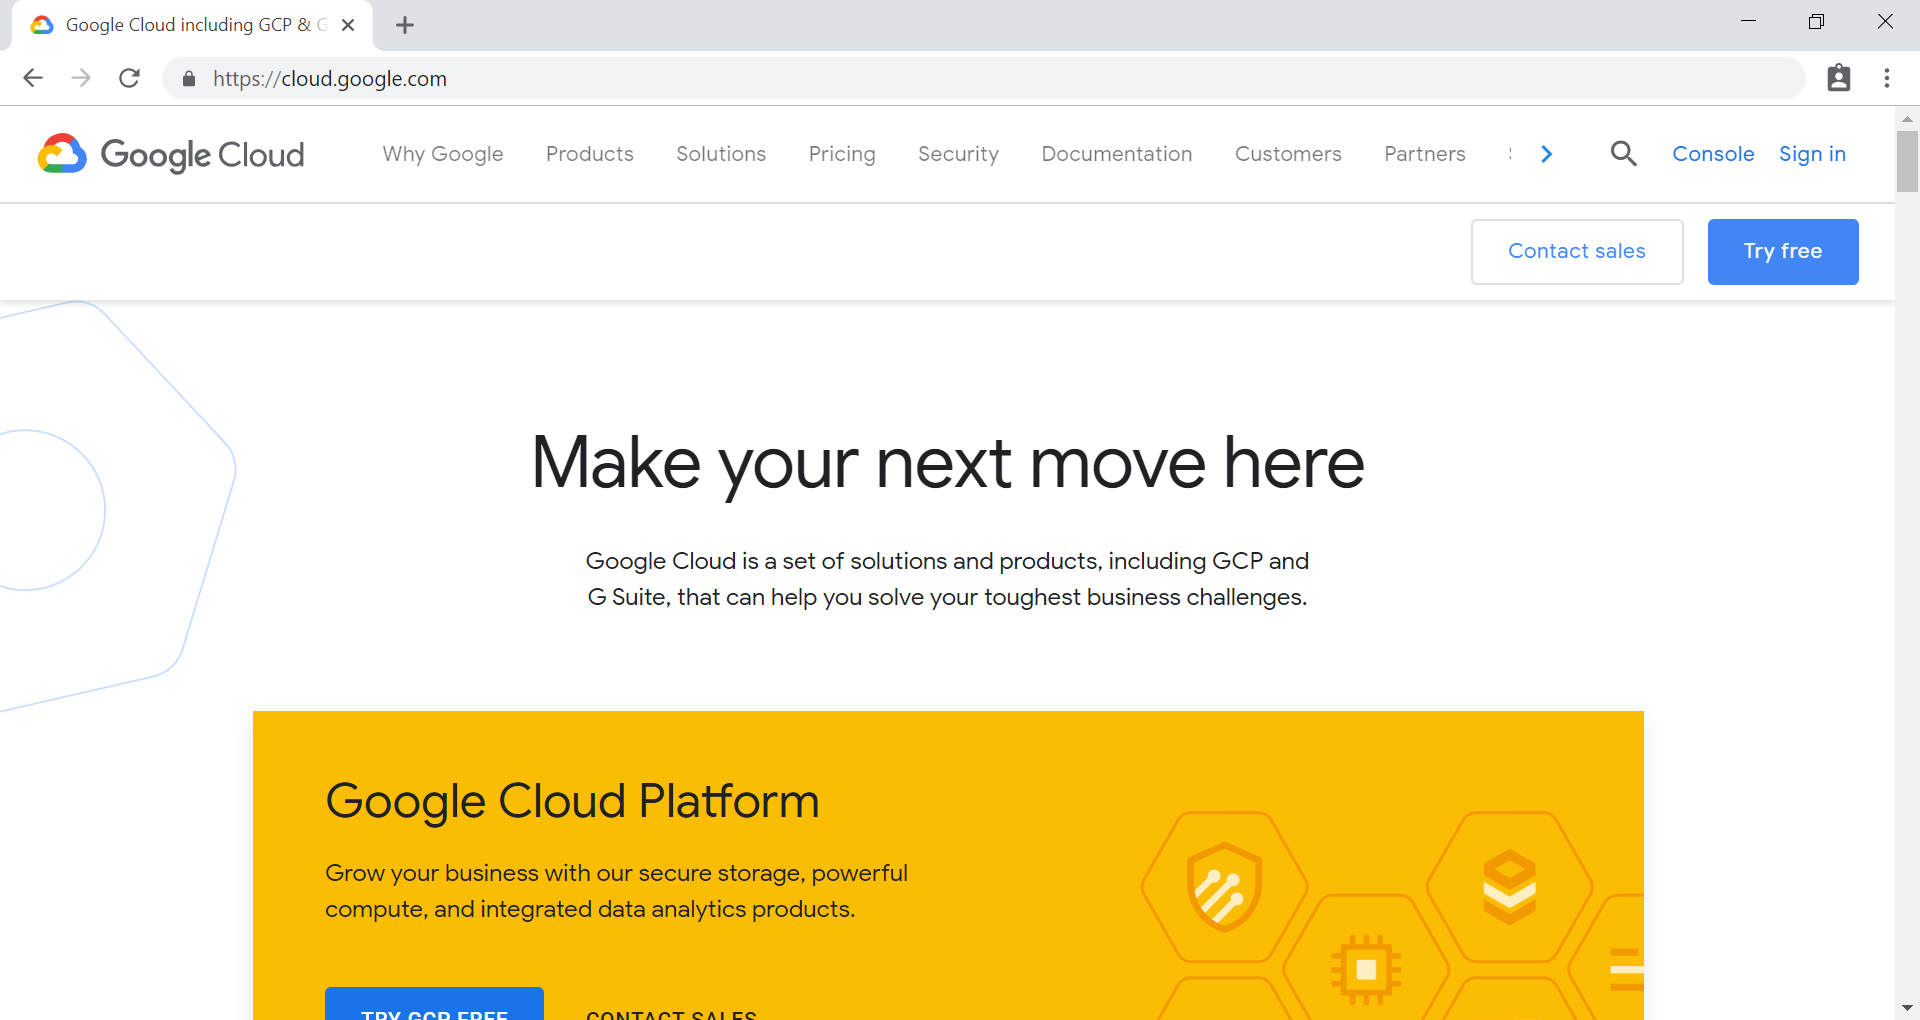
\includegraphics[width=0.6\columnwidth]{images/appendixA/GCP-homepage.PNG}
	      		\footcaption{Google Cloud Platform homepage}
	      	\end{figure}
	      \end{center}
	      \begin{center}
	      	\begin{figure}[H]
	      		\centering
	      		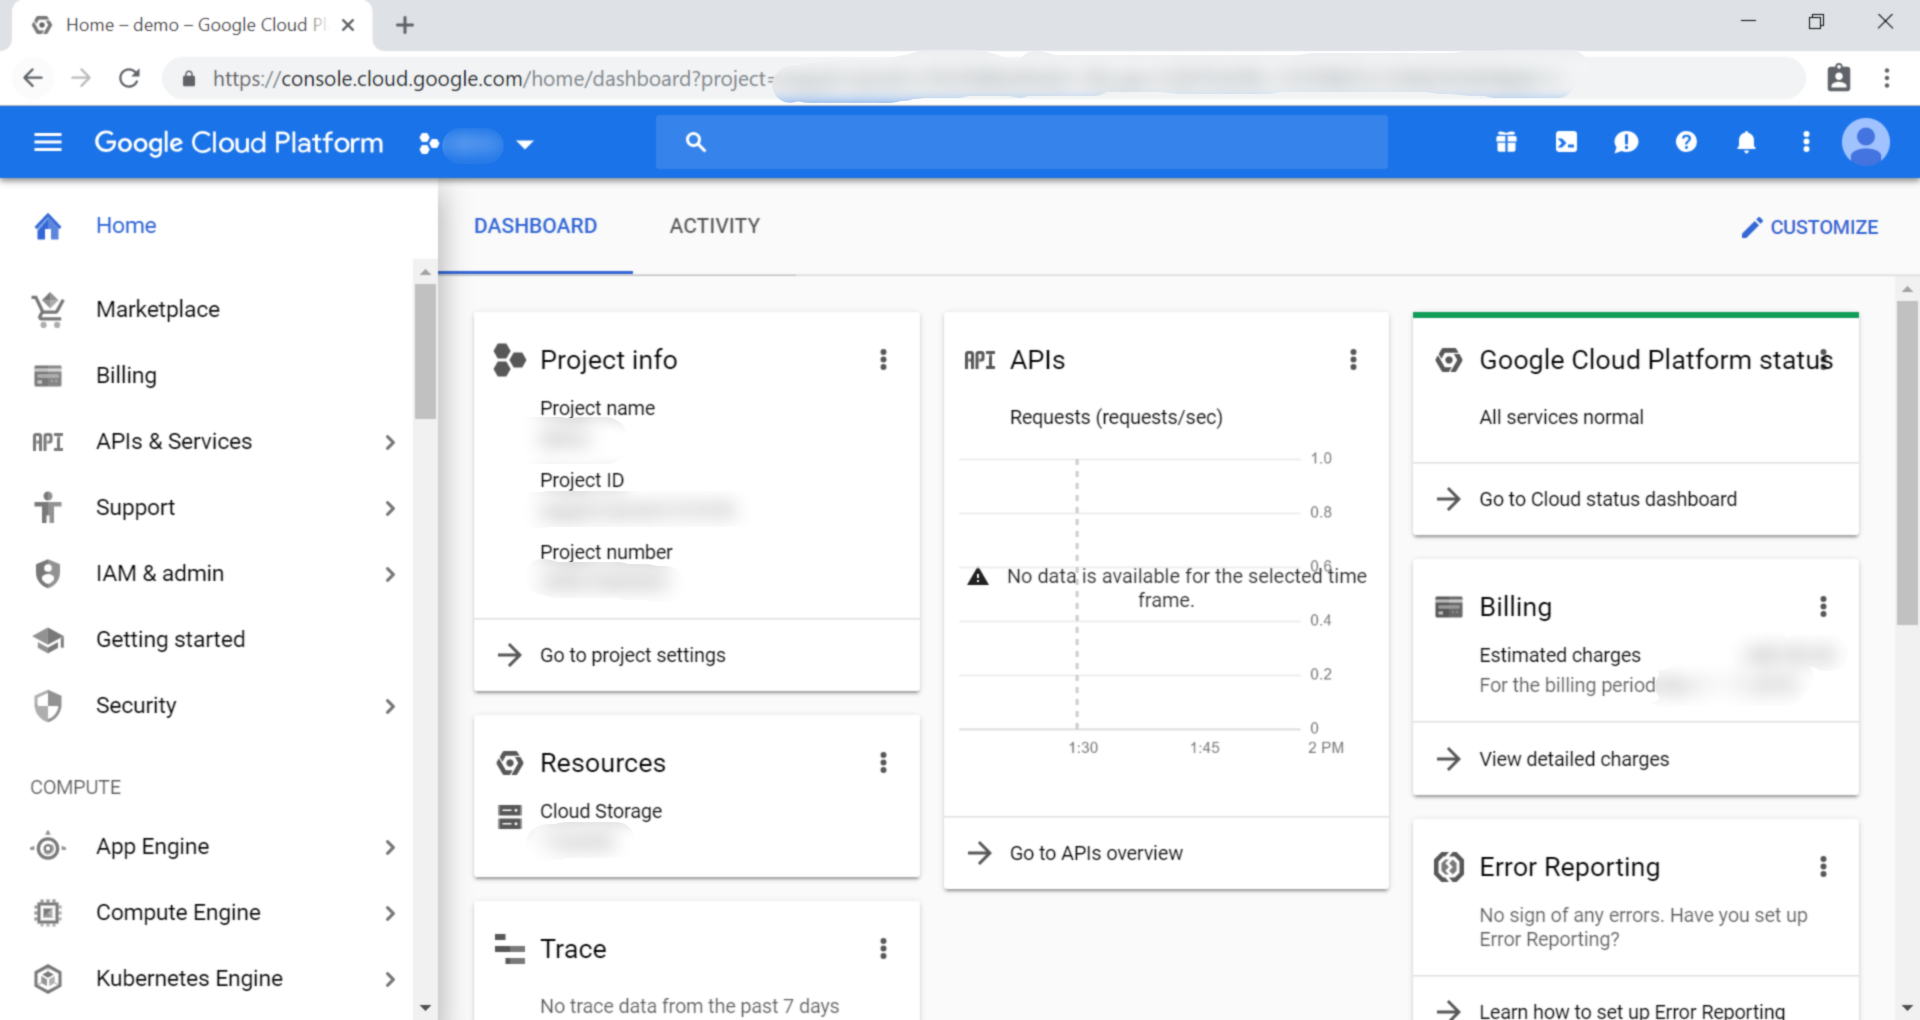
\includegraphics[width=0.6\columnwidth]{images/appendixA/GCP-console.PNG}
	      		\footcaption{Google Cloud Platform console}
	      	\end{figure}
	      \end{center}
	      \footnotetext{Source: \url{https://cloud.google.com/}} 
	\item Create \textit{Google Cloud Storage Bucket}. From the console, open navigation menu, and select \textit{Storage}
	      \begin{center}
	      	\begin{figure}[H]
	      		\centering
	      		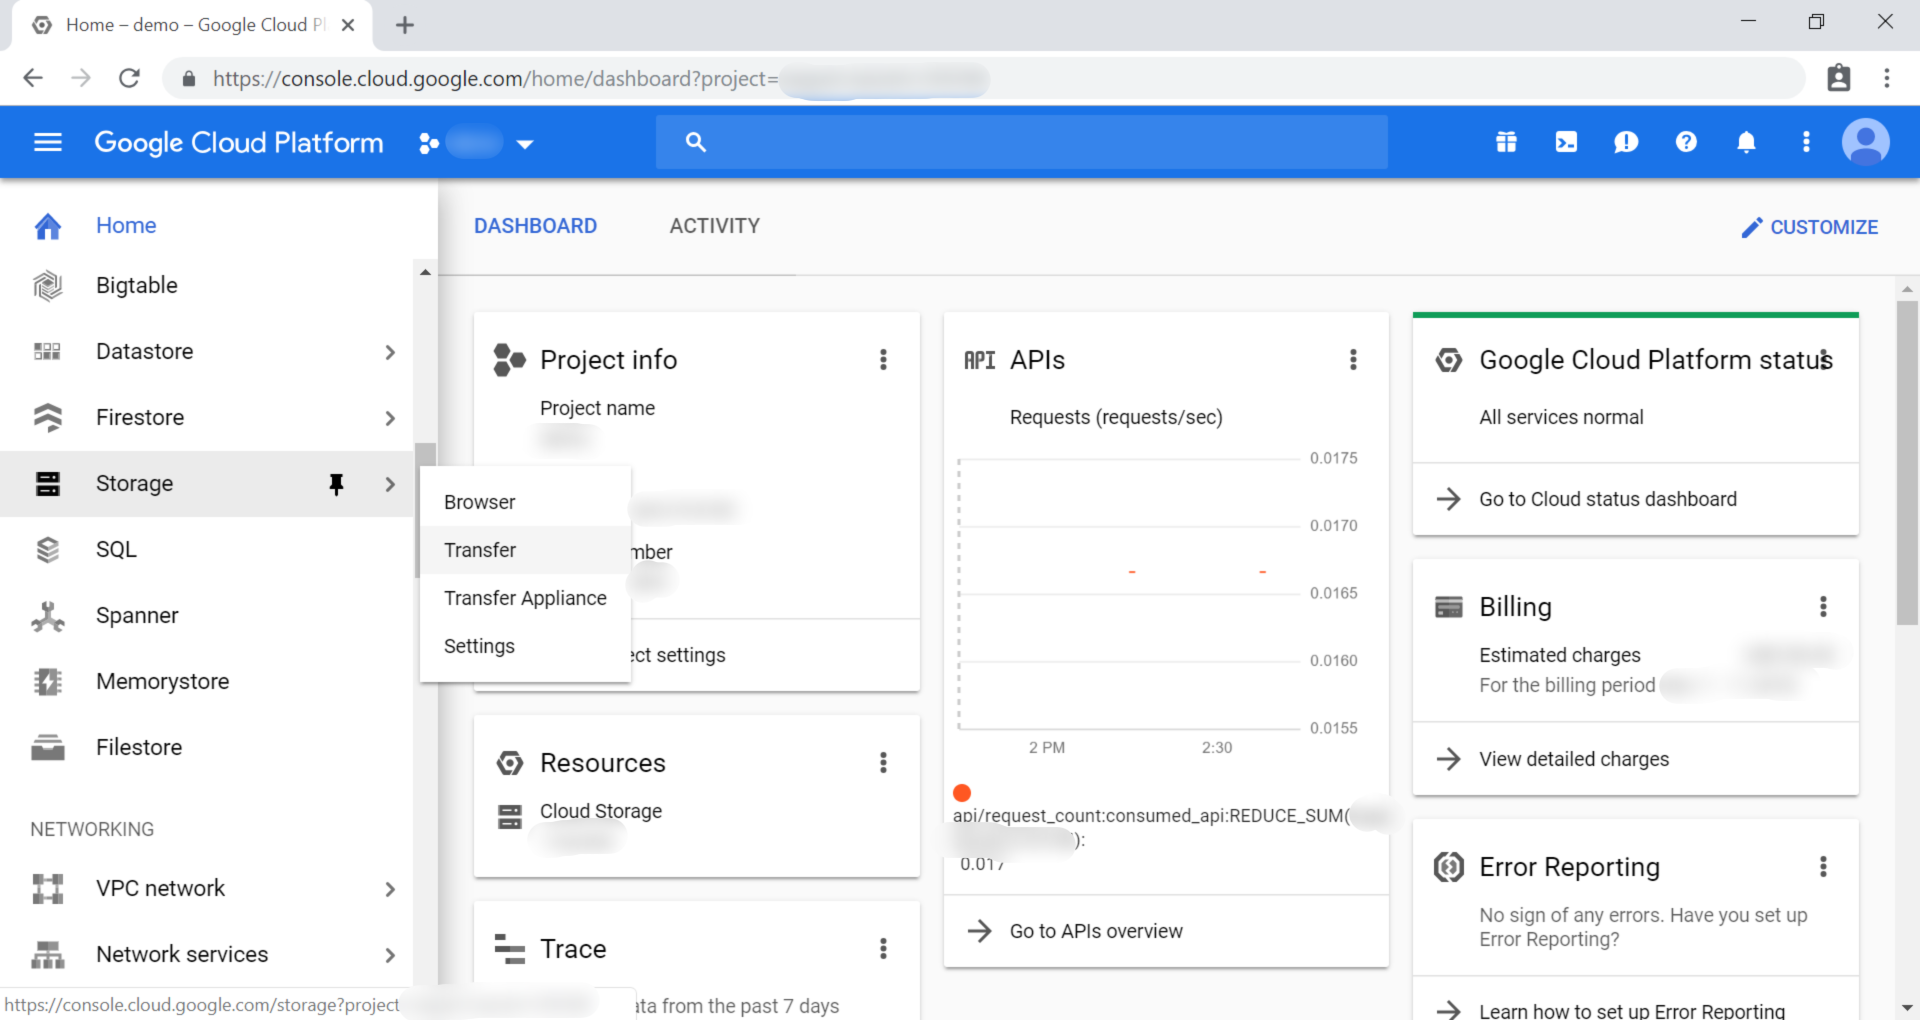
\includegraphics[width=0.6\columnwidth]{images/appendixA/GCP-navigate-Storage.PNG}
	      		\footcaption{Google Cloud Platform: Navigation Menu > Storage}
	      	\end{figure}
	      \end{center}
	      \footnotetext{Source: \url{https://cloud.google.com/}} 
	\item Click \textit{Create bucket} button and provide required information
	      \begin{center}
	      	\begin{figure}[H]
	      		\centering
	      		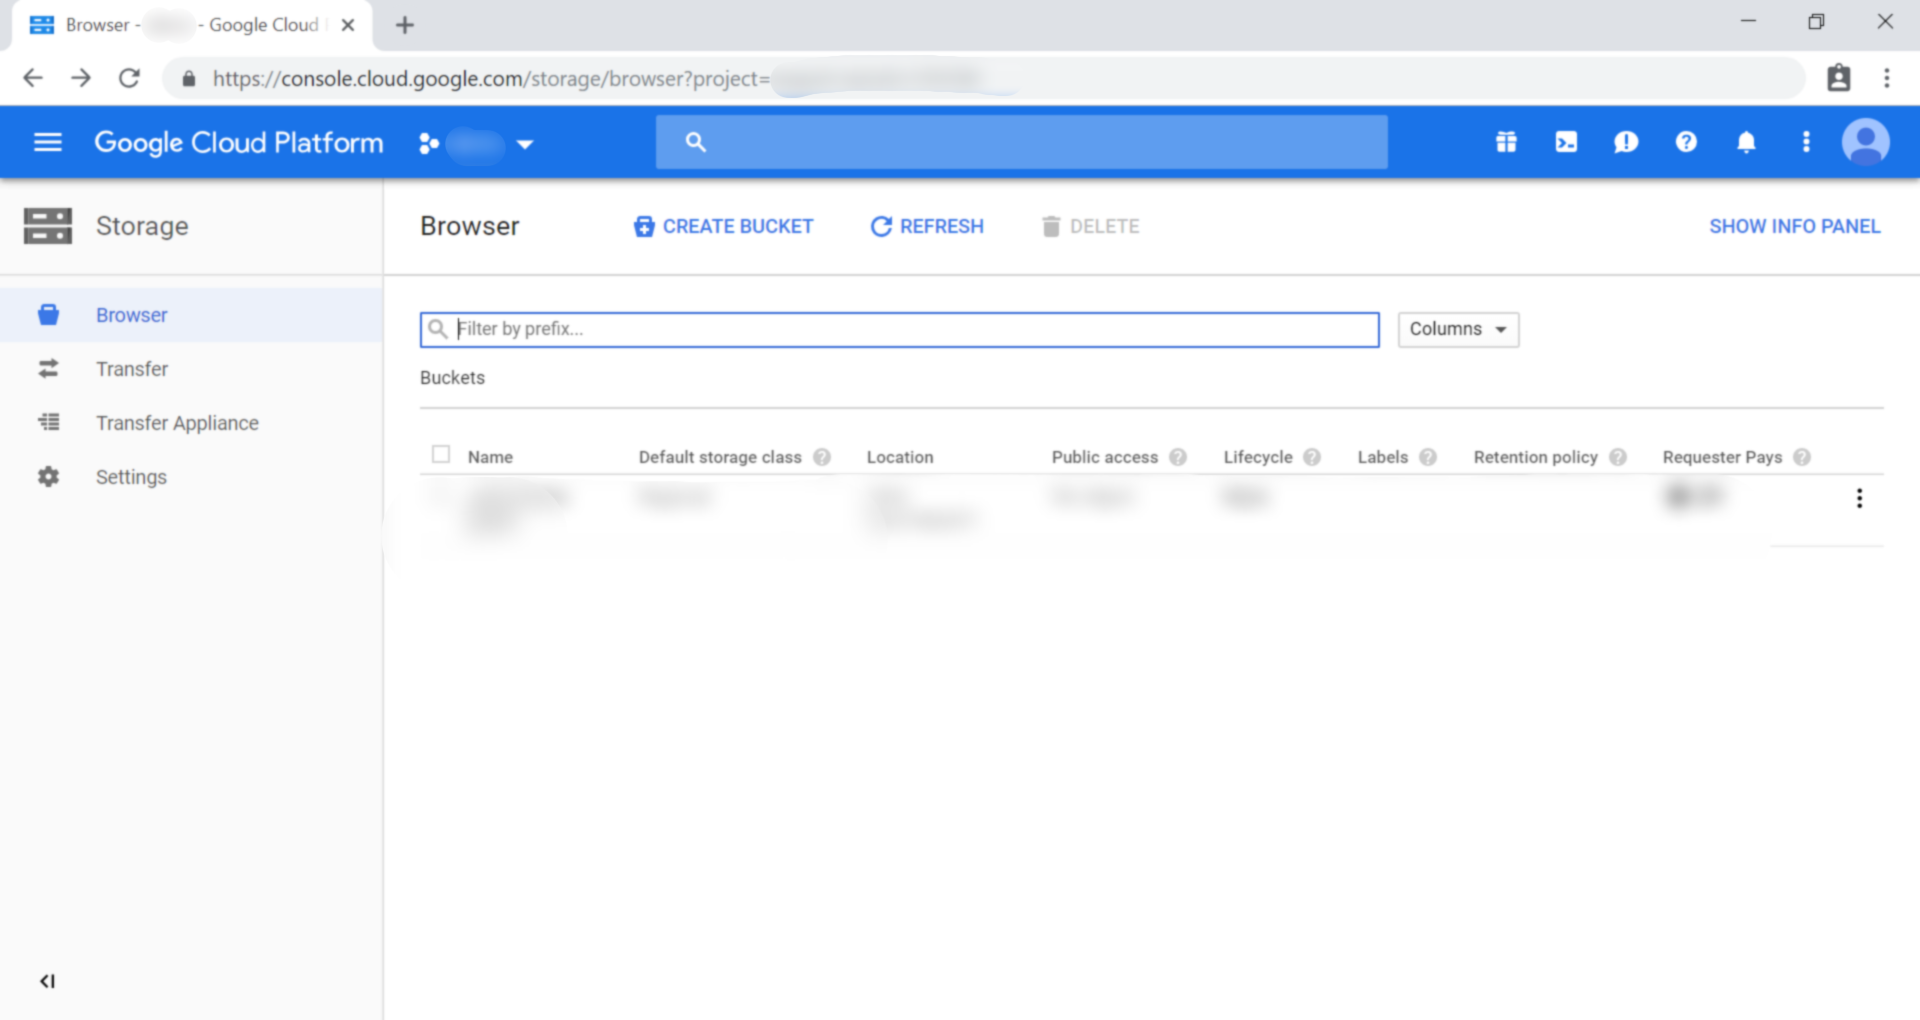
\includegraphics[width=0.6\columnwidth]{images/appendixA/GCP-Storage.PNG}
	      		\footcaption{Google Cloud Storage Management}
	      	\end{figure}
	      	\begin{figure}[H]
	      		\centering
	      		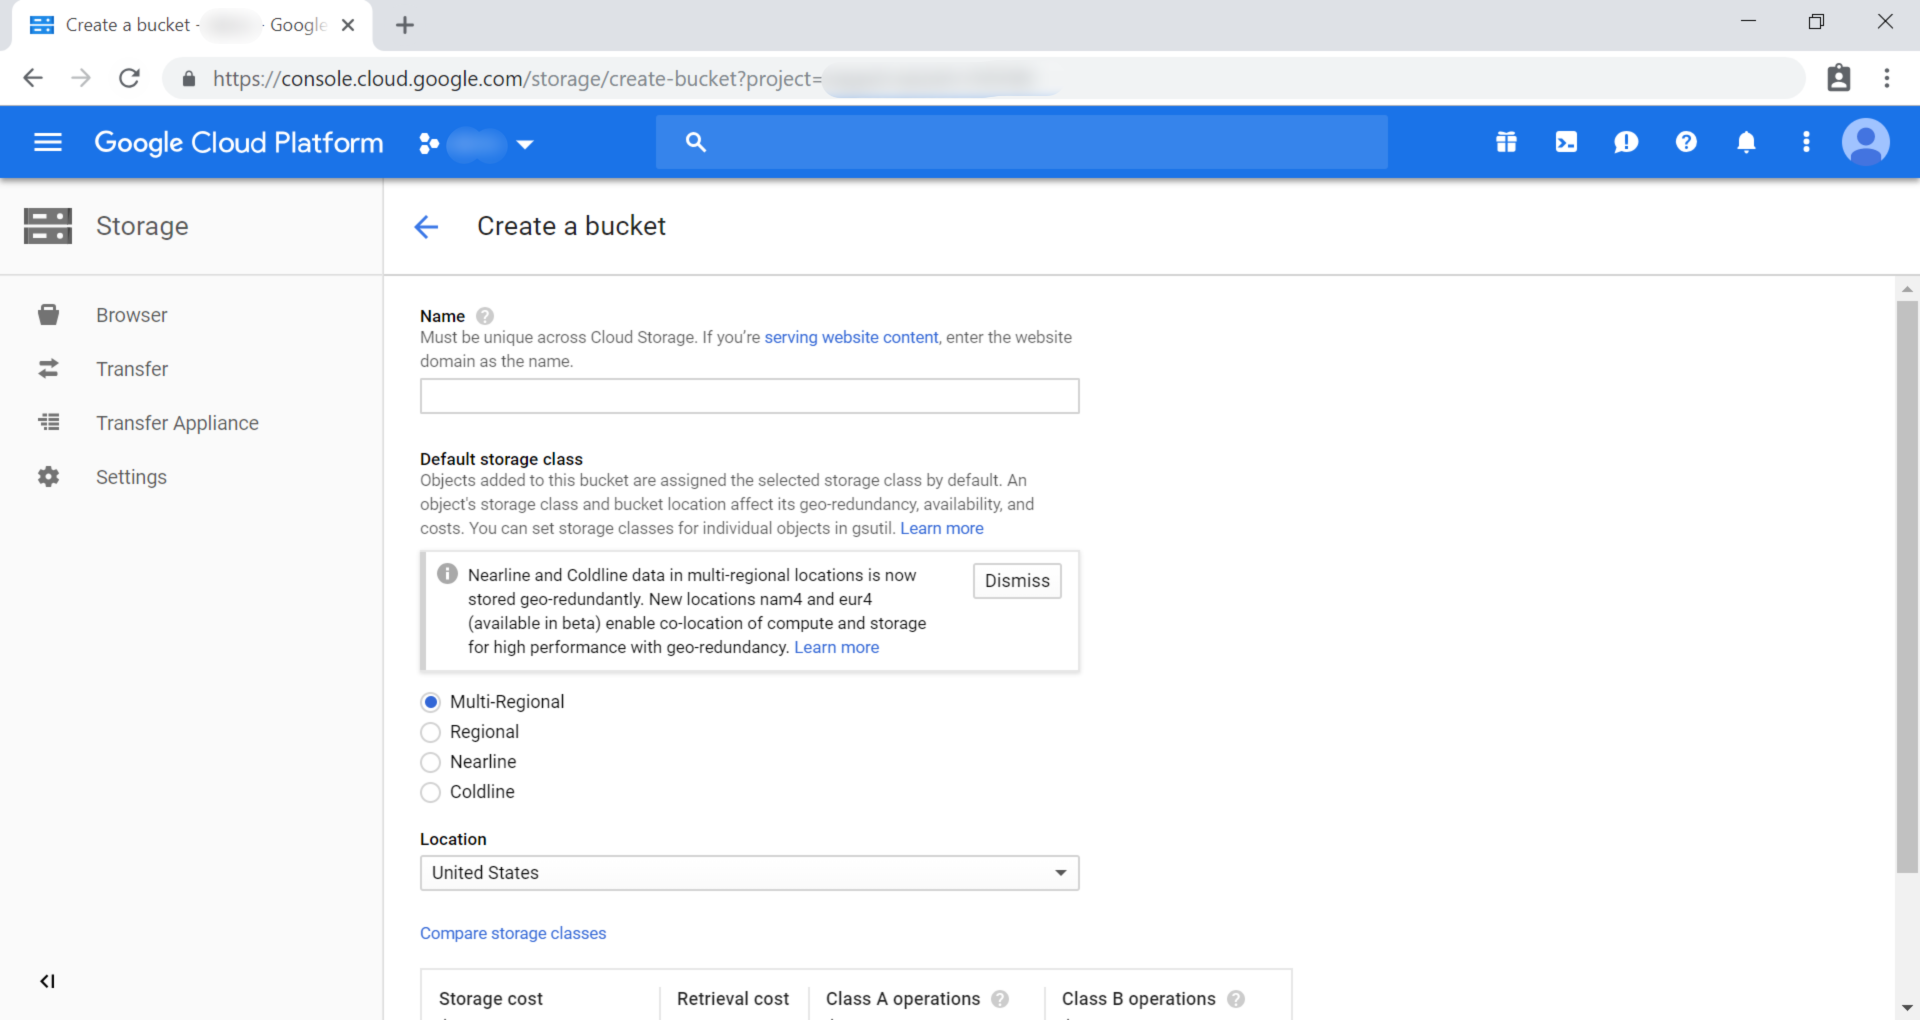
\includegraphics[width=0.6\columnwidth]{images/appendixA/GCP-Storage-create-bucket.PNG}
	      		\footcaption{Google Cloud Storage: Create Bucket}
	      	\end{figure}
	      \end{center}
	      \footnotetext{Source: \url{https://cloud.google.com/}}
	\item Following instruction in \href{https://cloud.google.com/iam/docs/creating-managing-service-accounts#creating_a_service_account}{https://cloud.google.com/iam/docs/creating-managing-service-accounts\#creating\_a\_service\_account} to create a \textit{Service Account} 
	\item Following instruction in \href{https://cloud.google.com/iam/docs/granting-roles-to-service-accounts#granting_access_to_a_service_account_for_a_resource}{https://cloud.google.com/iam/docs/granting-roles-to-service-accounts\#granting\_access\_to\_a\_service\_account\_for\_a\_resource} to grant role \textit{Storage Admin} for created \textit{Service Account}
	\item Following instruction in \href{https://cloud.google.com/iam/docs/creating-managing-service-account-keys#creating_service_account_keys}{https://cloud.google.com/iam/docs/creating-managing-service-account-keys\#creating\_service\_account\_keys} to create a \textit{Service Account key}. Download and keep it locally.
\end{enumerate}

\tocless\subsection{mLab}
\begin{enumerate}
\item Access \href{https://mlab.com/signup/}{https://mlab.com/signup/} and sign up an account
\item Click \textit{Create new} to create a new deployment
\item Click \textit{Users} and select \textit{Add database user}
\end{enumerate}

\tocless\subsection{Microsoft Cognitive Services}
\begin{enumerate}
\item Access \href{https://azure.microsoft.com/en-us/free}{https://azure.microsoft.com/en-us/free} and create an Azure account. For more detail, please follow this instruction \href{https://docs.microsoft.com/en-us/azure/cognitive-services/cognitive-services-apis-create-account}{https://docs.microsoft.com/en-us/azure/cognitive-services/cognitive-services-apis-create-account}
\item Create and subscribe to  Azure Cognitive Services: Face
\item Grab API keys
\end{enumerate}

\tocless\subsection{Facebook Account Kit}
\begin{enumerate}
\item Follow this documentation from \href{https://developers.facebook.com/docs/accountkit/webjs}{https://developers.facebook.com/docs/accountkit/webjs} to integrate Facebook Account Kit for Web. A Facebook Developer account is required.
\item After successfully integrated, Account Kit will appear below application name.
\item Access Account Kit Settings in application dashboard for more advanced configuration
\end{enumerate}

\tocless\subsection{SendGrid}
\begin{enumerate}
\item Access SendGrid’s homepage at \href{https://sendgrid.com/}{https://sendgrid.com/} and sign up an account
\item Get a SendGrid API key from \href{https://app.sendgrid.com/settings/api_keys}{https://app.sendgrid.com/settings/api\_keys}
\item Follow the instruction from The Official SendGrid Led, Community Driven Node.js API Library: \href{https://github.com/sendgrid/sendgrid-nodejs}{https://github.com/sendgrid/sendgrid-nodejs}
\end{enumerate}

\tocless\subsection{Google Maps API: Places Library}
\begin{enumerate}
\item Follow this tutorial (\href{https://developers.google.com/maps/documentation/javascript/tutorial}{https://developers.google.com/maps/documentation/javascript/tutorial}) to integrate Google Maps JavaScript API
\item Get a Google Maps API key from \href{https://developers.google.com/maps/documentation/javascript/get-api-key}{https://developers.google.com/maps/documentation/javascript/get-api-key}
\item Access \href{https://developers.google.com/maps/documentation/javascript/places}{https://developers.google.com/maps/documentation/javascript/places} for more detail about Places Library
\end{enumerate}

\tocless\subsection{Google OAuth 2.0 Authentication}
\begin{enumerate}
\item Follow this documentation (\href{http://www.passportjs.org/docs/google#oauth-2-0}{http://www.passportjs.org/docs/google\#oauth-2-0}) to integrate Google OAuth 2.0 Authentication
\item Follow this guide (\href{https://developers.google.com/adwords/api/docs/guides/authentication#webapp}{https://developers.google.com/adwords/api/docs/guides/authentication\#webapp}) to create a client ID and client secret for Google OAuth 2.0 Authentication
\item Go to Google API Console (\href{https://console.cloud.google.com/apis/dashboard}{https://console.cloud.google.com/apis/dashboard}) to manage Credentials (\href{https://console.cloud.google.com/apis/credentials}{https://console.cloud.google.com/apis/credentials}). For advanced configuration, select the just created OAuth 2.0 client ID
\end{enumerate}
\section{Source code}
\chapter{User manual}
\section{Verifying account}
1. Login with your account or register new account. 
\begin{center}
    \begin{figure}[H]
    \centering
    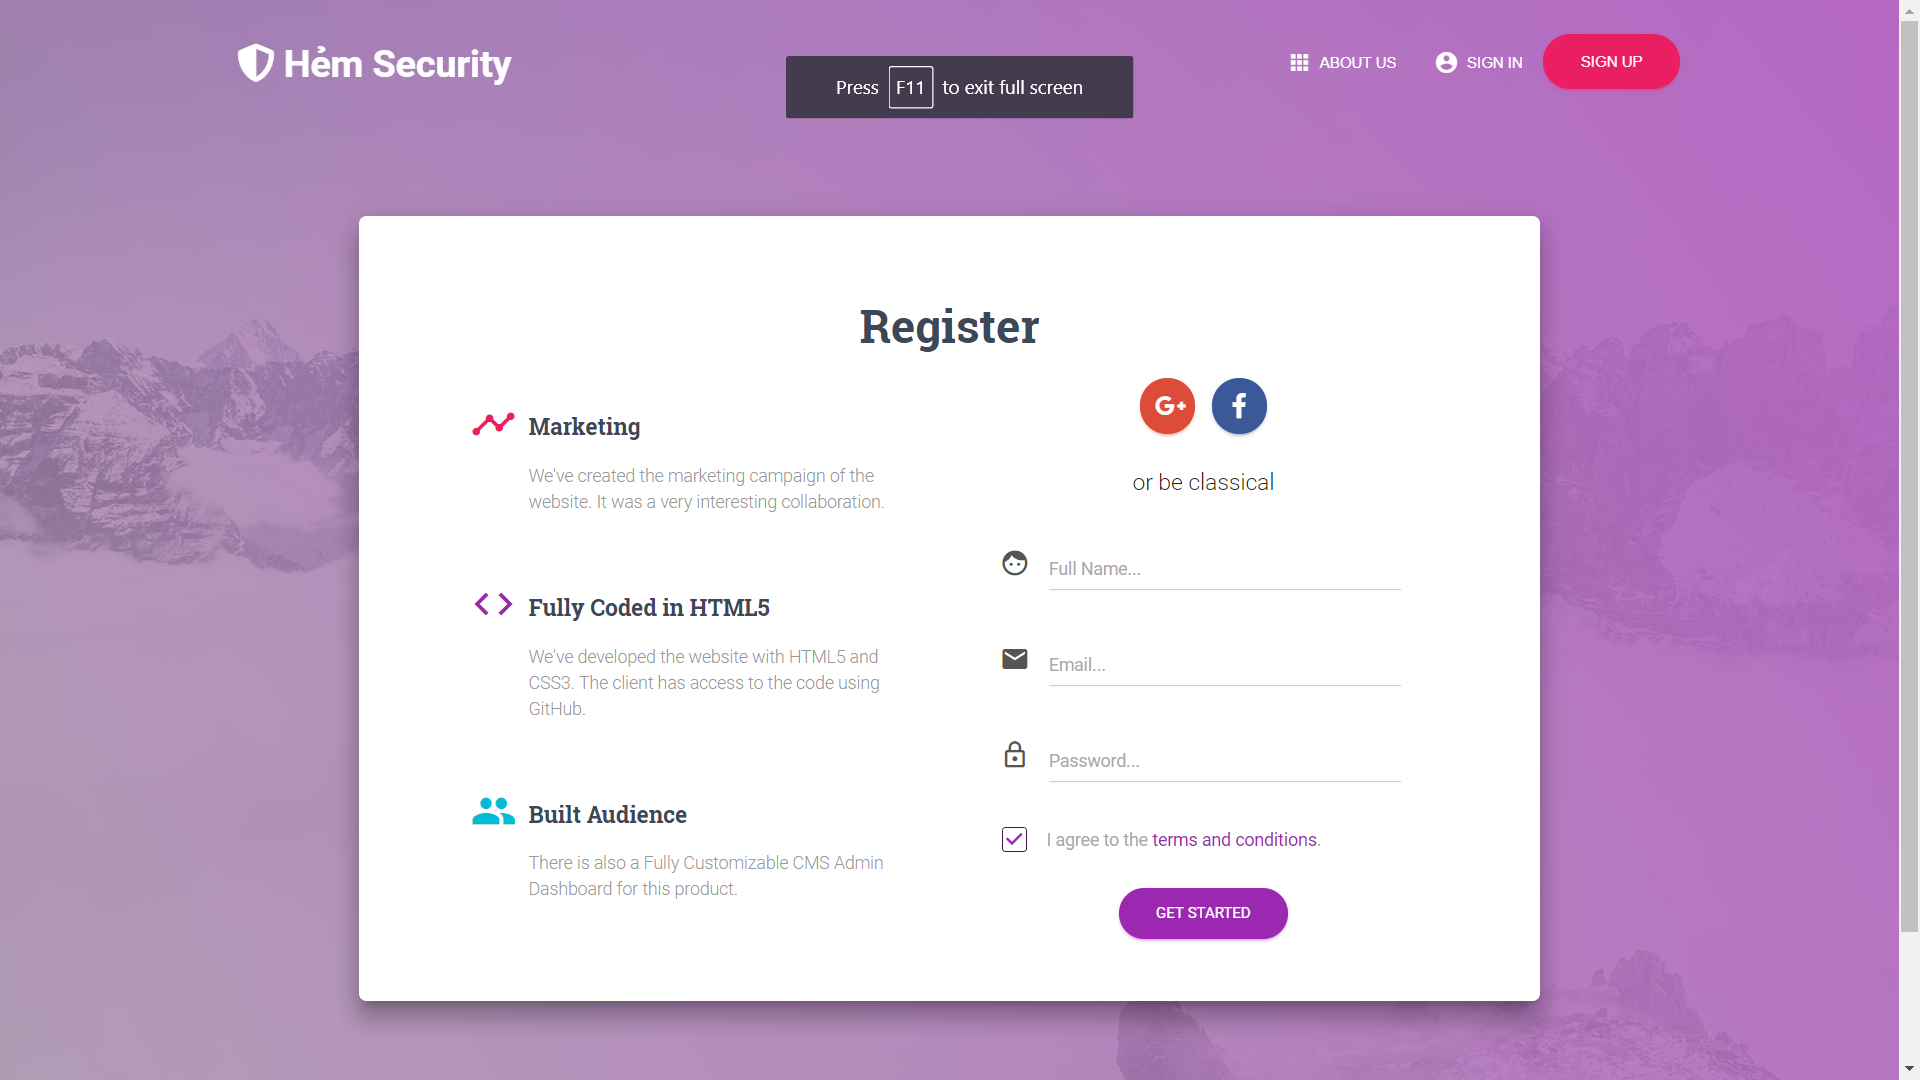
\includegraphics[width=1\columnwidth]{images/chap6/instruction1.png}
    \footcaption{Homepage}
    \label{}
    \end{figure}
\end{center}
2. Unverified account is unable to use most of the features, verify your account by clicking your name to go to your profile page
\begin{center}
    \begin{figure}[H]
    \centering
    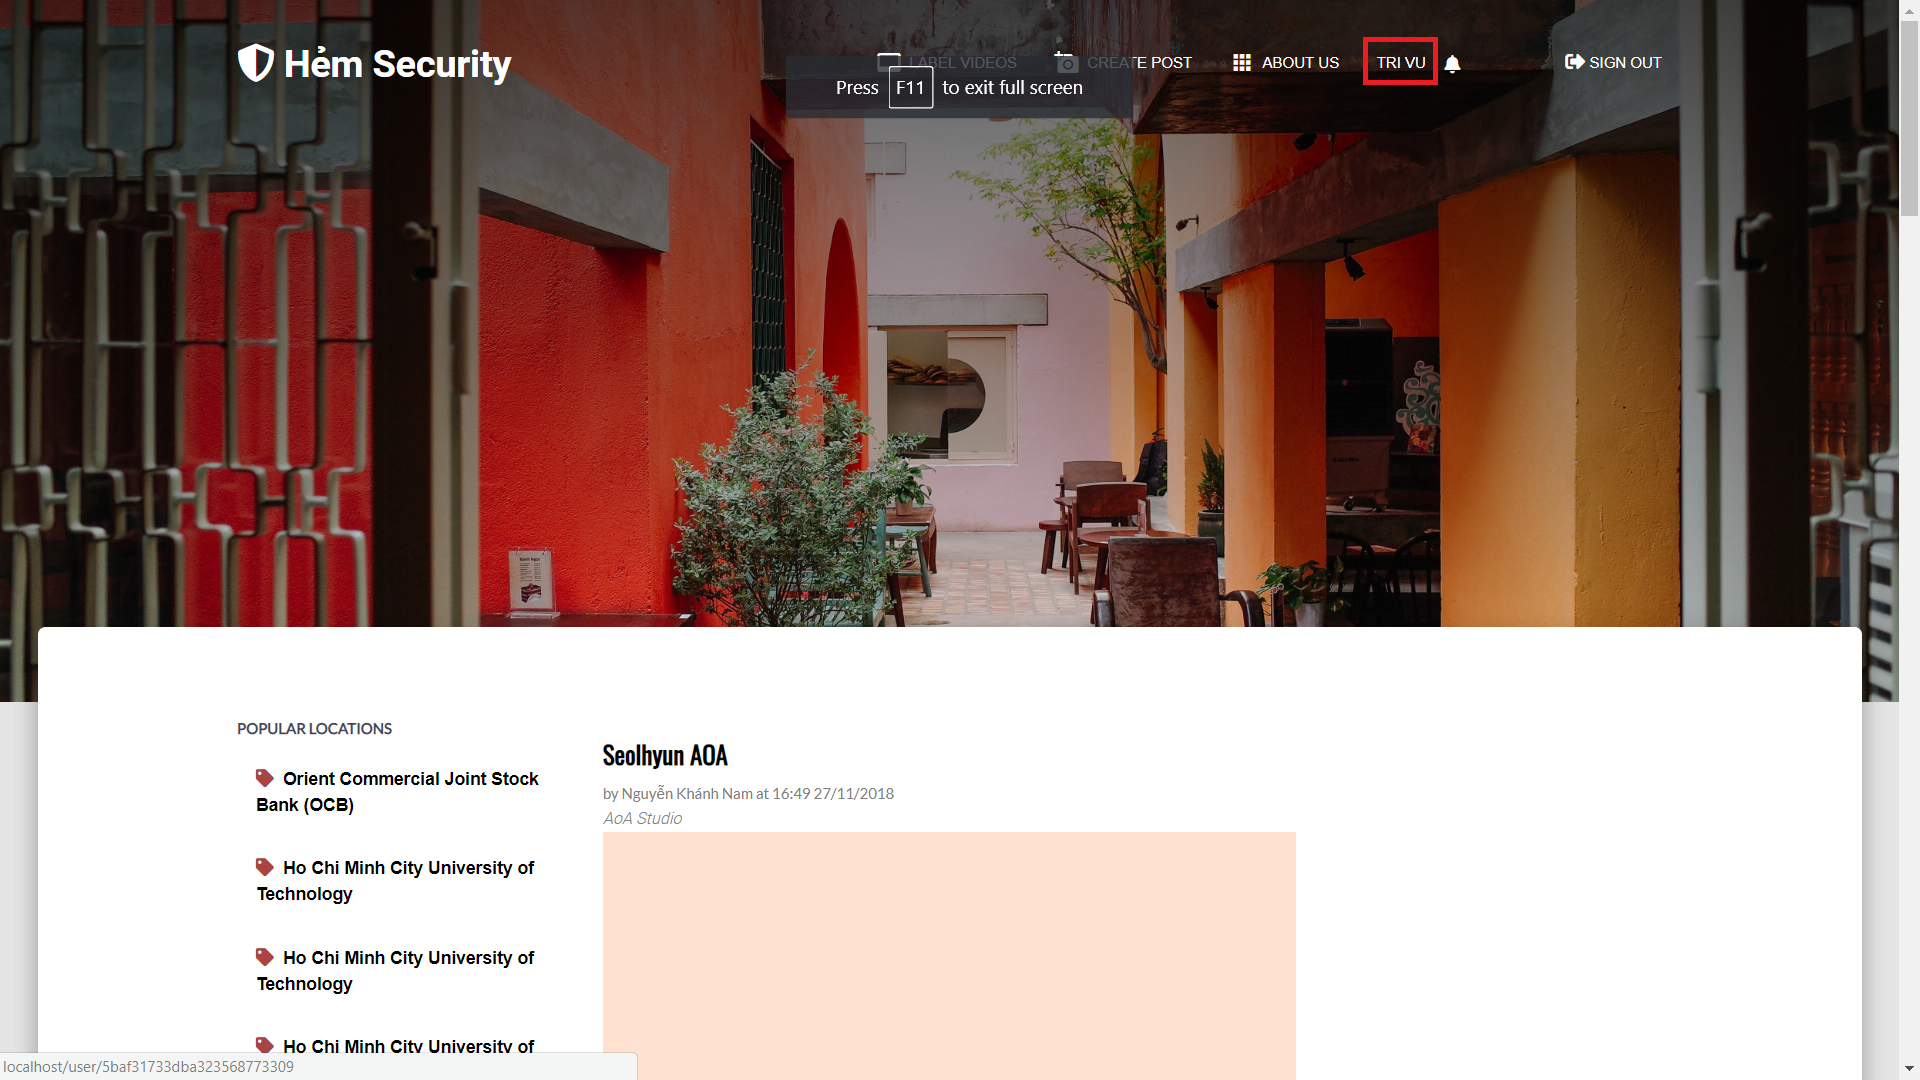
\includegraphics[width=1\columnwidth]{images/chap6/instruction2.png}
    \end{figure}
\end{center}
3. Enter your phone number to verify
\begin{center}
    \begin{figure}[H]
    \centering
    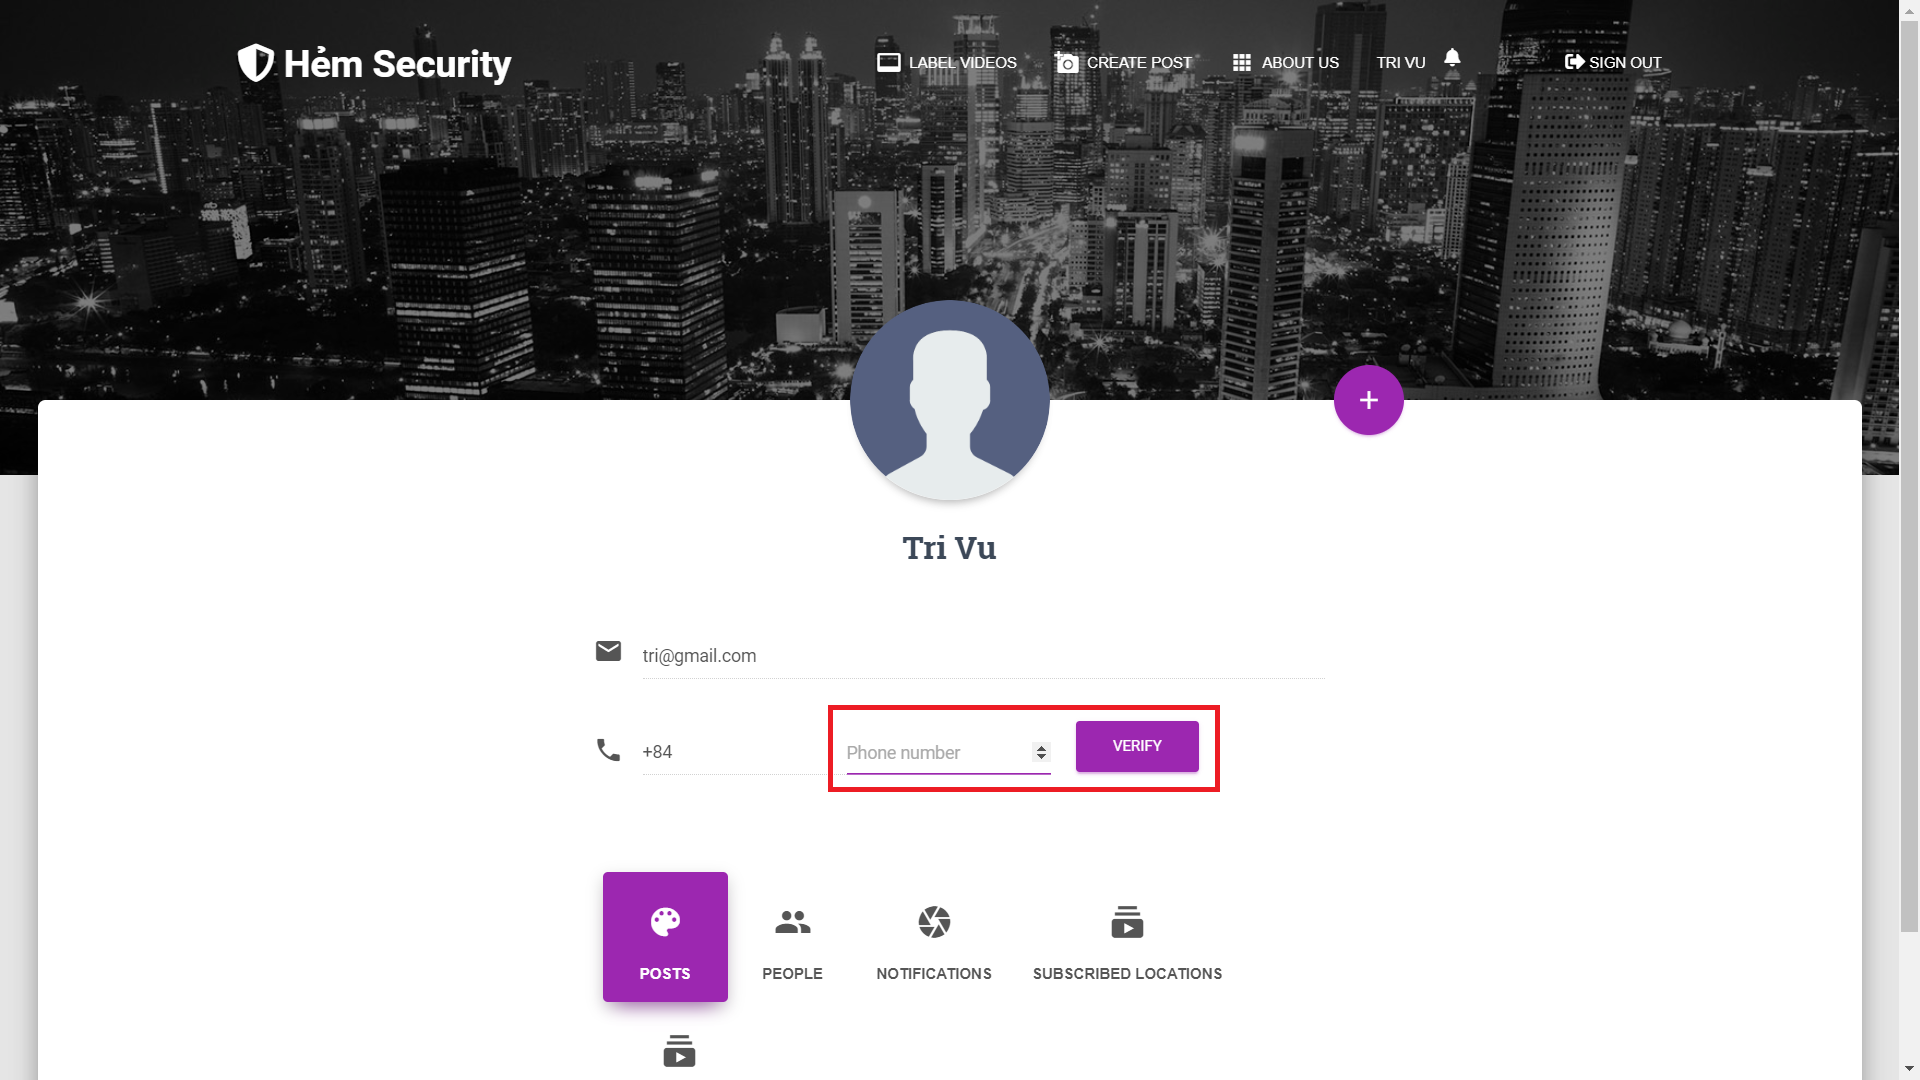
\includegraphics[width=1\columnwidth]{images/chap6/instruction3.png}
    \end{figure}
\end{center}
4. User can choose either to receive confirmation code by WhatsApp or SMS. Enter your code to finish verifying.
\begin{center}
    \begin{figure}[H]
    \centering
    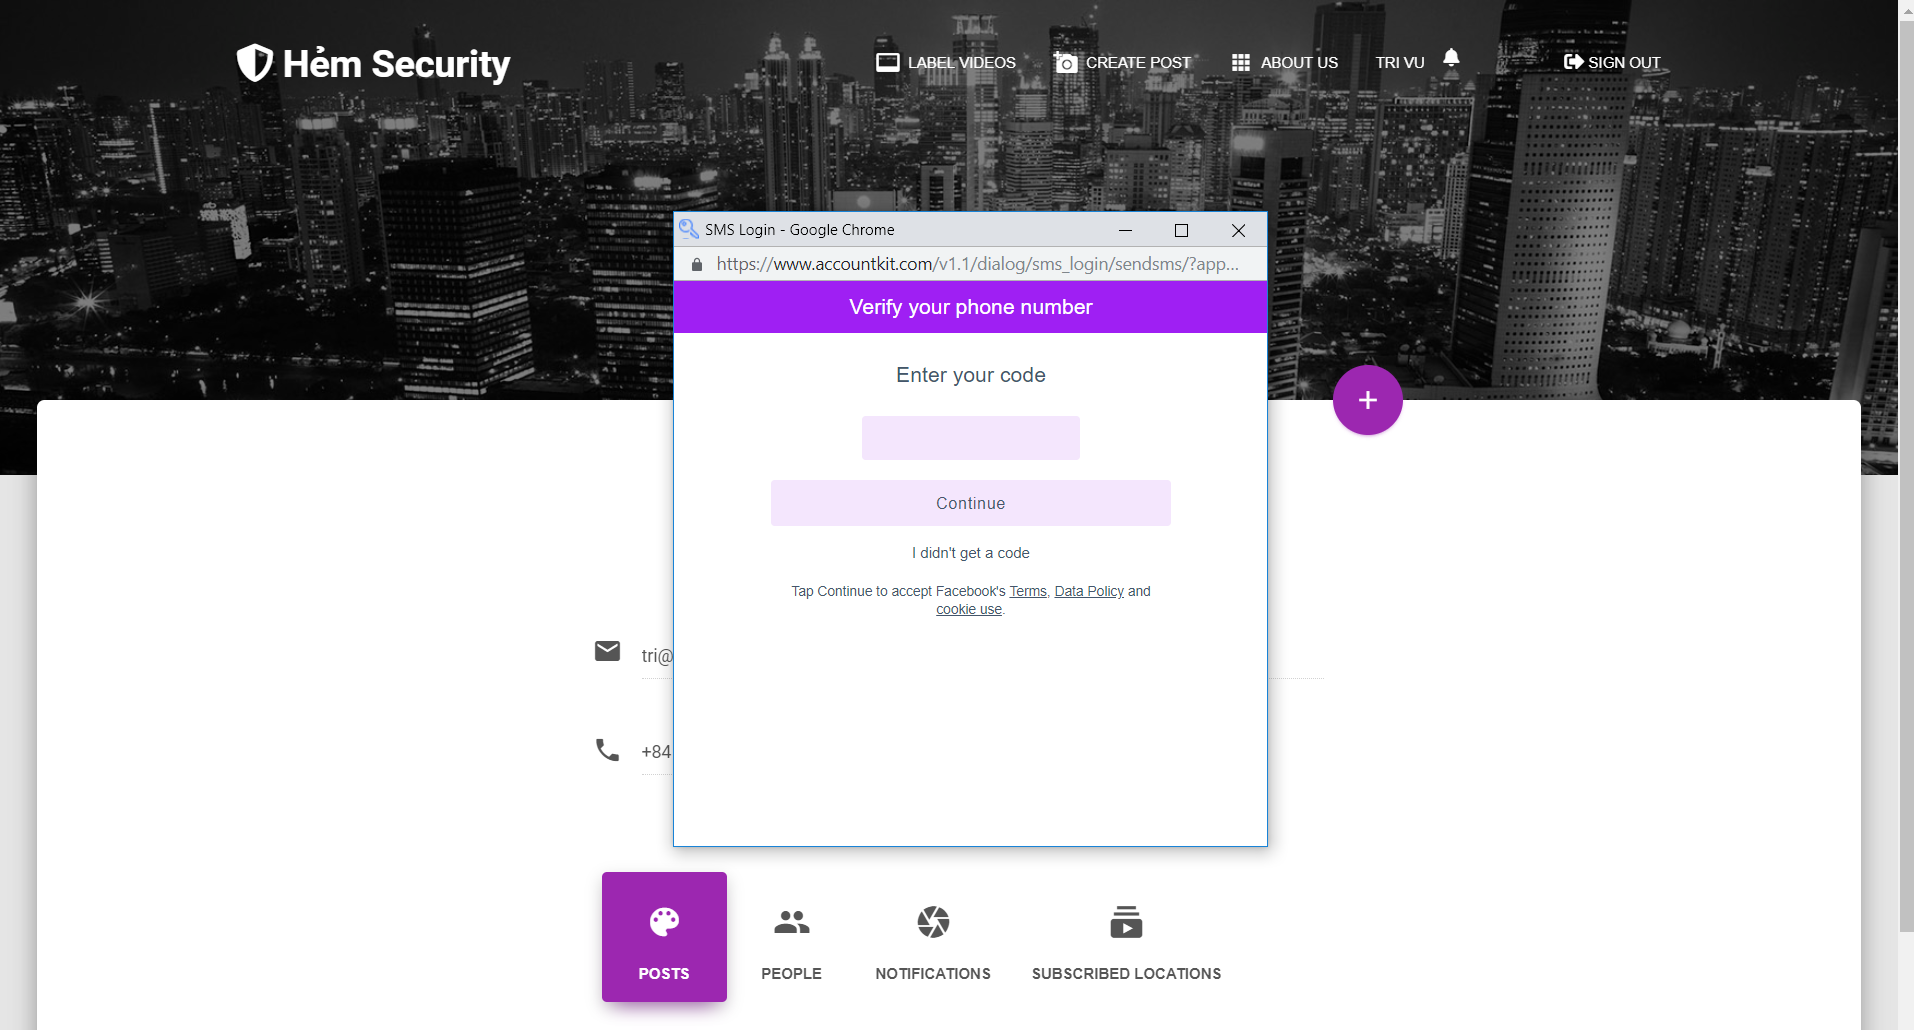
\includegraphics[width=1\columnwidth]{images/chap6/instruction4.png}
    \end{figure}
\end{center}
\section{Label video}
1. Go to "Label video" page
\begin{center}
    \begin{figure}[H]
    \centering
    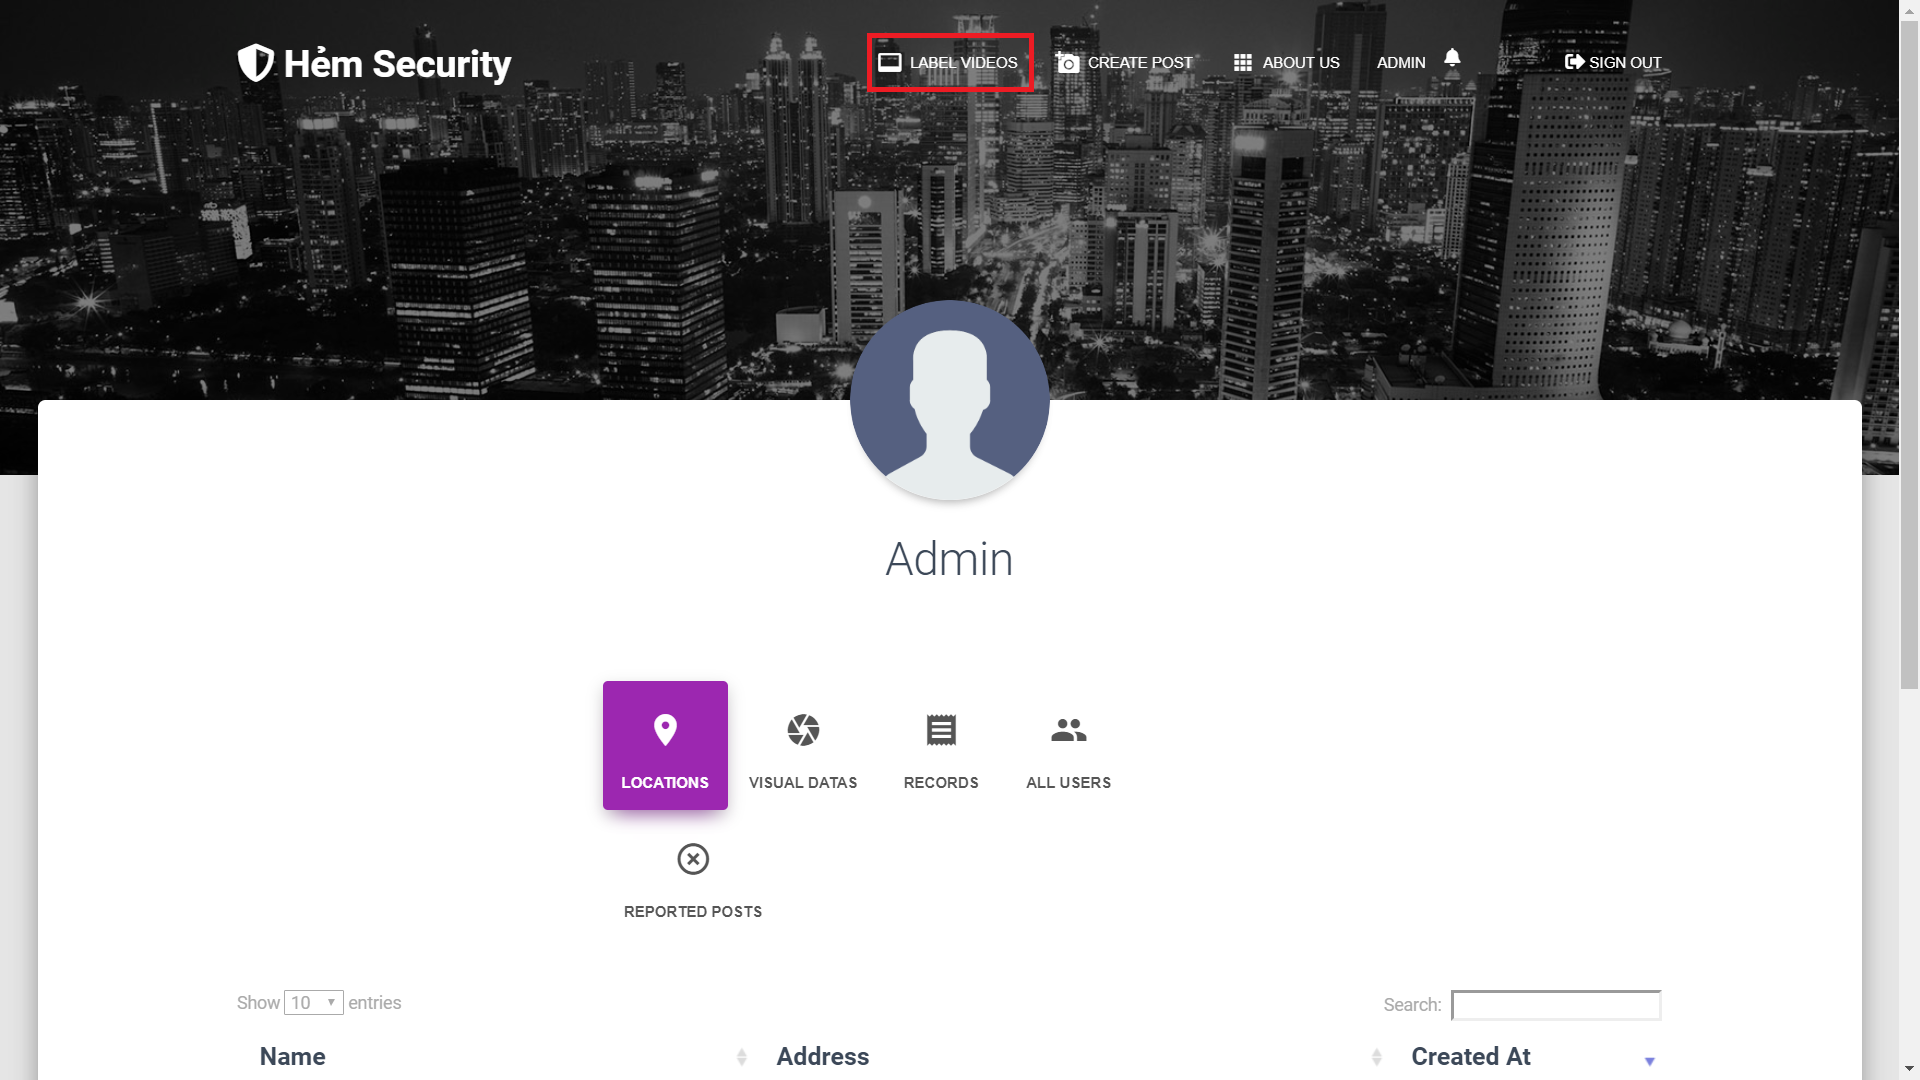
\includegraphics[width=1\columnwidth]{images/chap6/instruction5.png}
    \end{figure}
\end{center}
2. Choose either "Suspicious" or "Not suspicious". 
\begin{center}
    \begin{figure}[H]
    \centering
    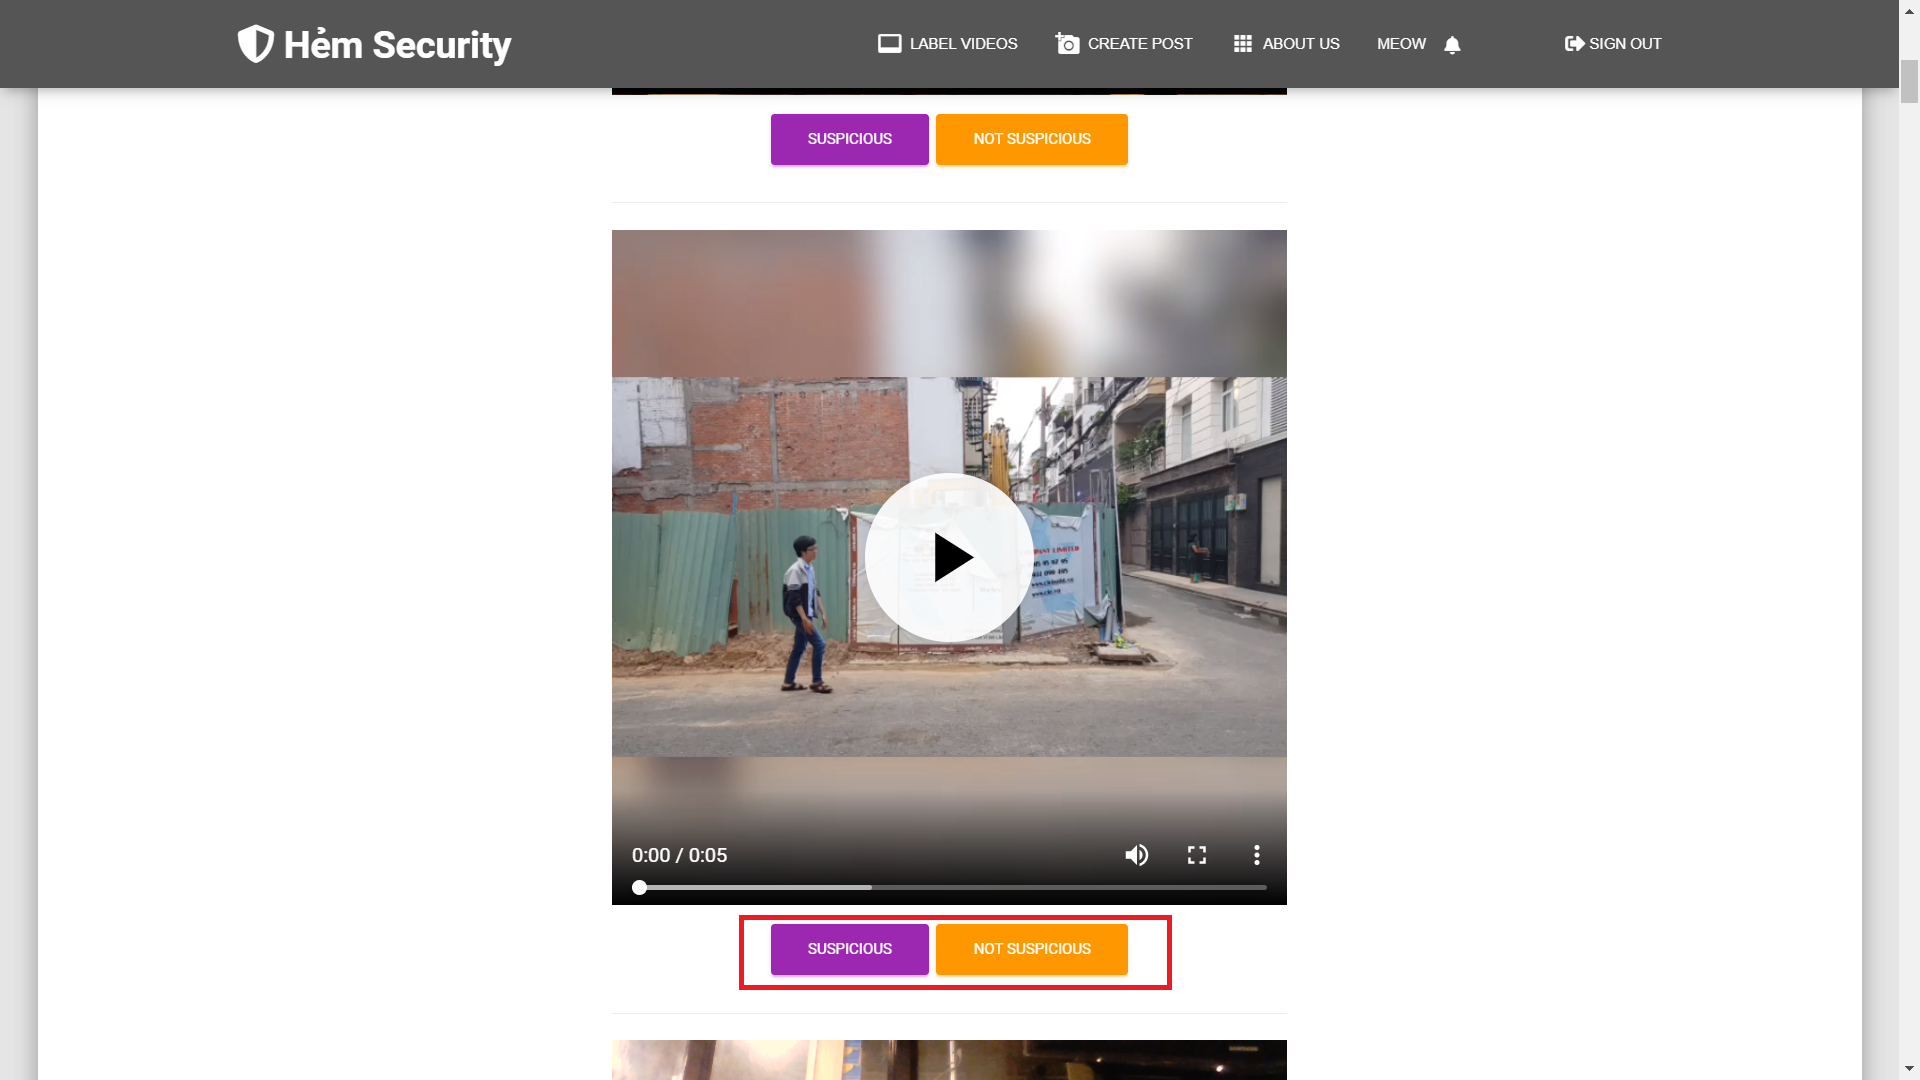
\includegraphics[width=1\columnwidth]{images/chap6/instruction6.png}
    \end{figure}
\end{center}
\section{Create post}
1. Go to "Create post" page
\begin{center}
    \begin{figure}[H]
    \centering
    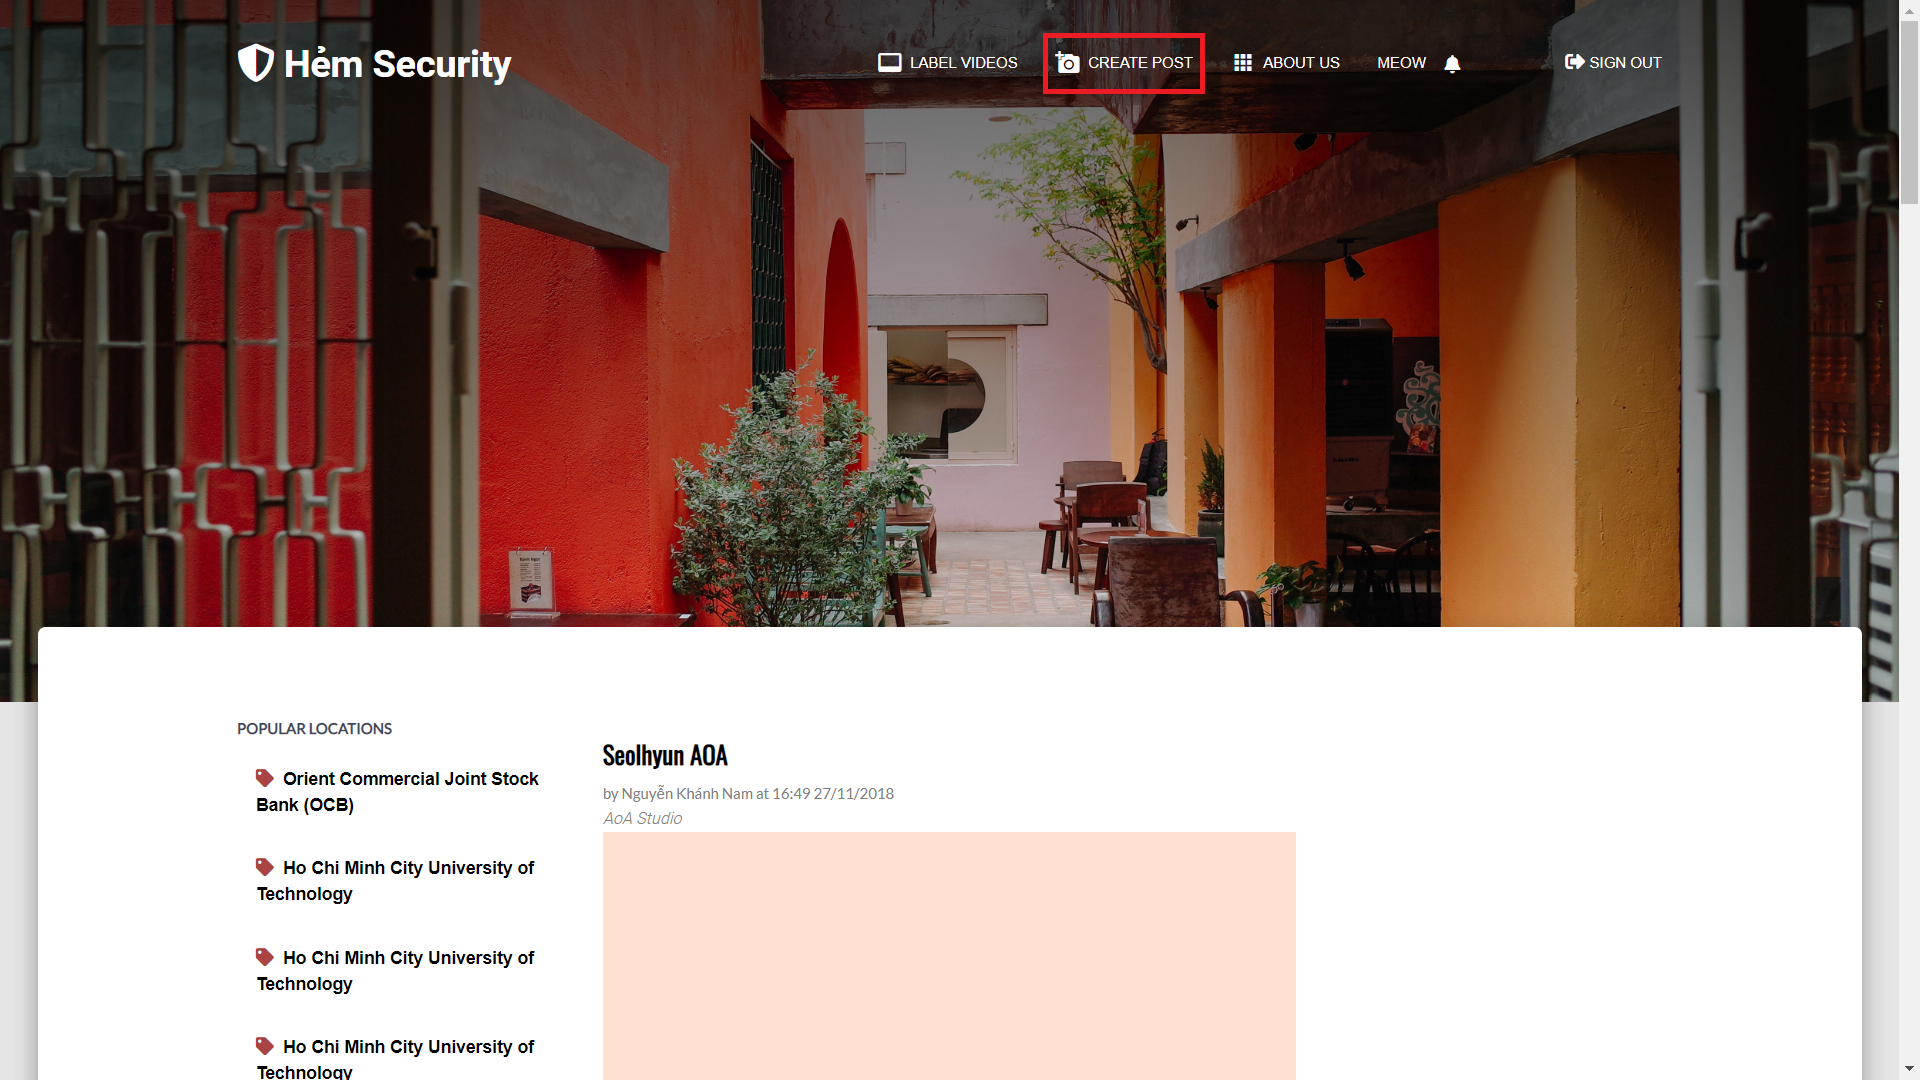
\includegraphics[width=1\columnwidth]{images/chap6/instruction7.png}
    \end{figure}
\end{center}
2. Fill in the form to and click "Create". 
\begin{center}
    \begin{figure}[H]
    \centering
    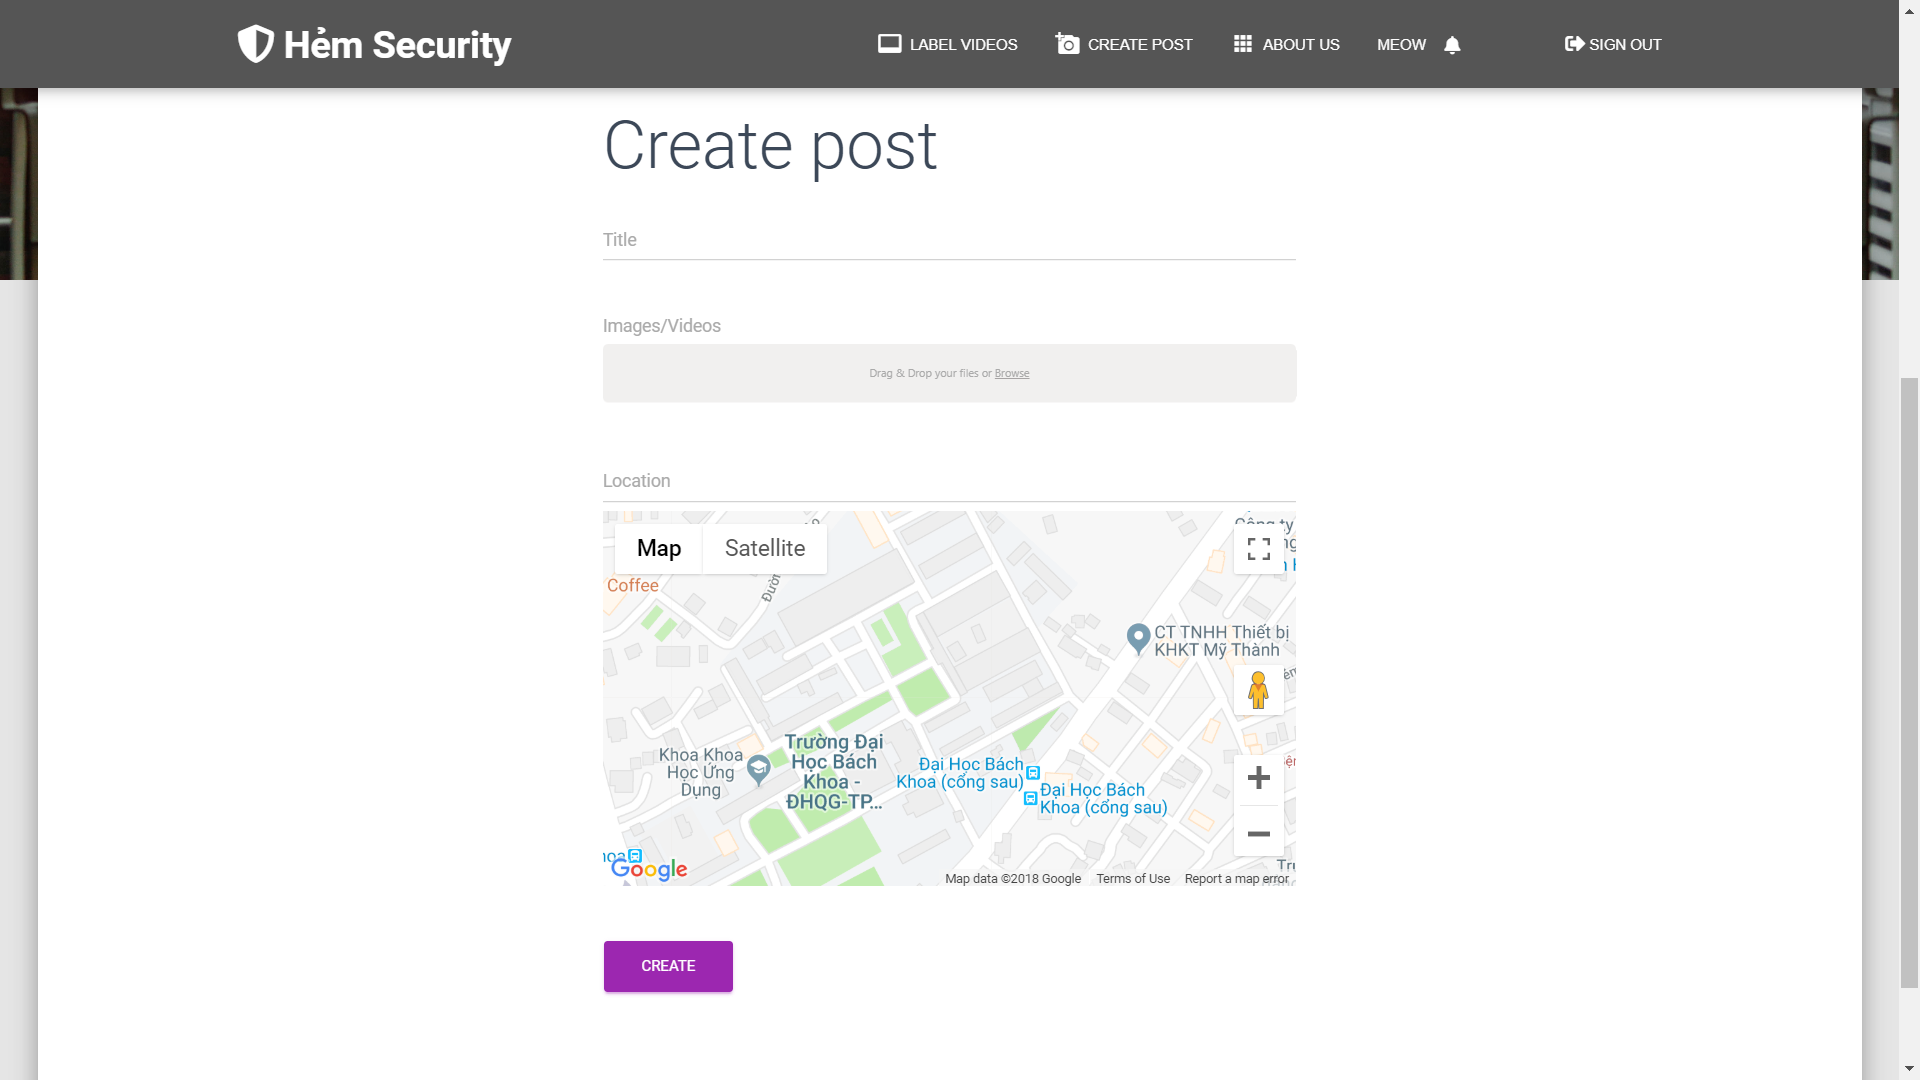
\includegraphics[width=1\columnwidth]{images/chap6/instruction8.png}
    \footcaption{Create post form}
    \end{figure}
\end{center}
\section{Subscribe a location}
1. Go to profile page and choose "All locations" tab
\begin{center}
    \begin{figure}[H]
    \centering
    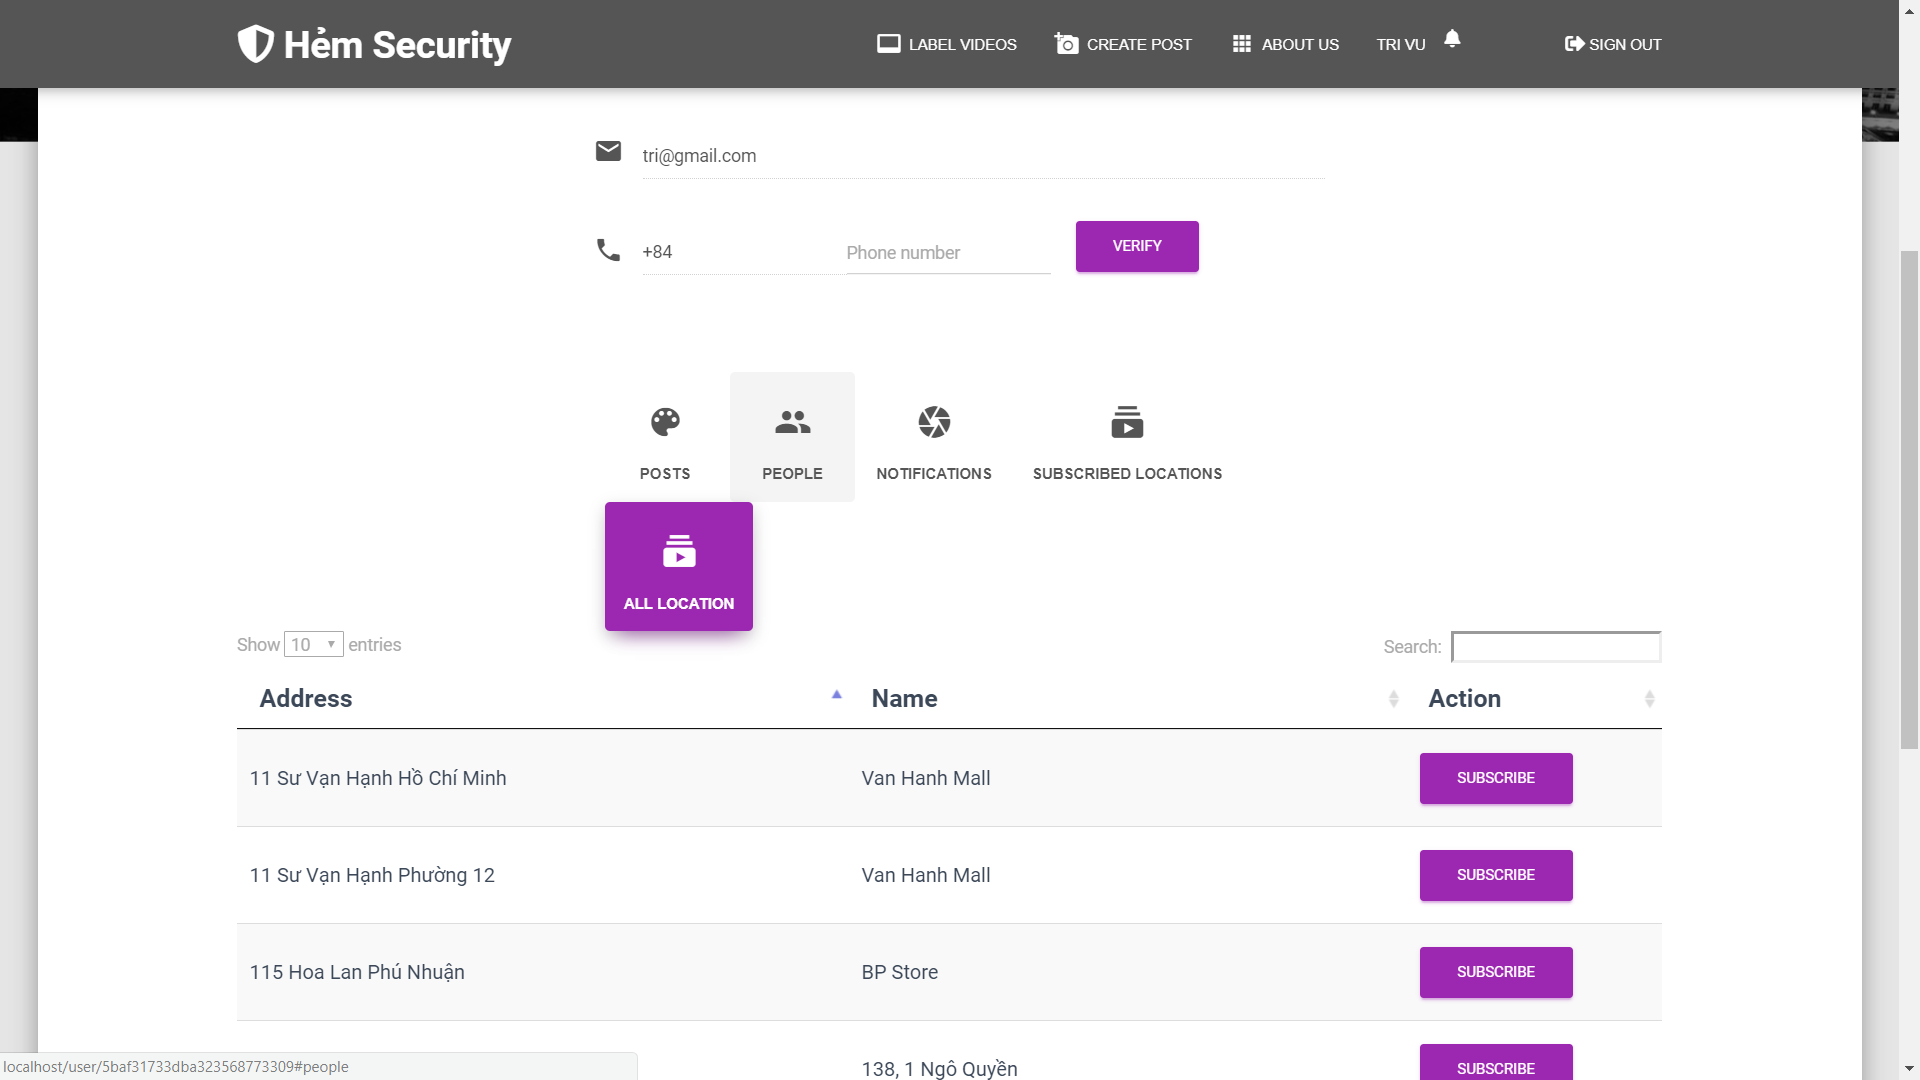
\includegraphics[width=1\columnwidth]{images/chap6/instruction9.png}
    \end{figure}
\end{center}
2. Choose a location to subscribe from the list. User will receive notification about suspicious behavior around subscribed location within a radius of 1 kilometer.   
\begin{center}
    \begin{figure}[H]
    \centering
    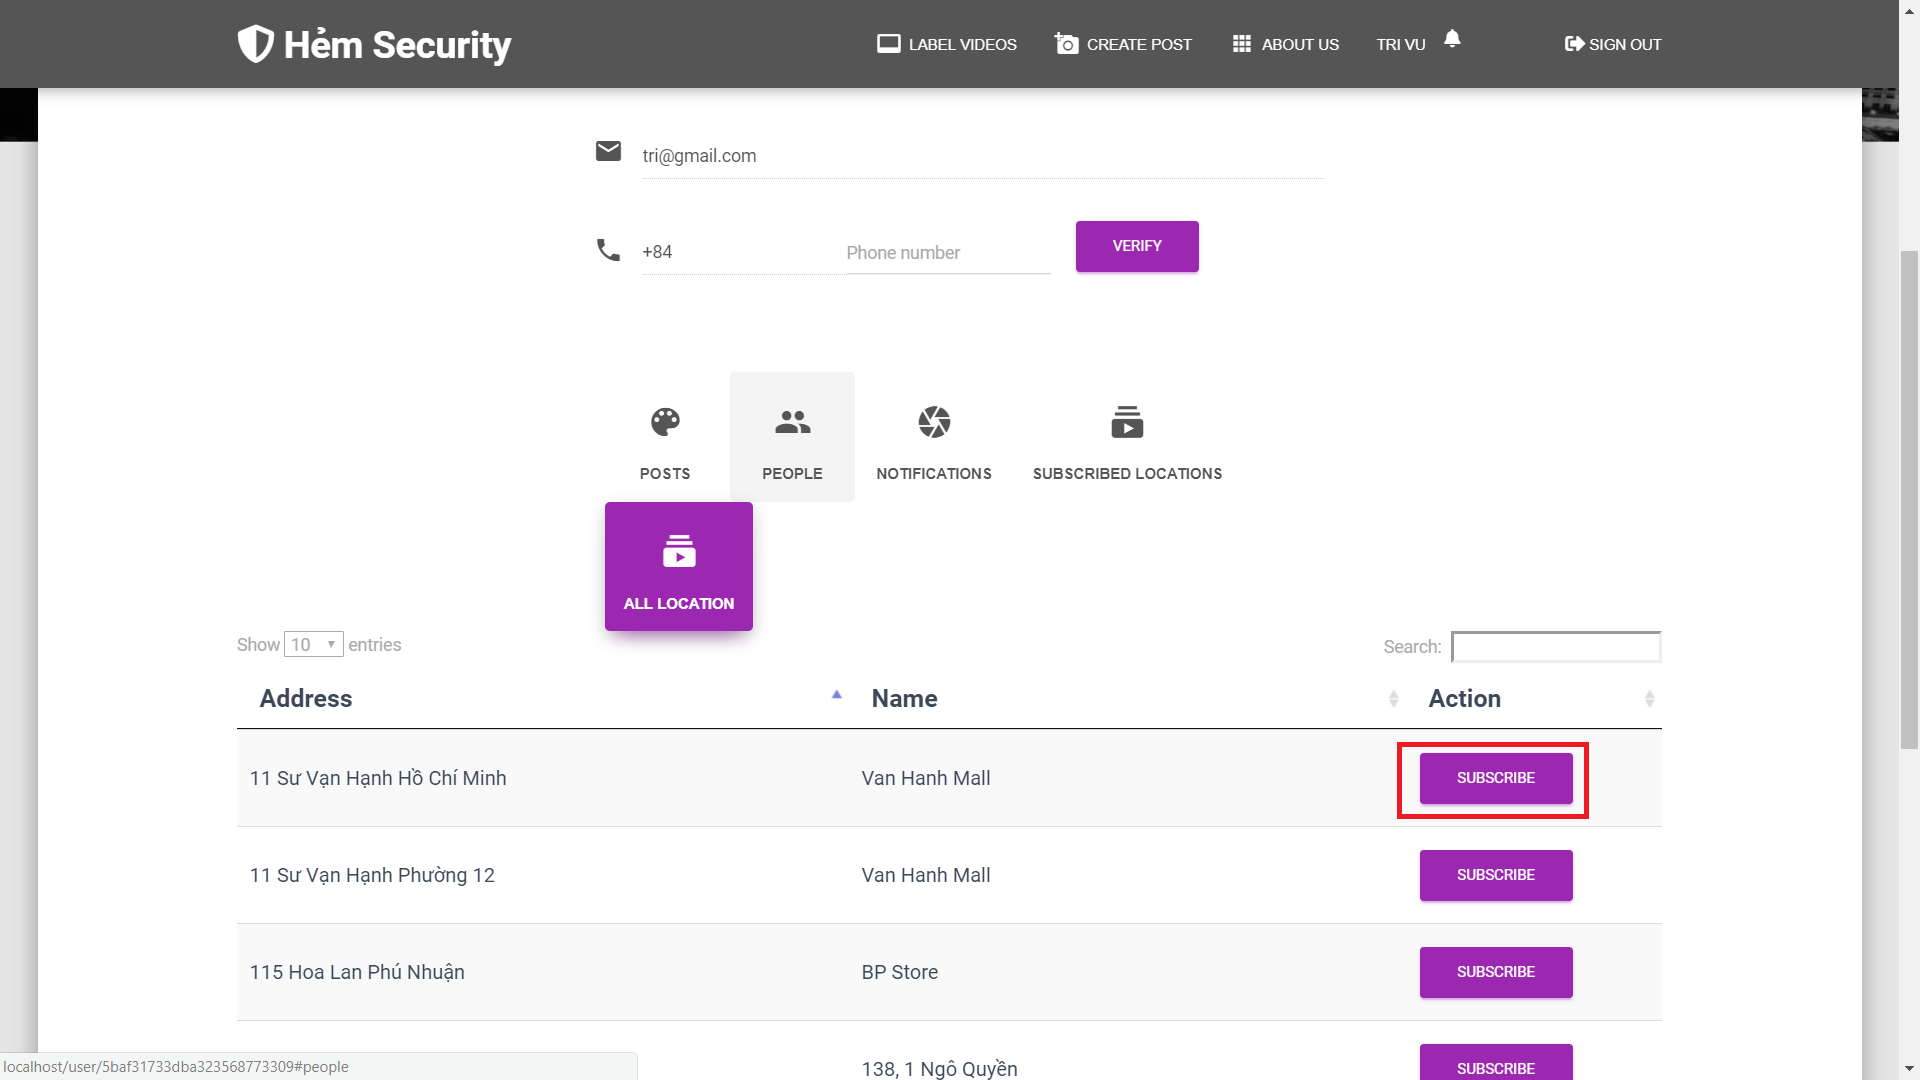
\includegraphics[width=1\columnwidth]{images/chap6/instruction10.png}
    \end{figure}
\end{center}



\cleardoublepage

% \renewcommand\bibname{TÀI LIỆU THAM KHẢO}
\bibliographystyle{ThesisStyle}
\bibliography{Thesis}

\cleardoublepage

\end{document}
%\appendix
%\chapter{The Soft Sensor -  BEO}
\label{chap:appendix1}

\section{Architecture of BEO}

\begin{figure}[H]
  \centering
  \includegraphics[width=1.0\textwidth]{images/Chap5/BEOArchitecture.pdf}
  \caption{Architecture of BEO}
  \label{App:fig01}    
\end{figure}

Figure \ref{App:fig01} shows our system architecture, namely BEO - Boiler Efficiency Optimization. The system includes several complex modules. We present these modules as follows.

\subsection{Real-Time Monitoring} 

This module is an OPC (OLE for Process Control) Client collecting automatically data from OPC Server via a local network. OPC is a software interface standard that allows Windows programs to communicate with industrial hardware devices\footnote{\url{http://www.opcdatahub.com/WhatIsOPC.html}}. In every duration, the tool gets parameter's values from OPC Server and the value of duration is defined by the user, usually 60s.

\subsection{Data Pre-Processing} 

The module has two main functions: (i) Reading raw operational data from several separate historical text files or receiving real-time data from the real-time monitoring module; then analyzing the data structure and storing the data into a unit database (SQL Server DBMS); (ii) Cleaning the database to make sure it has no errors, outliers, and noisy data. Each record in the database consists of control parameters, load of the boiler, and a corresponding boiler efficiency.

\subsection{Data Clustering} 

Since the system works in real-time, the operational data is enormous. Reducing the size of the operational data is significant in speeding up the system to meet its real-time requirement. Data clustering is to group similar records into the same cluster, and derives a knowledge base consisting of the centers of those clusters. 

\subsection{Anomaly Detection}

This module is responsible for detecting anomalies of the real boiler during operating. The module is integrated in Pre-Processing data Module to remove outliers. Moreover, the module detects some abnormalities caused by unknown reasons and warns the operators to determine timerly solutions.  

\subsection{Efficiency Calculator}

The boiler efficiency can be calculated by the boiler simulator module. Typically, boiler simulator only works on M important parameters that are chosen by experts. However, each tuple of the operating data is a set of N parameters and N is usually larger than M. Several formulas can calculate the boiler efficiency from full N parameters. Unfortunately, these formulas are very complex. Two methods are used in the BEO soft sensor to calculate the boiler efficiency \cite{boi:ref_11}.

\begin{itemize}

\item \textit{Direct Method:} The boiler efficiency is the ratio of the energy obtained from steam and the energy of the fuel in the boiler.
\item \textit{Indirect Method} The boiler efficiency is the difference between energy loss and energy input.

\end{itemize}

\subsection{Boiler Efficiency Simulation}

Combustion is considered as a process of time-oriented technology, and the equation of state combustion efficiency is a complex nonlinear equation where coefficients are not fixed. It is difficult to exactly find coefficients of that nonlinear equation. As a result, we need an approximate solution. Neural networks seem to be a simple and effective approximation scheme for this kind of problem. In BEO soft sensor, the boiler with the internal reaction equations is monitored as a black box with control parameters and an corresponding output called the boiler efficiency. Therefore, we need a boiler simulator for simulating the real boiler from the operational data. The boiler simulator determines the correlation between the control parameters and the boiler efficiency. The control parameters consisting of air flow, air pressure, water flow, etc. to operate the boiler. The boiler is simulated by a multi-variable equation $y = f(x_1, x_2, ..., x_n)$, where $x_i$ is a control parameter, $y$ is a boiler efficiency, and $f(.)$ is a suggested model, e.g., neural networks. This modeling of the boiler helps us to build a boiler simulation with technological features like a real boiler. Among many advanced techniques that can approximate the real boiler, such as fuzzy systems, support vector machines, etc., RFNN is chosen due to its straightforward idea and easy deployment.

As presented in detail in Section \ref{chap:boilerefficiencyoptimization}, the Boiler Efficiency Simulation Module is implemented by RFNN with mean absolute relative error (MARE) approximately $2.04E-03$ and $2.97E-03$, in the training phase and the testing phase, respectively.

\subsection{Boiler Efficiency Optimization}

At the time of the boiler efficiency appears downtrends, this module detects in knowledge base and finds a tuple of control parameters that gives higher efficiency than current efficiency. The controllable parameters will be changed by the new values in the found tuple. After suggesting the new parameter values, the Boiler Efficiency Simulation Module predicts the boiler efficiency according to these new values. In the case of the predicting efficiency is lower than the current efficiency; the suggestion will be ignored. Conversely, this module will apply the new found parameters for the boiler with expecting an improved boiler efficiency. Process working of the module is illustrated in Figure \ref{App:fig02}, and it has several steps as follows.

\begin{itemize}

\item \textit{Step 1:} Reading data from OPC Server via the Real-Tiem Monitoring Module.
\item \textit{Step 2:} Finding some similar tuples with the current control parameters that have higher efficiency than the current and have the same load.
\item \textit{Step 3:} Checking whether the change of load is higher than a delta value. That the change is not higher a delta value indicates the load is stable and the module can adjust parameters to improve boiler efficiency. Conversely, that the change is higher a delta value indicates the load is not stable, the module ignores and continue monitoring.
\item \textit{Step 4:} In the case of stable load, if the new similar tuples can give higher efficiency that is predicted by the Boiler Efficiency Simulation Module, these tuples will be applied to improve the boiler efficiency.

\end{itemize}

\begin{figure}[H]
  \centering
  \includegraphics[width=0.5\textwidth]{images/Appendix1/BoilerOptimization.pdf}
  \caption{Real-time optimization work-flow}
  \label{App:fig02}    
\end{figure}

\subsection{Boiler Controller}

The same as the Real-Time Monitoring Module, the Boiler Controller Module is an OPC Client controlling the real boiler through OPC Server. According to some adjustments recommended by the Real-Time Boiler Efficiency Optimization Module, the Boiler Controller Module adjusts the control parameters of the real boiler to improve its efficiency.

\subsection{Multi-Step-Ahead Real-Time Forecasting}

As presented in \ref{chap:boilerefficiencyoptimization}, this module is responsible for forecasting the downtrends of boiler efficiency. In the case of down-trend appearances, this module will inform to the Real-Time Boiler Efficiency Optimization Module to proceed the adjustment of control parameters.

\section{Benefit of BEO}

We employed a statistical method called statistical inference for two samples \cite{boi:ref_14} to assess the efficiency of the BEO soft sensor to Phu My Fertilizer Plant. Note that, to calculate confidently, this method requires that the size of samples must be large so that Student's t-distribution comes close to a normal distribution. We collected the operational data with the duration of 1 sample/60s. 

Data used for assessment was collected in 17 days with two separate periods: (i) 1st period: from November 02, 2013 to November 07, 2013, the size of samples is 5892 and the boiler load distributes from 76 ton/h to 83 ton/h. (ii) 2nd period: from November 08, 2013 to November 18, 2013, the size of samples is 8834 and boiler load distributes from 72 ton/h to 84 ton/h. We defined the minimum size of samples is 30 for each boiler load. During the time of collecting data, the boiler operation was in auto-mode and the boiler load is continuous. Therefore, we must rounded many values of boiler load to get one rounded value. For example, all boiler loads from 68.5 ton/h to 69.49 ton/h are rounded to 69 ton/h. After collecting data, we employed the statistical inference method to prove that the BEO soft sensor improve the performance of power consumption. 

As mentioned in \cite{boi:ref_14}, Student's t-distribution is one of normal distribution families. In Student's t-distribution, mean of $n$ observed data is estimated as below.

\begin{equation}
\bar{x} = \frac{\sum_{i=1}^nx_i}{n},
\end{equation}

and standard deviation $\sigma$:

\begin{equation}
\sigma = \sqrt{\frac{\sum_{i=1}^n(x - \bar{x})}{n-1}}.
\end{equation}

We define some factors that are used in Tables \ref{App:table02} and \ref{App:table03}.

\begin{itemize}
\item During running the boiler with BEO, the mean of power consumption is $\bar{x}^{BEO}$.
\item During running the boiler with BEO, the standard deviation of power consumption is $\sigma_{\bar{x}}^{BEO}$.
\item During running the boiler without BEO, the mean of power consumption is $\bar{x}^{noBEO}$.
\item During running the boiler without BEO, the standard deviation of power consumption is $\sigma_{\bar{x}}^{noBEO}$.
\end{itemize}

\begin{table}[H]
\scriptsize
  \begin{center}
    \begin{tabular}{c c c c c c c}
    \toprule
    \multirow{2}{*}{Load} & \multicolumn{2}{c}{With BEO} & \multicolumn{2}{c}{Without BEO} & \\[0.2cm]
    \cmidrule{2-7}
     & $\bar{x}^{BEO}$ & $\sigma_{\bar{x}}^{BEO}$ & $\bar{x}^{noBEO}$ & $\sigma_{\bar{x}}^{noBEO}$ & Confidence \% & Quantity of Improvement \%\\
    \midrule
	76 & 2.73603 & 0.00853 & 2.83275 & 0.00683 & 100.00 & 3.41\\
    77 & 2.73761 & 0.00422 & 2.77537 & 0.00695 & 100.00 & 1.36\\
    78 & 2.72698 & 0.00250 & 2.74504 & 0.00213 & 99.99 & 0.66\\
    79 & 2.73320 & 0.00129 & 2.73955 & 0.00101 & 99.98 & 0.23\\
    80 & 2.73673 & 0.00110 & 2.74136 & 0.00066 & 100.00 & 0.17\\
    81 & 2.73244 & 0.00144 & 2.74462 & 0.00077 & 100.00 & 0.44\\
    82 & 2.73281 & 0.00169 & 2.74793 & 0.00126 & 100.00 & 0.55\\
    83 & 2.73722 & 0.00236 & 2.74594 & 0.00240 & 99.52 & 0.32\\
	\bottomrule
	\end{tabular}
    \caption{Data of improvement of power consumption from November 02, 2013 to November 07, 2013}
    \label{App:table02} 
  \end{center} 
\end{table}

\begin{table}[H]
\scriptsize
  \begin{center}
    \begin{tabular}{c c c c c c c}
    \toprule
    \multirow{2}{*}{Load} & \multicolumn{2}{c}{Without BEO} & \multicolumn{2}{c}{No BEO} & \\[0.2cm]
    \cmidrule{2-7}
     & $\bar{x}^{BEO}$ & $\sigma_{\bar{x}}^{BEO}$ & $\bar{x}^{noBEO}$ & $\sigma_{\bar{x}}^{noBEO}$ & Confidence \% & Quantity of Improvement \%\\
    \midrule
	72 & 2.71527 & 0.003884 & 2.768653 & 0.00263 & 100.00 & 1.93\\
	73 & 2.72383 & 0.002091 & 2.755741 & 0.00181 & 100.00 & 1.16\\
	74 & 2.72477 & 0.001643 & 2.749370 & 0.00116 & 100.00 & 0.89\\
	75 & 2.72900 & 0.001633 & 2.750293 & 0.00084 & 100.00 & 0.77\\
	76 & 2.73108 & 0.001807 & 2.753405 & 0.00077 & 100.00 & 0.81\\
	77 & 2.73184 & 0.002067 & 2.749418 & 0.00083 & 100.00 & 0.64\\
	78 & 2.73470 & 0.001581 & 2.753100 & 0.00084 & 100.00 & 0.67\\
	79 & 2.74096 & 0.001106 & 2.753691 & 0.00120 & 100.00 & 0.46\\
	80 & 2.74455 & 0.001184 & 2.747897 & 0.00177 & 94.18 & 0.12\\
	81 & 2.73922 & 0.001432 & 2.749539 & 0.00242 & 99.99 & 0.38\\
	82 & 2.73677 & 0.001302 & 2.751834 & 0.00210 & 100.00 & 0.55\\
	83 & 2.74342 & 0.001493 & 2.755530 & 0.00197 & 100.00 & 0.44\\
	84 & 2.74808 & 0.001741 & 2.767773 & 0.00368 & 100.00 & 0.71\\
	\bottomrule
	\end{tabular}
    \caption{Data of improvement of power consumption from November 08, 2013 to November 18, 2013}
    \label{App:table03} 
  \end{center} 
\end{table}

\begin{figure}[H]
  \centering
  \includegraphics[width=0.8\textwidth]{images/Appendix1/BEO_Ben_p1.pdf}
  \caption{Plot of improvement of power consumption from November 02, 2013 to November 07, 2013}
  \label{App:fig03}    
\end{figure}

\begin{figure}[H]
  \centering
  \includegraphics[width=0.8\textwidth]{images/Appendix1/BEO_Ben_p2.pdf}
  \caption{Plot of improvement of power consumption from November 08, 2013 to November 18, 2013}
  \label{App:fig04}    
\end{figure}

\paragraph{Improvement of power consumption by boiler load.}

Table \ref{App:table02} \& Figure \ref{App:fig03} show the improvement of power consumption with BEO and without BEO in the first period. Table \ref{App:table03} \& Figure \ref{App:fig04} show the improvement of power consumption with BEO and without BEO in the second period. The experimental results show that BEO improved the performance of power consumption with confidence larger 95\% at nearly all load. At 80 ton/h boiler load, BEO achieves the improvement of the performance of power consumption with confidence 94.18\%. The Figures \ref{App:fig03} \& \ref{App:fig04} show that BEO achieves good improvement in power consumption for boiler load below 78 ton/h and over 82 ton/h. Total improvement of power consumption in observed time (17 days) can be summarized as follows.

\begin{itemize}
\item The power consumption in total with BEO = 23167.32 MMBTU (one million British Thermal Unit)
\item The power consumption in total with BEO (equivalent calculation) = 23288.63 MMBTU
\end{itemize}

The experimental results show that the power consumption reduced in total. It means that boiler with the support of BEO improved the performance of power consumption approximately 0.52\%.

\paragraph{Estimated benefits by year of applying BEO.}

Total steam production of boiler at Phu My Fertilizer Plant is approximately 600,000 tons in 2013. The cost of the energy to produce a ton of steam is 2.75 MMBTU/T in average (according to the statistical data of the factory). The average of benefit for 0.52\% improved boiler efficiency can be explained as Table \ref{App:table01}.

\begin{table}[h!]
\scriptsize
  \begin{center}
    \begin{tabular}{p{0.5cm} p{1.5cm} p{1.5cm} p{1.5cm} p{1.5cm} p{1.8cm} p{1.2cm} p{1.2cm}}
    \toprule
    \multirow{2}{*}{Year} & Energy to produce one ton of steam without BEO (MMBTU/h) & Improvement $\%$ & Energy decreasing (MMBTU/h) &  Energy to produce one ton of steam with BEO (MMBTU/h) & Fuel cost (USD/MMBTU) & Benefits per ton (USD) & Total benefits per years (USD) \\[0.2cm]
    \midrule
    2013 & 2.75 & 0.52 & 0.0143 & 2.7357 & 6.56 & 0.09381 & 56,286.00\\
	2014 & 2.75 & 0.52 & 0.0143 & 2.7357 & 6.69 & 0.09567 & 57,402.00\\
	\bottomrule		
	\end{tabular}
    \caption{Estimated Benefit of BEO}
    \label{chap05:table01} 
  \end{center} 
\end{table}

In conclusion, in reality, the average natural gas price is about 6.56 USD/MMBTU in 2013 and about 6.69 USD/MMBTU in 2014, the total benefit estimated is about 57,000.00 USD per year. The benefits achieved prove the BEO soft sensor is effective for the boiler operation.


%\cleardoublepage
%\chapter{SWAT}
\label{chap:appendix2}

\section{Introduction}

And I cite myself to show by bibtex style file (two authors) \cite{Commowick_MICCAI_2007}.

This for other bibtex stye file : only one author \cite{Oakes_RStat_1999} and many authors \cite{Guimond_CVIU_2000}.


